\chapter{Sampling}
\label{chapter:sampling}
The optimised version of Stride from the previous chapter will be our new standard from now on. We also discussed that the most room for improvement lies in the infector algorithm of our model when using \textsc{All-to-All} and that we primarily focus on Stride without parallellization. Our previous optimisation was the result of a solution for an implementation issue, for which programming expertise is required to notice and solve it. This chapter presents an improvement by redesigning the infector algorithm, which requires less detailed programming knowledge to understand.

\section{General idea}
\label{sec:general_idea}
We learned that the \textsc{All-to-All} algorithm calculates contacts and transmissions in a contact pool, by comparing every individual with every other individual inside the pool. Algorithm \ref{alg:all-to-all} showed that this is done with a double for-loop: iterate over the pool members and for every person in this iteration, also iterate over the remaining members. In computer science, when we want to indicate the time it takes for an algorithm or program to run, we use time complexity. This describes an estimation of the amount of operations that are performed. If we now consider the calculation of contact and transmission between two individuals as one operation, \textsc{All-to-All} has time complexity $\mathcal{O}(n^{2})$ with $n$ being the pool size. This means that the larger pools have a quadratic times bigger impact than the small ones. Of course these operations cost more time when there is contact than when there is not, but this gives us a general indication.

\begin{example}
\label{example:quadratic_complexity}
A pool with 10 people would need $10^{2} = 100$ operations, while a pool that consists of 100 people requires $100^{2} = 10,000$ operations.
\end{example}

\textsc{All-to-All} uses the double for-loop so it can compare every pair of individuals and determine if they have contact with each other and if they transmit the disease. The quadratic complexity of this algorithm is thus caused by the need to compare everyone with everyone inside a pool. When two people have contact, the model registers this and continues to calculate the transmission. If two people do not have contact, they are ignored and nothing happens or gets registered about the pair. These calculations can be seen as `wasted' time because they do not contribute anything to the simulation or results. The idea behind our optimisation is to minimize this wasted time by only doing the calculations that are necessary.
\\\\
Our approach to limit the useless calculations is by taking a random sample of the people in a pool for which an individual is guaranteed to have contact with. Then, we only compare the individual with the people in the sample to calculate transmissions. This algorithm would need to iterate over the pool members only once, which would result in time complexity $\mathcal{O}(n*k) \approx \mathcal{O}(n)$ with $n$ being the pool size and $k$ the sample size. It would thus in theory have a linear time complexity which is much more efficient than the original \textsc{All-to-All} with quadratic time complexity.
\\\\
In order for us to use this approach, we need a way to determine the sample sizes. Consider the \textsc{All-to-All} algorithm where we want to calculate the contacts for an individual. We loop over the pool members and calculate for every person if there is contact, which results in yes or no. If we now look at this from another point of view, every contact calculation is a Bernoulli trial that can result in a success or failure where the probability of success equals the contact probability \cite{bernoulli}. This means that for one individual the algorithm needs to compute multiple Bernoulli trials, which in turn can be seen as a binomial distribution for which the definition is the following \cite{binomial}:
\begin{quoting}
"The binomial distribution refers to the number of successes in $n$ independent trials with a common success probability $p$ in each."
\end{quoting}
\noindent This applies to our approach where $n$ is the number of people with whom we compare an individual and, as we already said, $p$ is the contact probability. Thus, if these two variables are known, we can calculate for an individual the sample size $k \sim Binomial(n, p)$. However, the issue with this is that the probability of two people having contact, is based on those two people. This means that we still would need to calculate the contact probability for every pair of individuals and be back to square one. The next sections will explain how we implemented our approach despite this obstacle.

\section{Preliminary insights}
\label{sec:preliminary_insights}
Before we start to discuss and evaluate improvements, we continue to examine the performance for the purpose of optimising the \textsc{All-to-All} infector. Therefore, the data, and figures in this section only contain results from Stride simulations using \textsc{All-to-All} without parallellization.

\subsection{Infector runtimes}
\label{subsec:infector_runtimes}
Since our focus lies on the \textsc{All-to-All} infector, it is in our best interest to fully understand how the infector has such a big impact as we saw in Section \ref{sec:first_optimisation}.

\subsubsection{Pool size runtimes}
In the previous section we explained how the original algorithm, in theory, should have a quadratic time complexity in function of the pool size. Figure \ref{fig:standard_times_all_averages} shows the average time per pool size the \textsc{All-to-All} algorithm needs for its calculations, where we can clearly see the quadratic curve that we talked about. Thus larger pool sizes have a much greater effect on the simulation time than the smaller ones. However, as we discussed in Section \ref{subsec:contact_pools_data}, there are far more pools that contain only a small amount of people.
\\\\
These average runtimes per pool size give us a representation of how the pool size affects the infector, but they do not illustrate the total infector runtimes in a simulation. In our general idea, we discussed an optimisation that becomes more effective the larger the pools. If, for example, the smaller pools take up much more time than the larger pools to calculate contacts and transmissions, our new method would be far less effective. There are almost five million households that consist of 1 to 6 persons, and 94\% of workplaces contain not more than nine people. Therefore, it could be possible that our optimisation has less effect, because there are vastly more small pools. In order to get insight into how our optimisations would affect the total simulation runtime, we want to know how the total infector runtime is distributed in function of the pool size. However, we cannot simply measure the runtimes for a day or even a full simulation, because pools are only active on specific days according to their contact pool type. Also, if we would just measure the infector runtimes of pools for a day on which they are active and add them all up, we would get a distorted representation. This is because primary communities are in general only active on weekend days, while secondary communities are only active on weekdays. The secondary communities have therefore a bigger impact on the total simulation runtime than primary ones. To give the most accurate representation, we measure seven consecutive days, without any holidays, so we get the total measurements of a `regular' week. At last, because Stride simulations are run per day and not per week, we divide these totals by seven to get a \textit{total daily average runtime}. This way, the primary and secondary communities, for example, have a total impact of respectively 2/7 and 5/7 times their total runtimes, because they are only active two and five out of seven days.
\\\\
Figure \ref{fig:standard_times_all_totals_weekly} shows these total daily average runtimes per pool size, where we can see the actual impact pool sizes have on the total simulation. Although the smaller pools do not spend a lot of time in the infector on their own, the total amount of time spent in the infector is comparable to larger sizes with far less pools. However, we can also see that smaller pools account for only a small percent of the total infector runtime, so we infer that our general idea will have a noticeable effect.

\begin{figure}
    \centering
    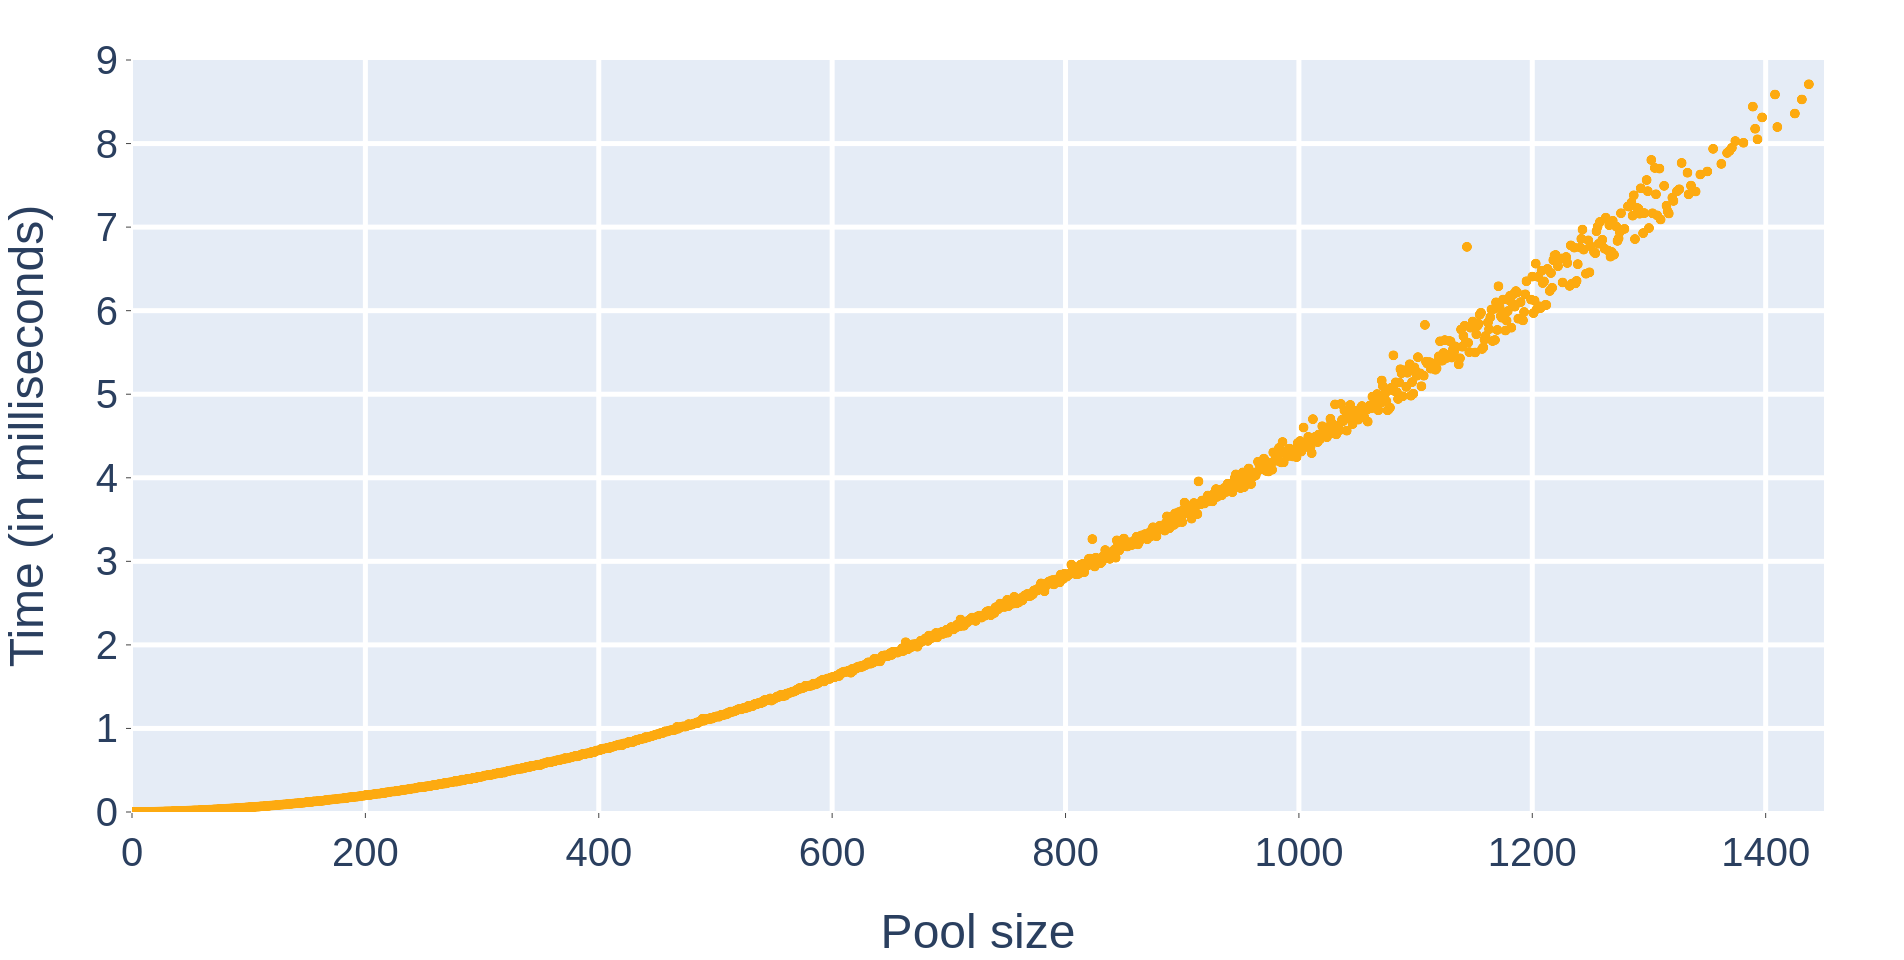
\includegraphics[width=\linewidth]{4 - Sampling/fig/standard/standard_times_all_averages.png}
    \caption{Average infector runtime (in milliseconds) per pool size using \textsc{All-to-All}. Simulation run on 11M population for 100 days without holidays using 1 thread (configurations in Appendix \ref{appendix:configurations}).}
    \label{fig:standard_times_all_averages}
\end{figure}

\begin{figure}
    \centering
    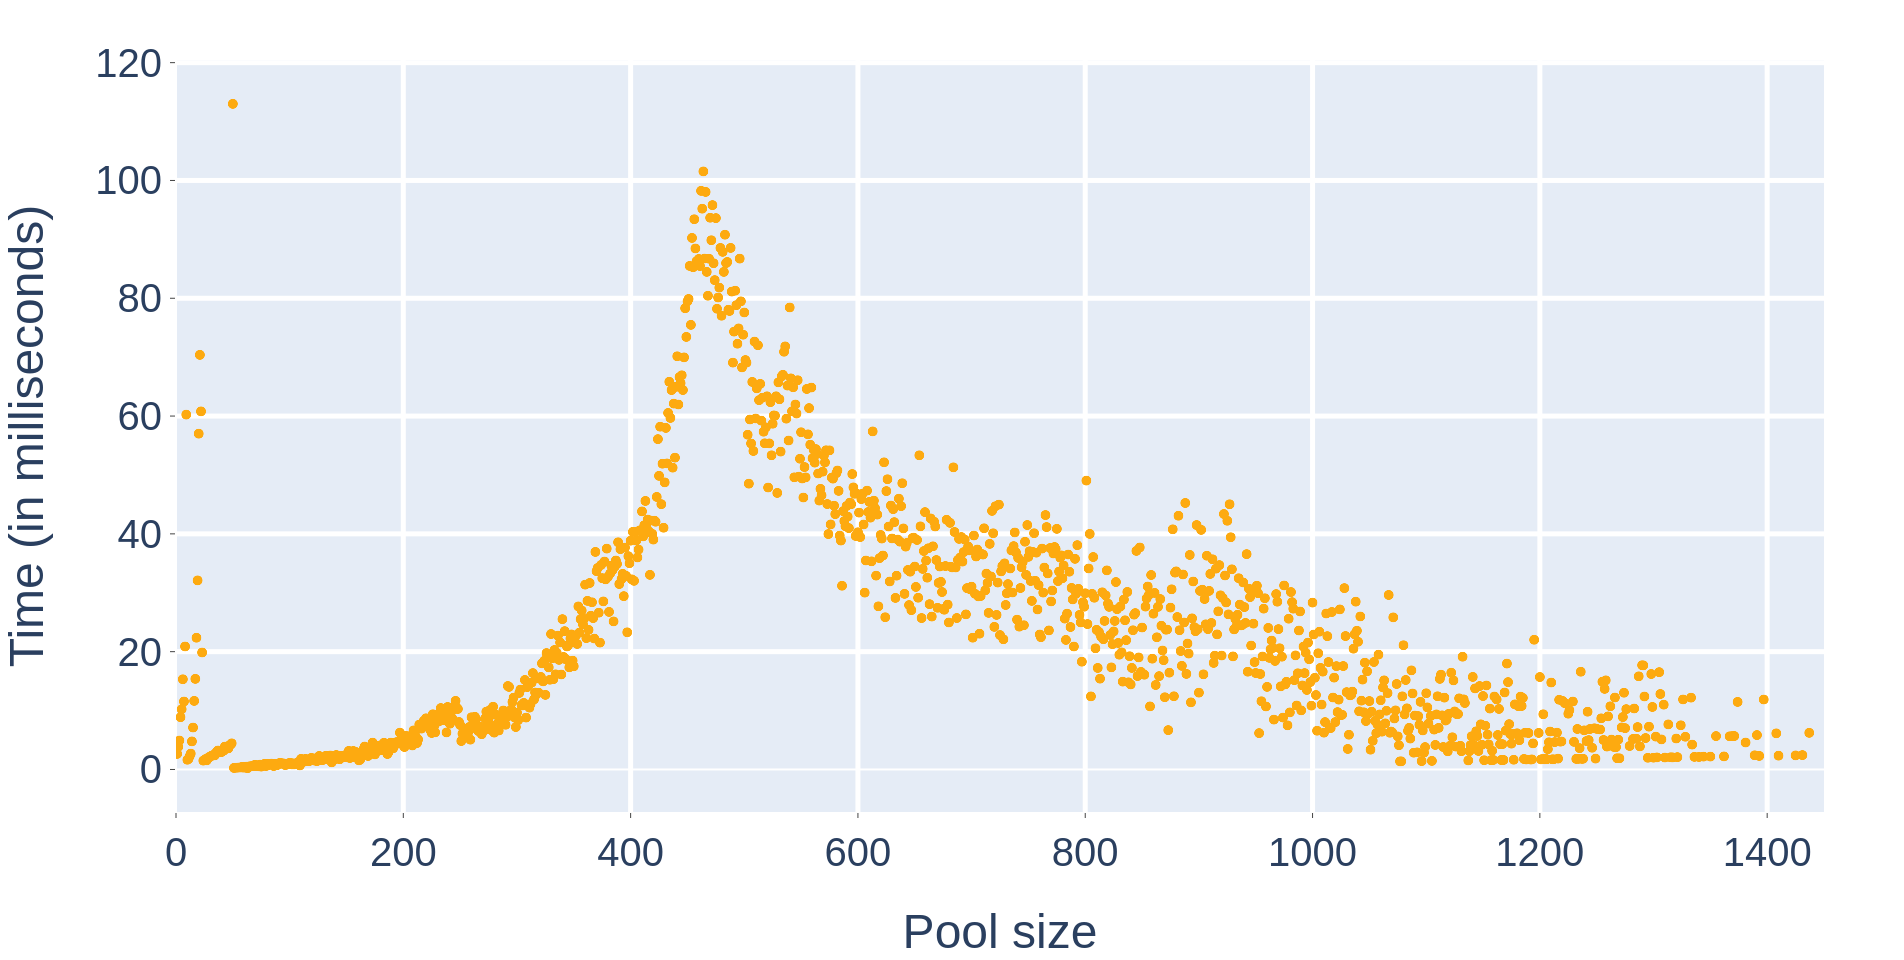
\includegraphics[width=\linewidth]{4 - Sampling/fig/standard/standard_times_all_totals_weekly.png}
    \caption{Total daily average infector runtime (in milliseconds) per pool size using \textsc{All-to-All}, based on a 7-day week. Simulation run on 11M population for 7 days without holidays using 1 thread (configurations in Appendix \ref{appendix:configurations}).}
    \label{fig:standard_times_all_totals_weekly}
\end{figure}

\subsubsection{Pool type runtimes}
Let it be noted that Figures \ref{fig:standard_times_all_averages} and \ref{fig:standard_times_all_totals_weekly} only present the results of measuring the time it takes for the \textsc{All-to-All} algorithm to calculate the contacts and transmissions for a pool with microsecond precision. The graph of Figure \ref{fig:standard_times_all_totals_weekly} reminds us of the pool size distributions of the primary and secondary community contact pools, which were discussed in Section \ref{subsec:contact_pools_data}, but we cannot say this with certainty. In order to get the most complete understanding of the infector runtimes, we also need to know how the different pool types influence the simulation runtime.
\\\\
Figure \ref{fig:standard_times_all_totals_weekly} displayed the total daily average runtimes in function of the pool size, but Figure \ref{fig:standard_times_type_totals} displays these results in function of the pool types and makes a distinction between two different measurements per pool type. \textit{Algorithm only} represents the total time spent in the infector algorithm for all the pools of a pool type. \textit{Total time} gives a more complete overview of the simulation time per pool type, by measuring the time it takes to iterate over all of the pools of a certain type and call infector on them. This distinction needs to be made, because otherwise we could get the wrong impressions of how the time is distributed. For example, all household pools combined only require 0.03 seconds in the algorithm, but it takes our model 1.72 seconds to iterate over every household to calculate their contacts and transmissions. This demonstrates that there is definitely some overhead that we cannot change, which is not surprising since Stride needs to iterate over almost five million households every day.
\\\\
What is most noteworthy about these results, are the proportions between the community pools and the rest. Both of them contain only 22,000 pools, but they account for the vast majority of the total infector runtime. This proves yet again that the larger pools are the main reason the simulation has suboptimal runtimes and that, in theory, our sampling approach will greatly improve this because of its linear time complexity. The difference between the primary and secondary community is due to the way we calculate the impact of every pool, which we previously explained.

\begin{figure}
    \centering
    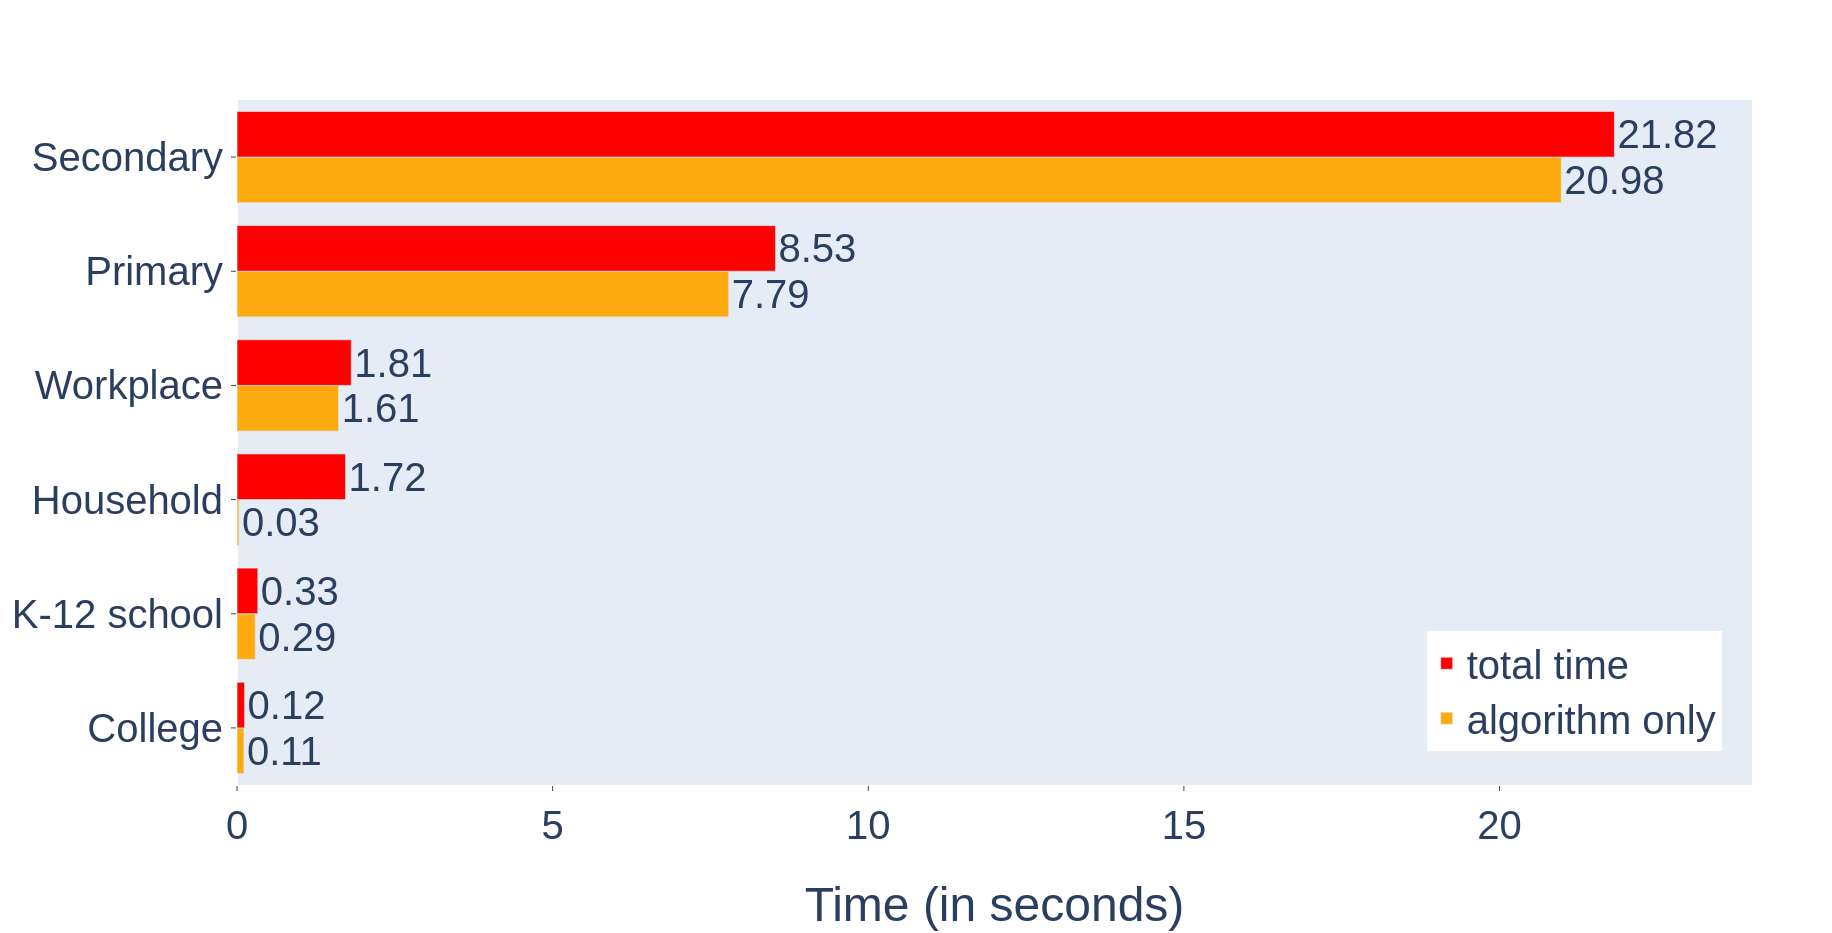
\includegraphics[width=\linewidth]{4 - Sampling/fig/standard/standard_times_type_totals.png}
    \caption{Total daily average infector runtime (in milliseconds) per pool type using \textsc{All-to-All}, based on a 7-day week. \textit{Total time} represents the time it takes to call infector on all of the pools and \textit{algorithm only} represents the total time spent in the infector for a pool type. Simulation run on 11M population for 7 days without holidays using 1 thread (configurations in Appendix \ref{appendix:configurations}).}
    \label{fig:standard_times_type_totals}
\end{figure}

\subsection{Reversed contact vector}
\label{subsec:reversed_contact_vector}
Stride has a built-in unit-testing feature designed to assist the programmers when developing. It tests the program on the basis of different parameters to see if the results, for example the number of infected people, are correct. Because there is randomness involved in a simulation, these results can differ every time. In order to determine whether the results are `correct', they need to lie within certain margins. This tool also verifies that the results are correct when using parallellization, which is necessary to catch multithreading issues such as race conditions \cite{race_condition}. This has proven useful during this thesis, but we will see in the upcoming sections that it does not always succeed in catching erroneous results. Therefore, we introduce another tool that will act as a benchmark in the upcoming sections, which is the reversed contact vector. From Section \ref{subsec:contact_matrix} we know that Stride uses the contact vectors to calculate the contact probabilities that are being used by the infector algorithms. The reversed contact vectors are the reconstructions of those original ones and are built up from the results of a simulation.
\\\\
Figure \ref{fig:reversed_cr_standard} shows the reversed contact vectors of Stride for every pool type and compares them with the original contact vectors. We can clearly see that they are not an exact match, but this is due to the adjustment factors that are taken into account when calculating the contact probabilities, as shown in Algorithm \ref{alg:contact_probability}. The original contact vectors start from the age of one, while Stride starts from age zero, which causes the reversed vectors to shift a little bit to the left. The K-12 school and college contact pools use the school contact vector for their contact probabilities and are therefore both compared to this vector.
\\\\
Figures \ref{fig:reversed_cr_standard_k12school}, \ref{fig:reversed_cr_standard_college} and \ref{fig:reversed_cr_standard_workplace} show that the reversed contact rate for some ages are zero. The reason for this is the way these reversed vectors are built. The results that our tool uses, are generated by an actual Stride simulation. They are saved in a file that contains all the logged events among which the contacts, transmissions, etc. These events are saved line by line and specify the IDs of both individuals in an event, their ages, the probability that the event would happen, and many more. If every single event in a simulation would be logged, the size of the log file would be several gigabytes per day for the 600K population. To determine how much needs to be logged, a parameter can be set for the number of people that need to be tracked. These people are then randomly chosen when initialising the simulator and only their events are logged. Our reversed contact rates also do not take into account that someone might not be a member of a certain pool type, such as an unemployed adult or an adult that works but who is not a teacher and thus has zero contacts at a school. This is the reason that the reversed rates for some ages are noticeably less than the original ones.
\\\\
In order to get the best results for these reversed contact vectors, we set the number of infected people in the beginning to zero. This leads to no infections during the entire simulation so individuals would not change their behaviour because they are infected. We set the number of people that will be logged to 50,000 and only simulate 28 days for these results, which is enough to get accurate results for every pool type. A side effect of this method is that some ages for which there are not that many individuals in a particular pool type, the results may show that the contact rate is zero. This is due to the random selection of people that need to be tracked, which causes some ages to not be represented in a pool type. An example of this are the professors of a college, ages 23 to 65, for which Figure \ref{fig:reversed_cr_standard_college} shows they do not have any contacts which is not true. The other possibility for this to happen is that there are no individuals in the population that meet the criteria for a certain age and pool type. All in all the reversed contact vectors still provide enough data to evaluate the model. In the upcoming sections we will ignore the original contact rates and only use the reversed vectors from Figure \ref{fig:reversed_cr_standard} as reference point.

\begin{figure}
    \centering
    \begin{subfigure}{.8\linewidth}
        \centering
        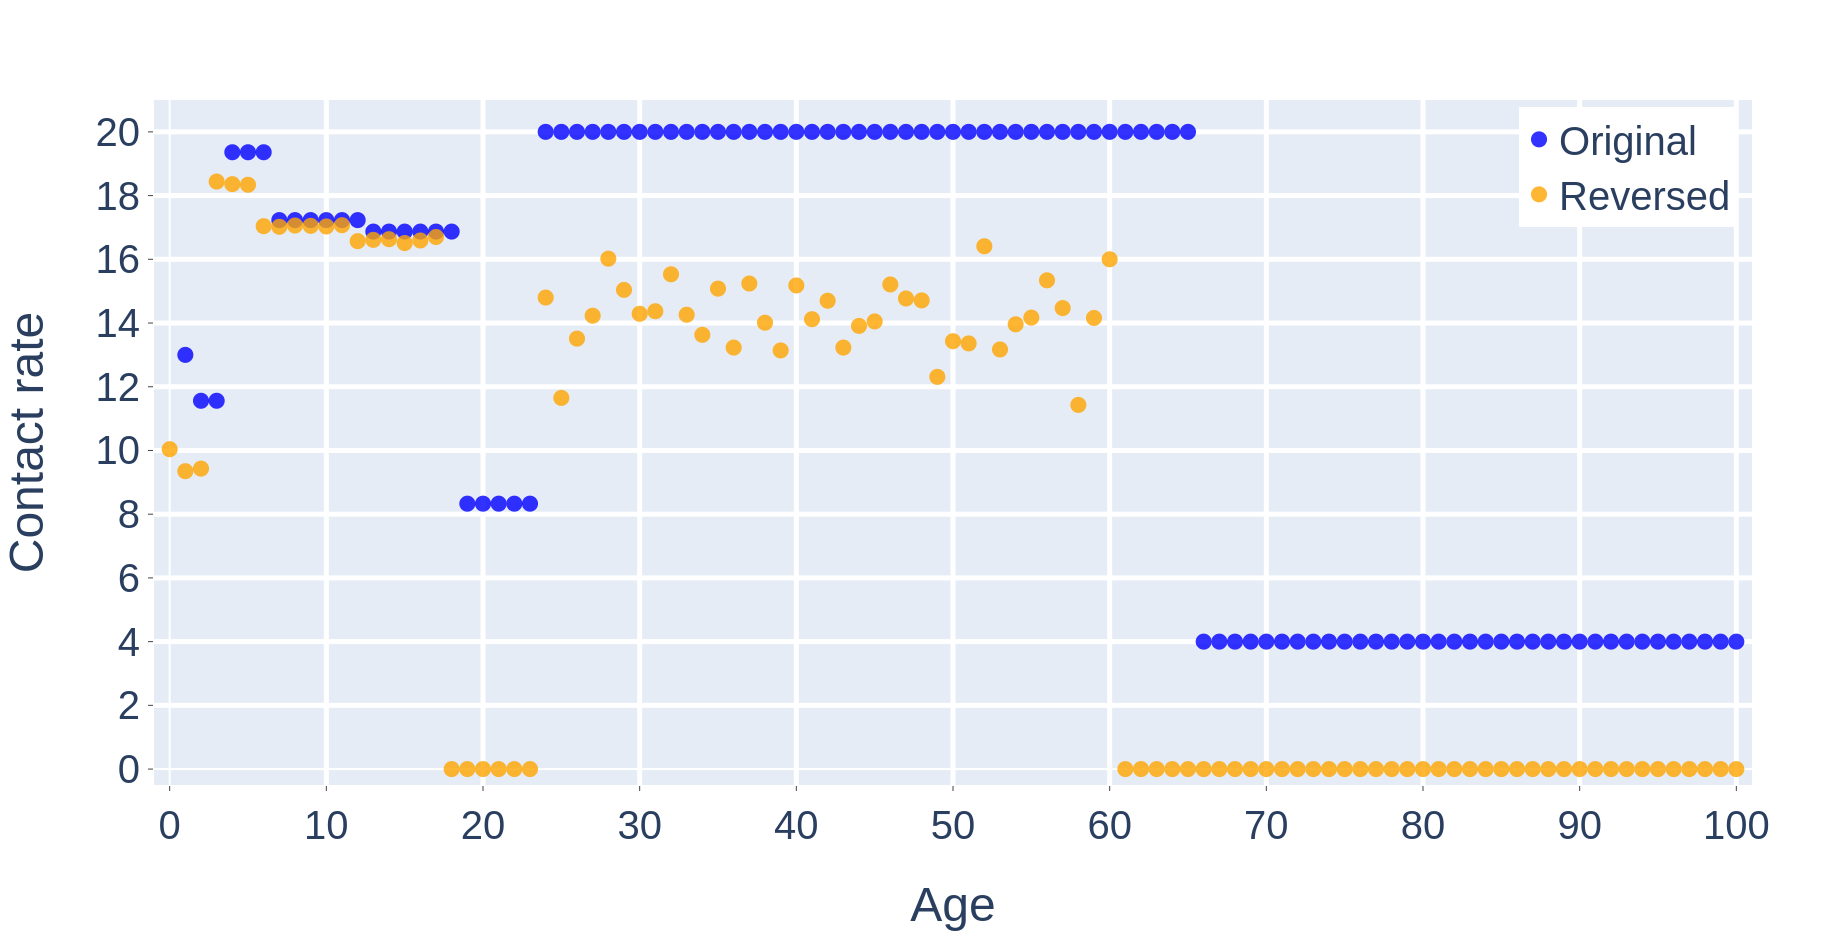
\includegraphics[width=\textwidth]{4 - Sampling/fig/standard/standard_reverse_cr_k12school.png}
        \caption{K-12 school}
        \label{fig:reversed_cr_standard_k12school}
    \end{subfigure}
    \begin{subfigure}{.8\linewidth}
        \centering
        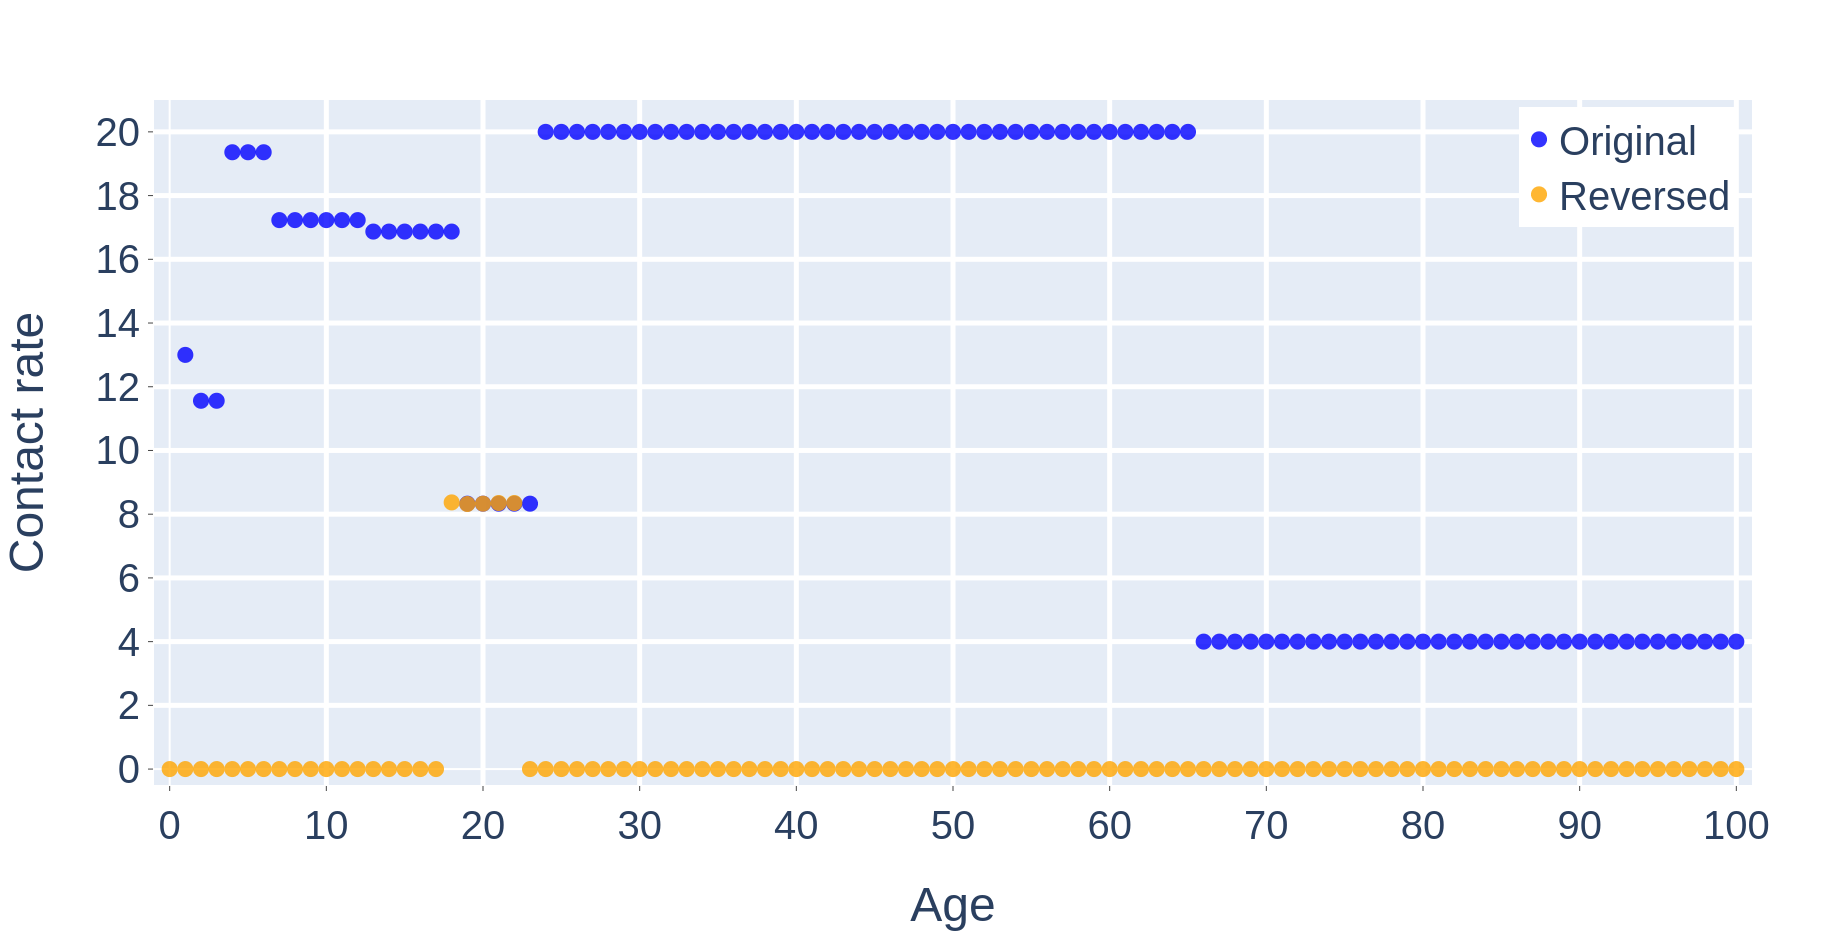
\includegraphics[width=\textwidth]{4 - Sampling/fig/standard/standard_reverse_cr_college.png}
        \caption{College}
        \label{fig:reversed_cr_standard_college}
    \end{subfigure}
    \begin{subfigure}{.8\linewidth}
        \centering
        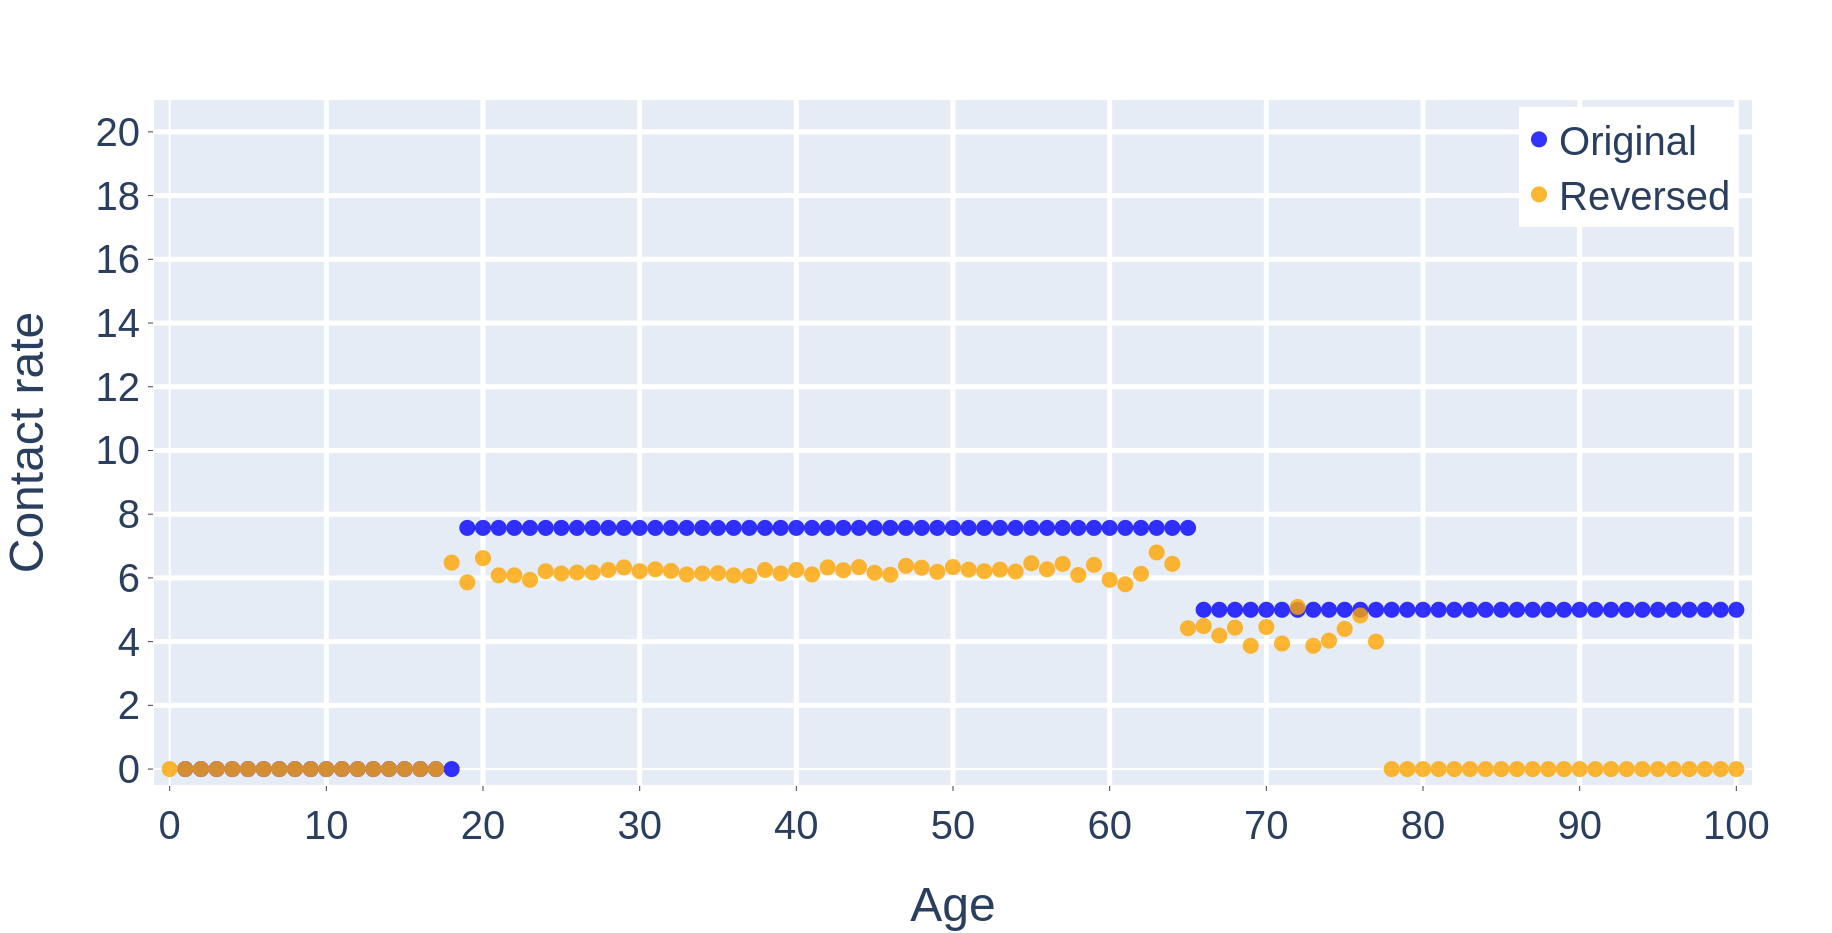
\includegraphics[width=\textwidth]{4 - Sampling/fig/standard/standard_reverse_cr_workplace.png}
        \caption{Workplace}
        \label{fig:reversed_cr_standard_workplace}
    \end{subfigure}
    \caption{Comparison of the reversed contact rates with the original contact rates from Section \ref{subsec:contact_matrix}.}
\end{figure}
\begin{figure}\ContinuedFloat
    \centering
    \begin{subfigure}{.8\linewidth}
        \centering
        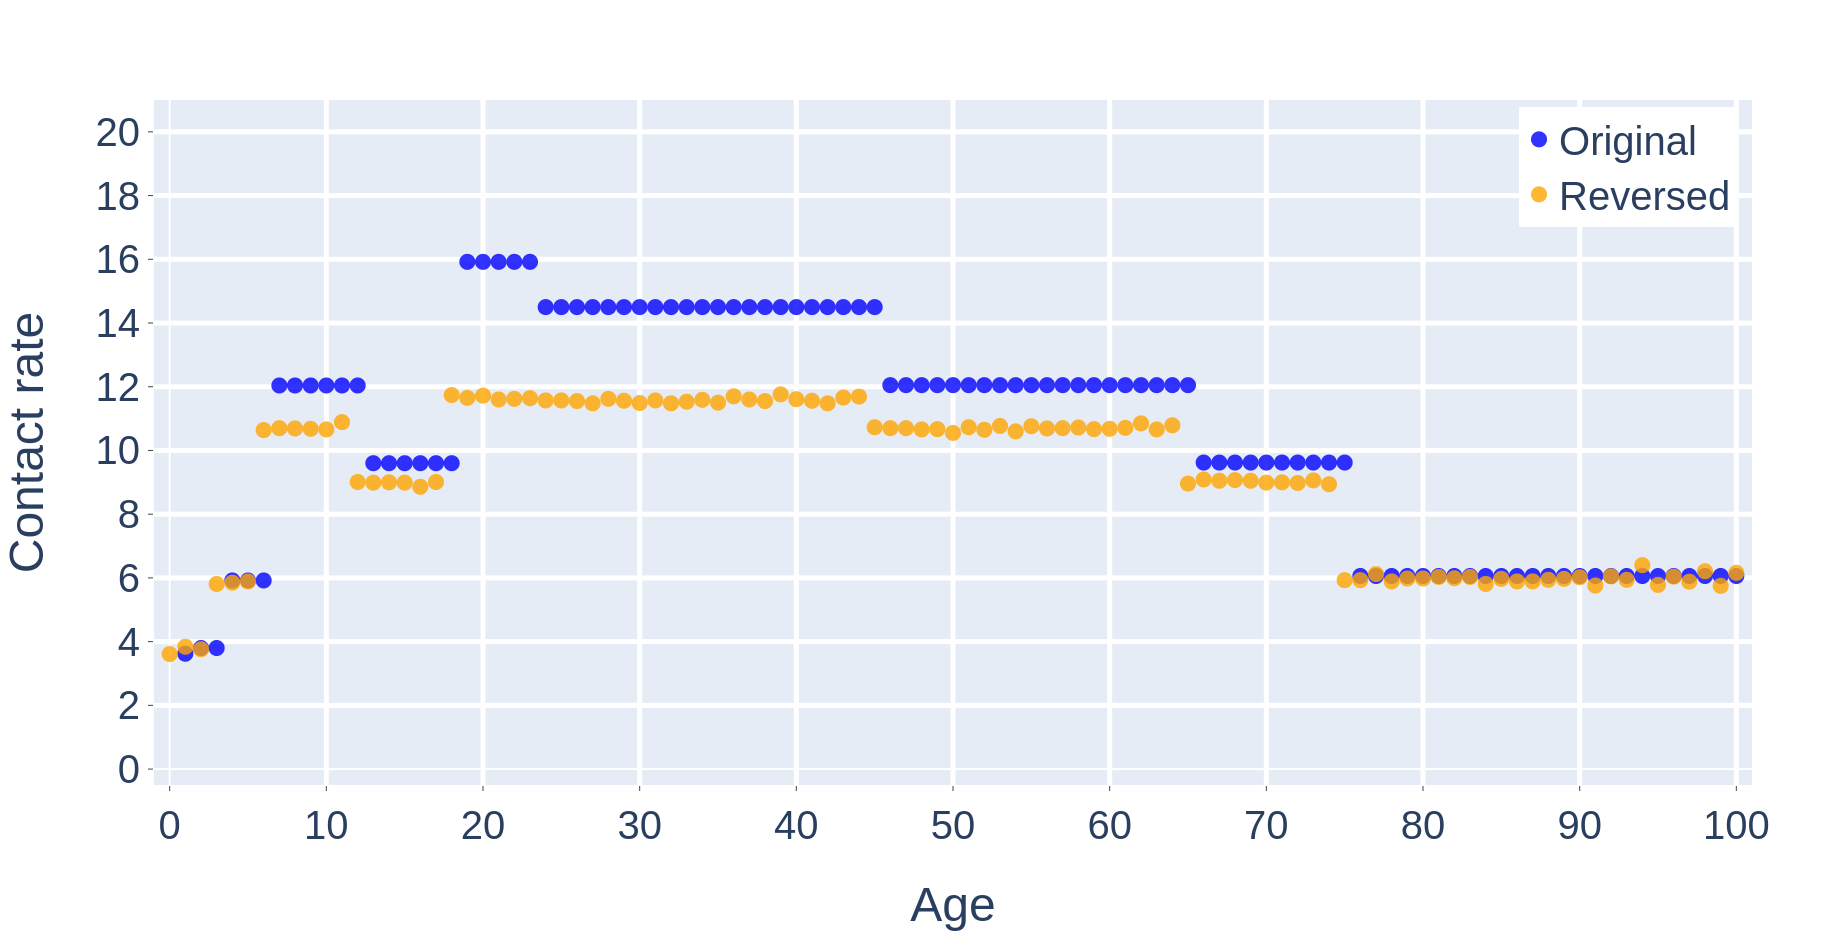
\includegraphics[width=\textwidth]{4 - Sampling/fig/standard/standard_reverse_cr_primary.png}
        \caption{Primary community}
        \label{fig:reversed_cr_standard_primary}
    \end{subfigure}
    \begin{subfigure}{.8\linewidth}
        \centering
        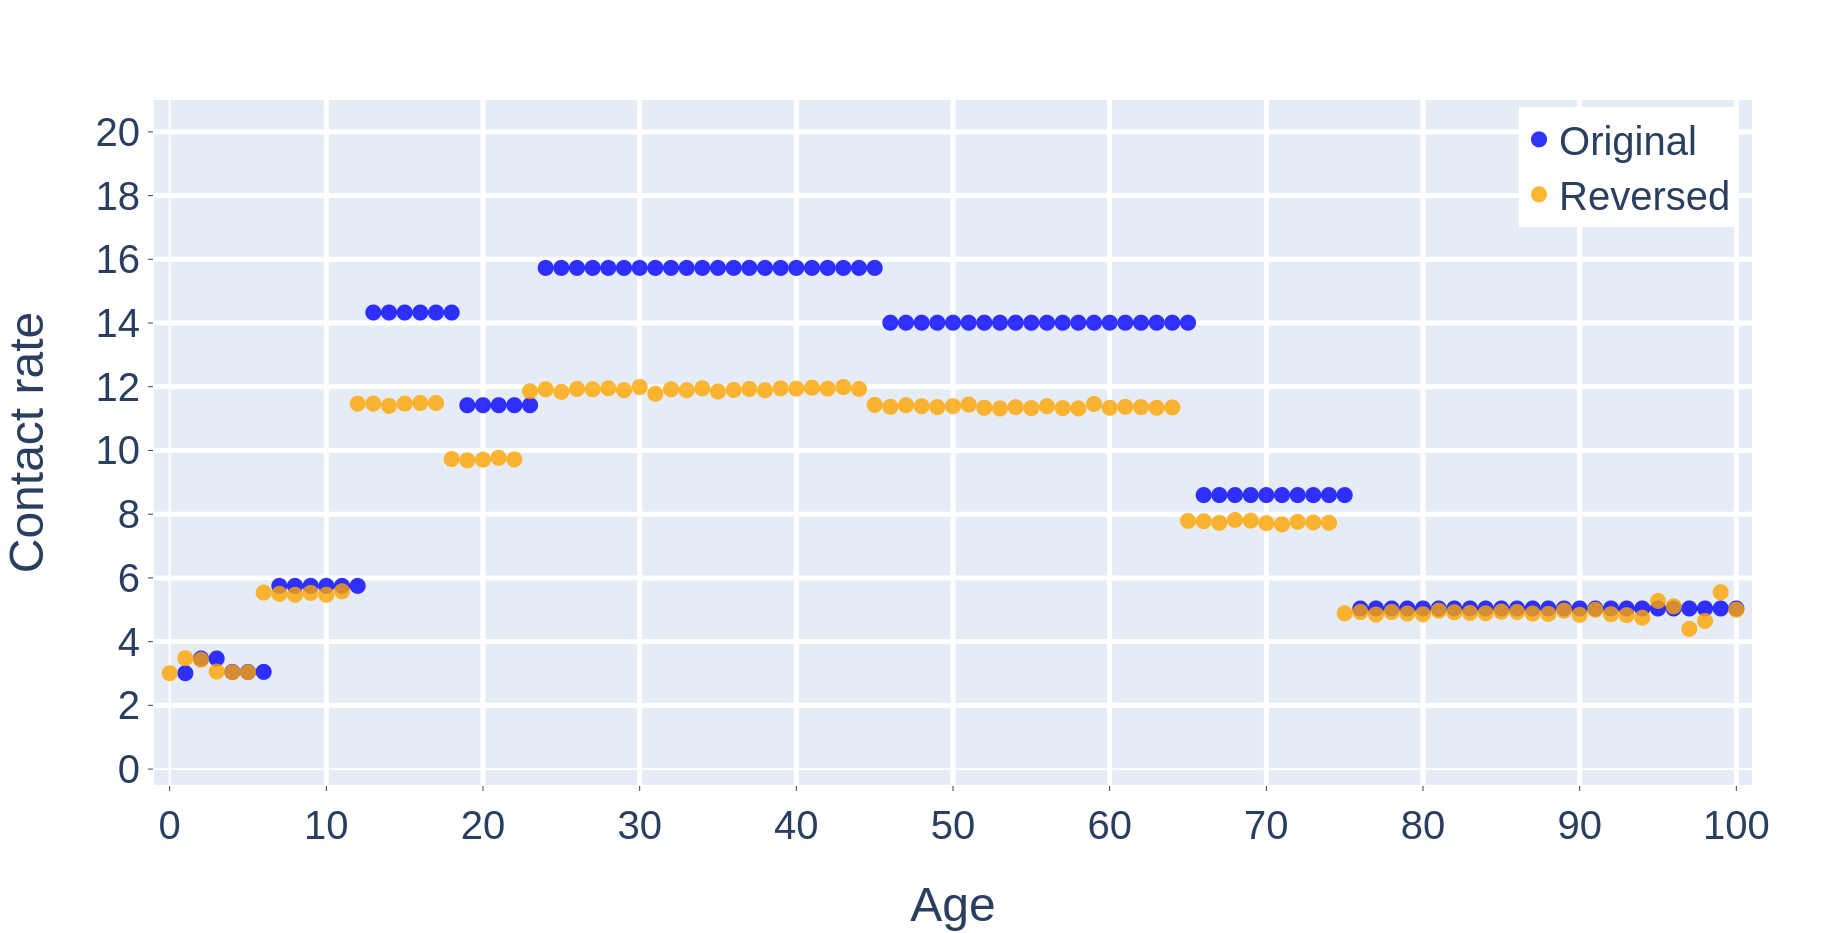
\includegraphics[width=\textwidth]{4 - Sampling/fig/standard/standard_reverse_cr_secondary.png}
        \caption{Secondary community}
        \label{fig:reversed_cr_standard_secondary}
    \end{subfigure}
    \caption{Comparison of the reversed contact rates with the original contact rates from Section \ref{subsec:contact_matrix}.}
    \label{fig:reversed_cr_standard}
\end{figure}

\section{Iterative intervals}
\label{sec:iterative_intervals}
Our general idea is to use a sampling approach to optimise the \textsc{All-to-All} infector algorithm. However, as we discussed, the main issue for this is the contact probability between two individuals, which is calculated based on the age of the two individuals. In order to use our approach, this issue first must be resolved. This section explains a solution for the contact probability calculations, which also happens to be a major improvement already.

\subsection{Age intervals}
\label{subsec:age_intervals}
Since our problem is about the calculation of the contact probabilities, this is where we should look for the solution. Algorithm \ref{alg:contact_probability} shows how this calculation uses the contact rates of two persons and takes the minimum of the two rates to determine the probability. If we want to take a sample from a pool with the binomial distribution we talked about, we would need a contact probability that applies to everyone in the pool. Unfortunately, this is not possible because the contact rates are different depending on age. However, if we look at the contact vectors in Section \ref{subsec:contact_matrix}, we notice that the contact rates are the same for a lot of ages. This means that the contact probability in one pool is the same in a lot of cases. Thus, we could use the same contact probability for different pairs of individuals and still get correct results. Following this logic, we split up the contact pools in groups, where everyone in a group has the same contact rate. Then, if our model were to calculate the contacts for a pool, it would only need to calculate one contact probability for every pair of groups. Although the infector would still have a quadratic time complexity since everyone still gets compared with everyone, it would reduce the runtime by reducing the number of contact probabilities that need to be calculated.
\\\\
We now need to determine for every pool type how the pool members will be divided in groups. For this we look at the contact vectors from Section \ref{subsec:contact_matrix} to decide the ages with the same contact rate. Because the ages with the same contact rate lie in age intervals for every pool type, we can simply use these age intervals to represent a `same contact rate group'. Table \ref{tab:age_intervals} shows the age intervals for every contact pool type with their corresponding contact rates. The first age intervals for the primary and secondary community have two contact rates, because age one has a different rate (the upper one) than ages two and three. Since these rates are almost the same, we choose to not split them up. However, for the school contact type we have a separate interval for age one, because its rate is much more different. Another reason for splitting these up or not, is the way these ages are distributed in the pools. In a school contact pool, almost everyone except the teacher has the same age, while a community pool can contain all the possible ages. This results in less intervals for the community pools, which will be beneficial for our sampling approach in the next sections. When we now determine the contact probability between two intervals, we use the age of the first member of an interval. Intervals that contain ages with multiple contact rates will thus be represented by the contact rate of the first member, which can be different depending on the pool since people in a pool do not have a predetermined order.

\begin{table}
    \centering
    \begin{subtable}[b]{0.45\textwidth}
        \centering
        \begin{tabular}{@{}ccr@{}}
            \toprule
            \# & Age interval & Rate \\ \midrule
            1 & {[} 1 {]} & 13.00 \\
            2 & {[} 2, 3 {]} & 11.56 \\
            3 & {[} 4, 6 {]} & 19.36 \\
            4 & {[} 7, 12 {]} & 17.23 \\
            5 & {[} 13, 18 {]} & 16.87 \\
            6 & {[} 19, 23 {]} & 8.33 \\
            7 & {[} 24, 65 {]} & 20.00 \\
            8 & {[} 66, $\infty$ {[} & 4 \\ \bottomrule
        \end{tabular}
        \caption{School (K-12 school and college).}
        \label{tab:age_intervals_school}
    \end{subtable}
    \hfill
    \begin{subtable}[b]{0.45\textwidth}
        \centering
        \begin{tabular}{ccr}
            \hline
            \# & \multicolumn{1}{l}{Age interval} & \multicolumn{1}{l}{Rate} \\ \hline
            1 & {[} 0, 18 {]} & 0 \\
            2 & {[} 19, 65 {]} & 7.57 \\
            3 & {[} 66, $\infty$ {[} & 5.00 \\ \hline
        \end{tabular}
        \caption{Workplace}
        \label{tab:age_intervals_workplace}
    \end{subtable}
    \newline
    \newline
    \begin{subtable}[h]{0.45\textwidth}
        \centering
        \begin{tabular}{ccr}
            \hline
            \# & \multicolumn{1}{l}{Age interval} & Rate \\ \hline
            1 & {[} 0, 3 {]} & \begin{tabular}[c]{@{}r@{}}3.62\\ 3.80\end{tabular} \\
            2 & {[} 4, 6 {]} & 5.92 \\
            3 & {[} 7, 12 {]} & 12.04 \\
            4 & {[} 13, 18 {]} & 9.60 \\
            5 & {[} 19, 23 {]} & 15.92 \\
            6 & {[} 24, 45 {]} & 14.50 \\
            7 & {[} 46, 65 {]} & 12.05 \\
            8 & {[} 66, 75 {]} & 9.62 \\
            9 & {[} 75, $\infty$ {[} & 6.06 \\ \hline
        \end{tabular}
        \caption{Primary community.}
        \label{tab:age_intervals_primary}
    \end{subtable}
    \hfill
    \begin{subtable}[h]{0.45\textwidth}
        \centering
        \begin{tabular}{ccr}
            \hline
            \# & \multicolumn{1}{l}{Age interval} & Rate \\ \hline
            1 & {[} 0, 3 {]} & \begin{tabular}[c]{@{}r@{}}3.01\\ 3.47\end{tabular} \\
            2 & {[} 4, 6 {]} & 3.05 \\
            3 & {[} 7, 12 {]} & 5.75 \\
            4 & {[} 13, 18 {]} & 14.33 \\
            5 & {[} 19, 23 {]} & 11.42 \\
            6 & {[} 24, 45 {]} & 15.73 \\
            7 & {[} 46, 65 {]} & 14.01 \\
            8 & {[} 66, 75 {]} & 8.60 \\
            9 & {[} 75, $\infty$ {[} & 5.04 \\ \hline
        \end{tabular}
        \caption{Secondary community.}
        \label{tab:age_intervals_secondary}
    \end{subtable}
    \caption{Age intervals for the different contact pool types with their corresponding contact rates. The intervals with multiple contact rates are represented by the rate of the first member, which is random and thus different per pool.}
    \label{tab:age_intervals}
\end{table}

\subsection{Implementation}
\label{subsec:implementation_iterative_intervals}
Now we can use the age intervals to implement our improved algorithm. Algorithm \ref{alg:age_sorting} presents the pseudo code for the sorting of pool members in these different intervals, which also returns the number of members in every interval. This sorting function will also be used for the upcoming approaches in the next sections. The implementation of our approach that uses the age intervals is presented in Algorithm \ref{alg:iterative_intervals}. The household pools still use the original \textsc{All-to-All} algorithm, since they contain maximum six persons. The rest of the pools use our intervals approach, where every intervals gets compared with every other interval including itself. For every pair of intervals, only one contact probability is calculated. Then, the algorithm iterates over both intervals and uses the contact probability for every pair of members from two intervals to see if they have contact and transmit the disease. Because this algorithm still compares everyone with everyone in a pool by iterating over the intervals and their members, we will refer to this \textsc{All-to-All} infector approach as \textsc{Iterative-intervals} from now on.

\begin{algorithm}
\caption{Pseudo code of the function that sorts the members in age intervals.}
\label{alg:age_sorting}
\begin{algorithmic}[1]
    \Require{$P_{1} \dots P_{N}$, $type$} \Comment{All members of the pool and type of pool}\;
    \Ensure{$P[\;] sorted$, $S[\;]$} \Comment{Sorted members and interval sizes}
    \Statex
    \State $intervals[\;] \gets$ \Call{age\_intervals}{$type$}\Comment{Maximum ages per interval (ascending)}
    \State $N_{intervals} \gets$ \Call{sizeof}{$intervals[\;]$} \Comment{Number of intervals}
    \State $i_{unsorted} \gets 1$\Comment{Index of first unsorted member}
    \State $S[\;] \gets [N_{intervals}]$\Comment{Interval sizes, zero at start}
    \Statex
    \For{$i_{interval} \gets 1$ to ($N_{intervals}-1)$}\Comment{Iterate over the intervals}
        \State $age_{interval} \gets intervals[i_{interval}]$ \Comment{Maximum age of the interval}
        \For{$i_{member} \gets i_{unsorted}$ to $N$}\Comment{Iterate over the unsorted members}
            \State $age_{member} \gets$ \Call{age}{$P[i_{member}]$}
            \If{$age_{member} \leq age_{interval}$}
                \If{$i_{member} > i_{unsorted}$}
                    \State \Call{swap}{$P[i_{unsorted}], P[i_{member}]$}
                \EndIf
                \State $i_{unsorted}++$
                \State $S[i_{interval}]++$
            \EndIf
        \EndFor
    \EndFor
    \State $S[N_{intervals}] \gets N - i_{unsorted} + 1$ \Comment{Remaining unsorted members}
    \Statex
    \State \Return $S[\;]$
\end{algorithmic}
\end{algorithm}

\begin{algorithm}
\caption{Pseudo code of the \textsc{Iterative-intervals} infector.}
\label{alg:iterative_intervals}
\begin{algorithmic}[1]
    \Require{$P_{1} \dots P_{N}$, $type$} \Comment{All members of the pool and type of pool}\;
    \Statex
    \If{$type = household$}
        \State original \textsc{All-to-All} \Comment{Algorithm \ref{alg:all-to-all}}
    \Else
        \State $S[\;] \gets$ \Call{sort\_intervals}{$P[\;], type$}\Comment{Algorithm \ref{alg:age_sorting}}
        \State $N_{intervals} \gets$ \Call{sizeof}{$S[\;]$} \Comment{Number of intervals}
        \Statex
        \For{$interval_{1} \gets 1$ to $N_{intervals}$} \Comment{Iterate intervals}
            \For{$interval_{2} \gets interval_{1}$ to $N_{intervals}$} \Comment{Iterate remaining intervals}
                \State $C_{prob} \gets$ \Call{ContactProbability}{$P[interval_{1}], P[interval_{2}]$}\Comment{Algorithm \ref{alg:contact_probability}}
                \Statex
                \If{$interval_{1}$ = $interval_{2}$}
                    \For{$i \gets 1$ to $S[interval_{1}]$}
                        \State $P_{1} \gets$ member $i$ of $interval_{1}$
                        \If{$P_{1}$ not in pool}
                            \State continue to next $P_{1}$
                        \EndIf
                        \For{$j \gets i$ to $S[interval_{1}]$}
                            \State $P_{2} \gets$ member $j$ of $interval_{1}$
                            \If{$P_{1} = P_{2}$ OR $P_{2}$ not in pool}
                                \State Continue to next $j$
                            \EndIf
                            \If{\Call{BernoulliTrial}{$C_{prob}$}}
                                \State register contact
                                \If{$P_{1}$ or $P_{2}$ susceptible and other infectious}
                                    \State $T_{prob} \gets$ transmission probability
                                    \If{\Call{BernoulliTrial}{$T_{prob}$}}
                                        \State infect the susceptible one
                                    \EndIf
                                \EndIf
                            \EndIf
                        \EndFor
                    \EndFor
                \Else
                    \Foreach{member $P_{1}$ in $interval_{1}$}
                        \If{$P_{1}$ not in pool}
                            \State continue to next $P_{1}$
                        \EndIf
                        \Foreach{member $P_{2}$ in $interval_{2}$}
                            \If{$P_{2}$ not in pool OR $P_{1} = P_{2}$}
                                \State continue to next $P_{2}$
                            \EndIf
                            \If{\Call{BernoulliTrial}{$C_{prob}$}}
                                \State register contact
                                \If{$P_{1}$ or $P_{2}$ susceptible and other infectious}
                                    \State $T_{prob} \gets$ transmission probability
                                    \If{\Call{BernoulliTrial}{$T_{prob}$}}
                                        \State infect the susceptible one
                                    \EndIf
                                \EndIf
                            \EndIf
                        \EndForeach
                    \EndForeach
                \EndIf
            \EndFor
        \EndFor
    \EndIf
\end{algorithmic}
\end{algorithm}

\subsection{Correctness}
\label{subsec:correctness_iterative_intervals}
We need to evaluate our approach and see if our model logic has not changed. For this we use the techniques discussed in Section \ref{subsec:reversed_contact_vector}, which are the built-in testing tool and the reversed contact vector. The testing tool only tells us if the range of the results are valid, which is the case. We then continue to compute the reversed contact rates, for which the results are displayed in Figure \ref{fig:ii_vs_standard_reverse_cr}. They show that the \textsc{Iterative-intervals} approach has almost identical reversed contact rates as the original \textsc{All-to-All} algorithm. Therefore, we conclude that \textsc{Iterative-intervals} is a valid \textsc{All-to-All} algorithm.

\begin{figure}
    \centering
    \begin{subfigure}{.8\linewidth}
        \centering
        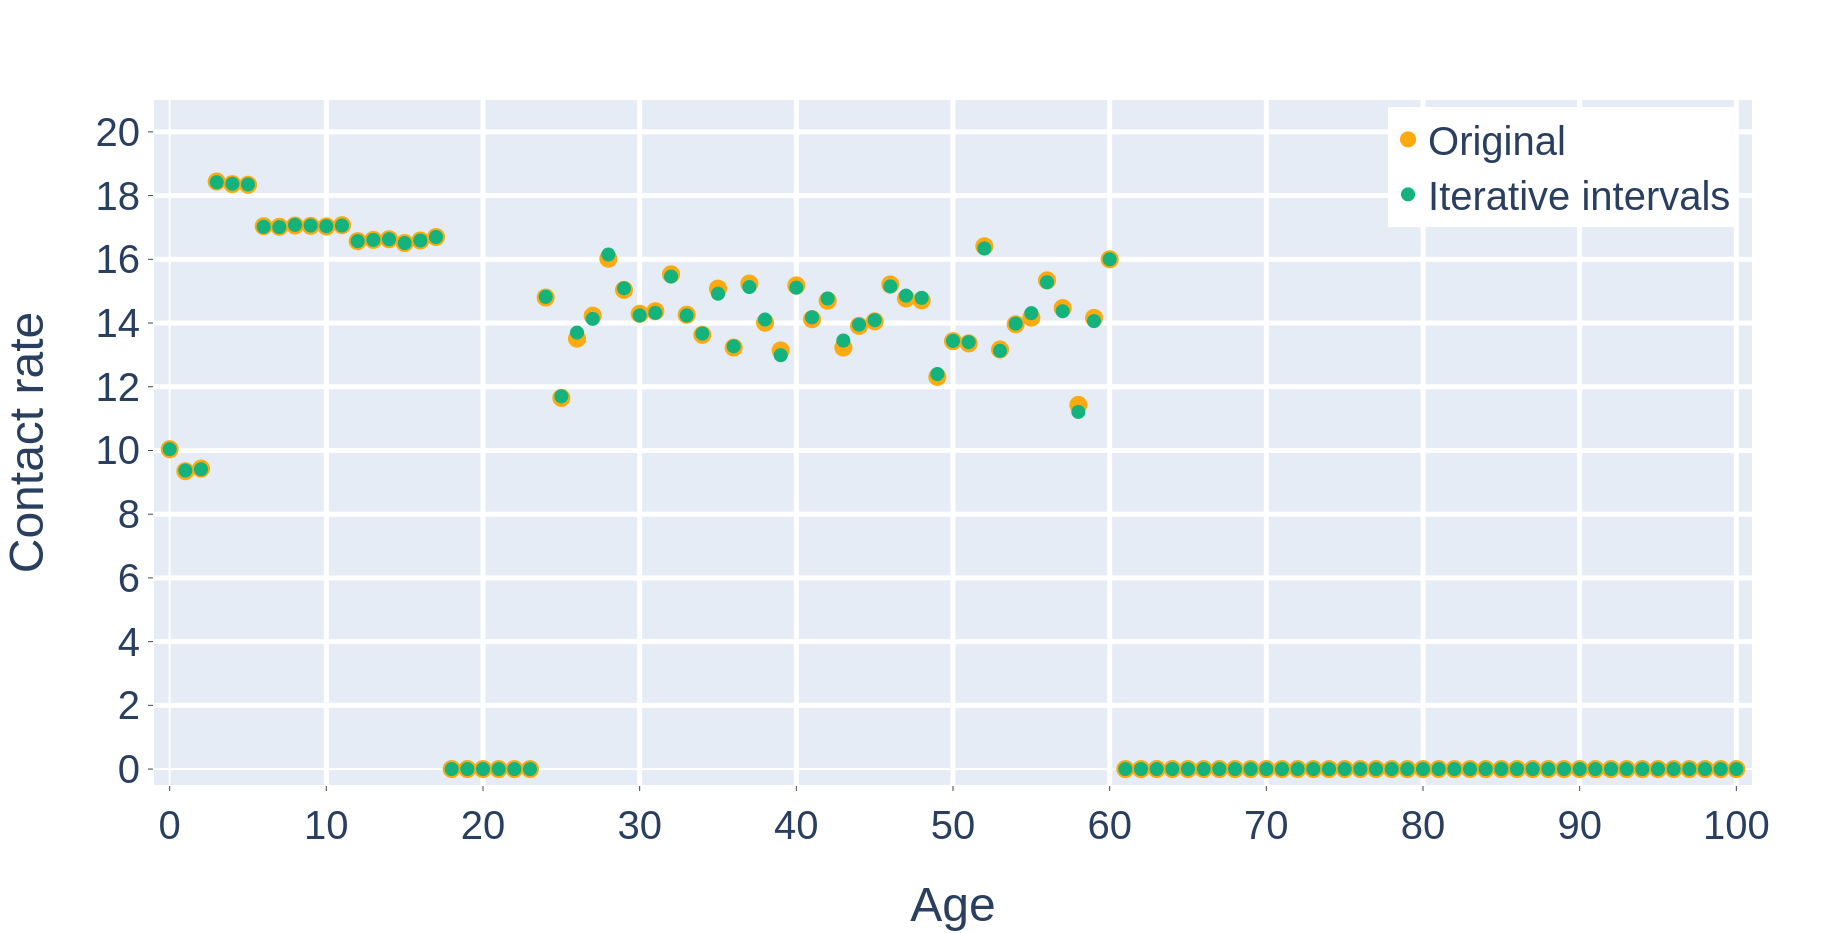
\includegraphics[width=\textwidth]{4 - Sampling/fig/iterative_intervals/ii_vs_standard_reverse_cr_k12school.png}
        \caption{K-12 school}
        \label{fig:ii_vs_standard_reversed_cr_standard_k12school}
    \end{subfigure}
    \begin{subfigure}{.8\linewidth}
        \centering
        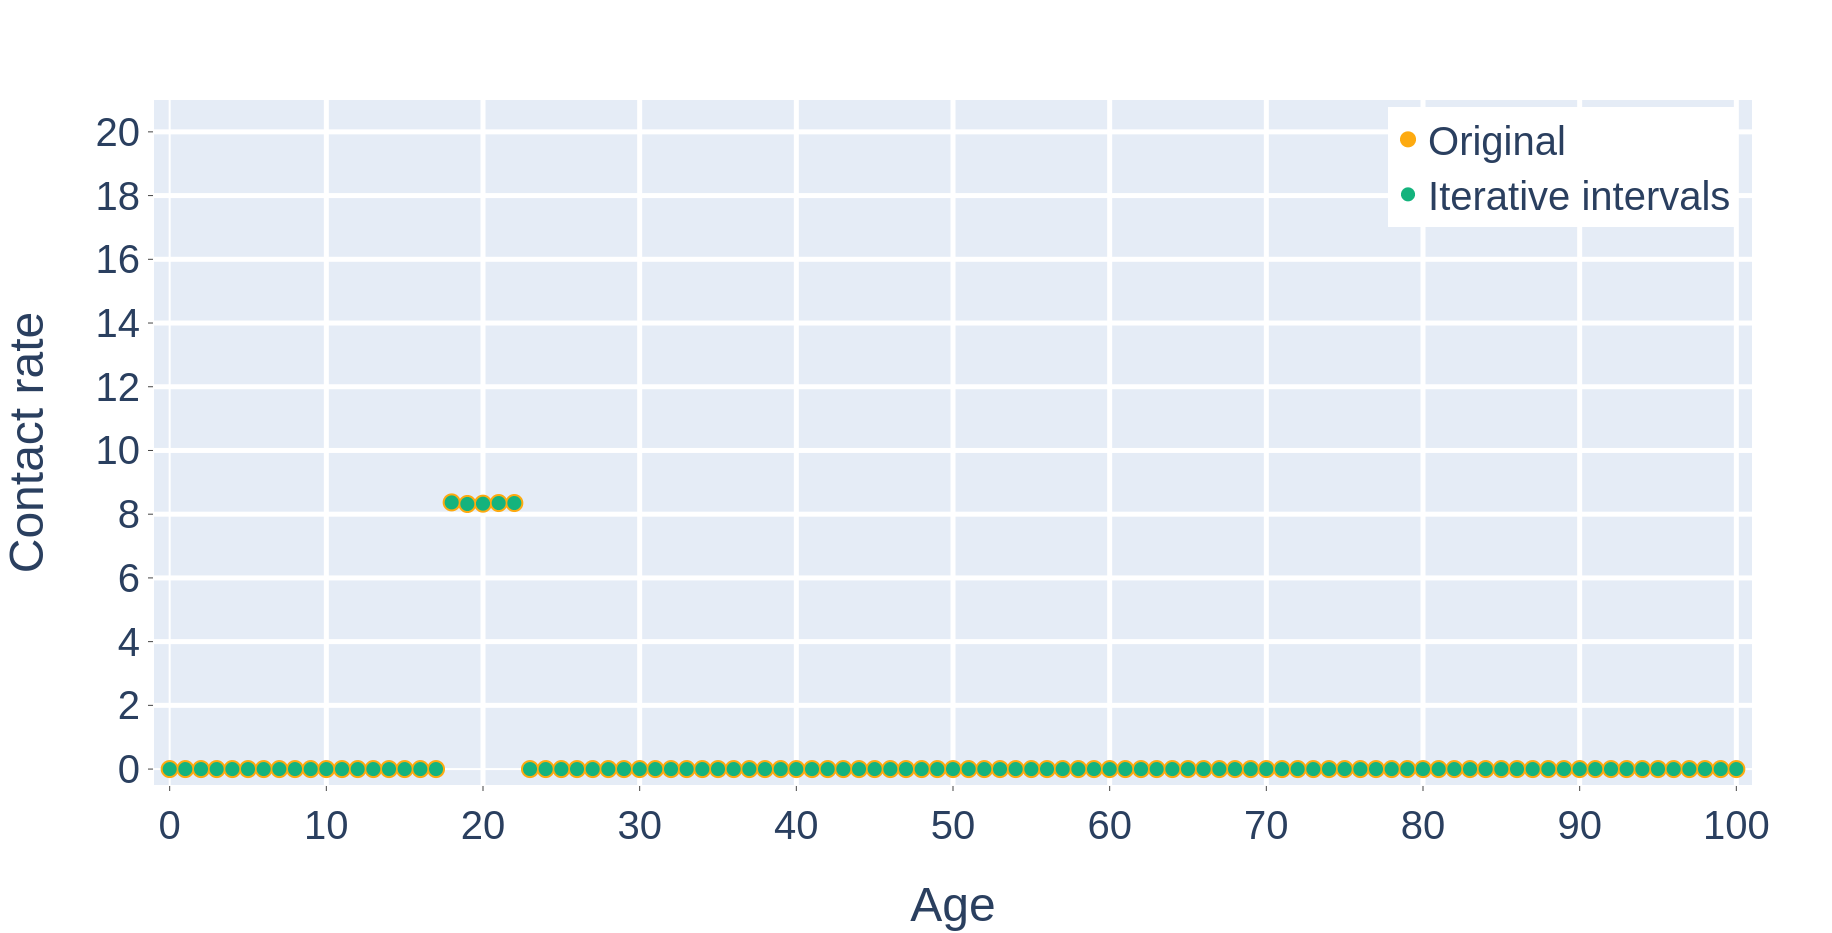
\includegraphics[width=\textwidth]{4 - Sampling/fig/iterative_intervals/ii_vs_standard_reverse_cr_college.png}
        \caption{College}
        \label{fig:ii_vs_standard_reversed_cr_standard_college}
    \end{subfigure}
    \begin{subfigure}{.8\linewidth}
        \centering
        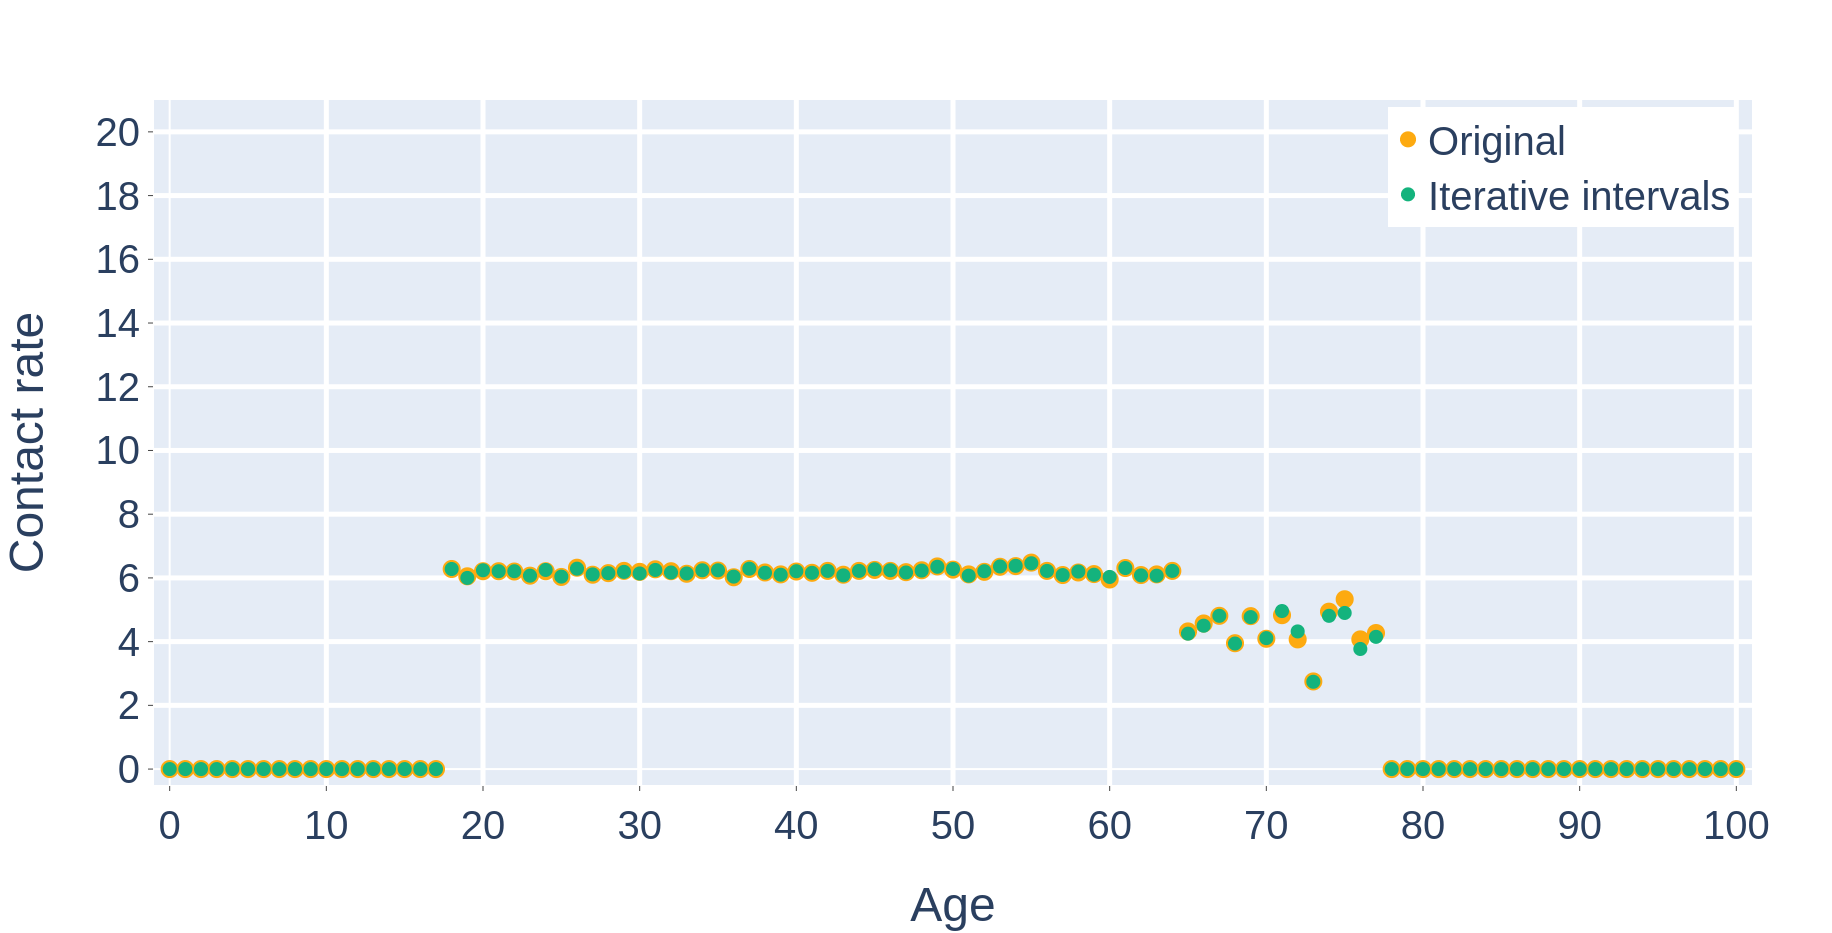
\includegraphics[width=\textwidth]{4 - Sampling/fig/iterative_intervals/ii_vs_standard_reverse_cr_workplace.png}
        \caption{Workplace}
        \label{fig:ii_vs_standard_reversed_cr_standard_workplace}
    \end{subfigure}
    \caption{Comparison of the \textsc{Iterative-intervals} reversed contact rates with the original \textsc{All-to-All} reversed contact rates.}
\end{figure}
\begin{figure}\ContinuedFloat
    \centering
    \begin{subfigure}{.8\linewidth}
        \centering
        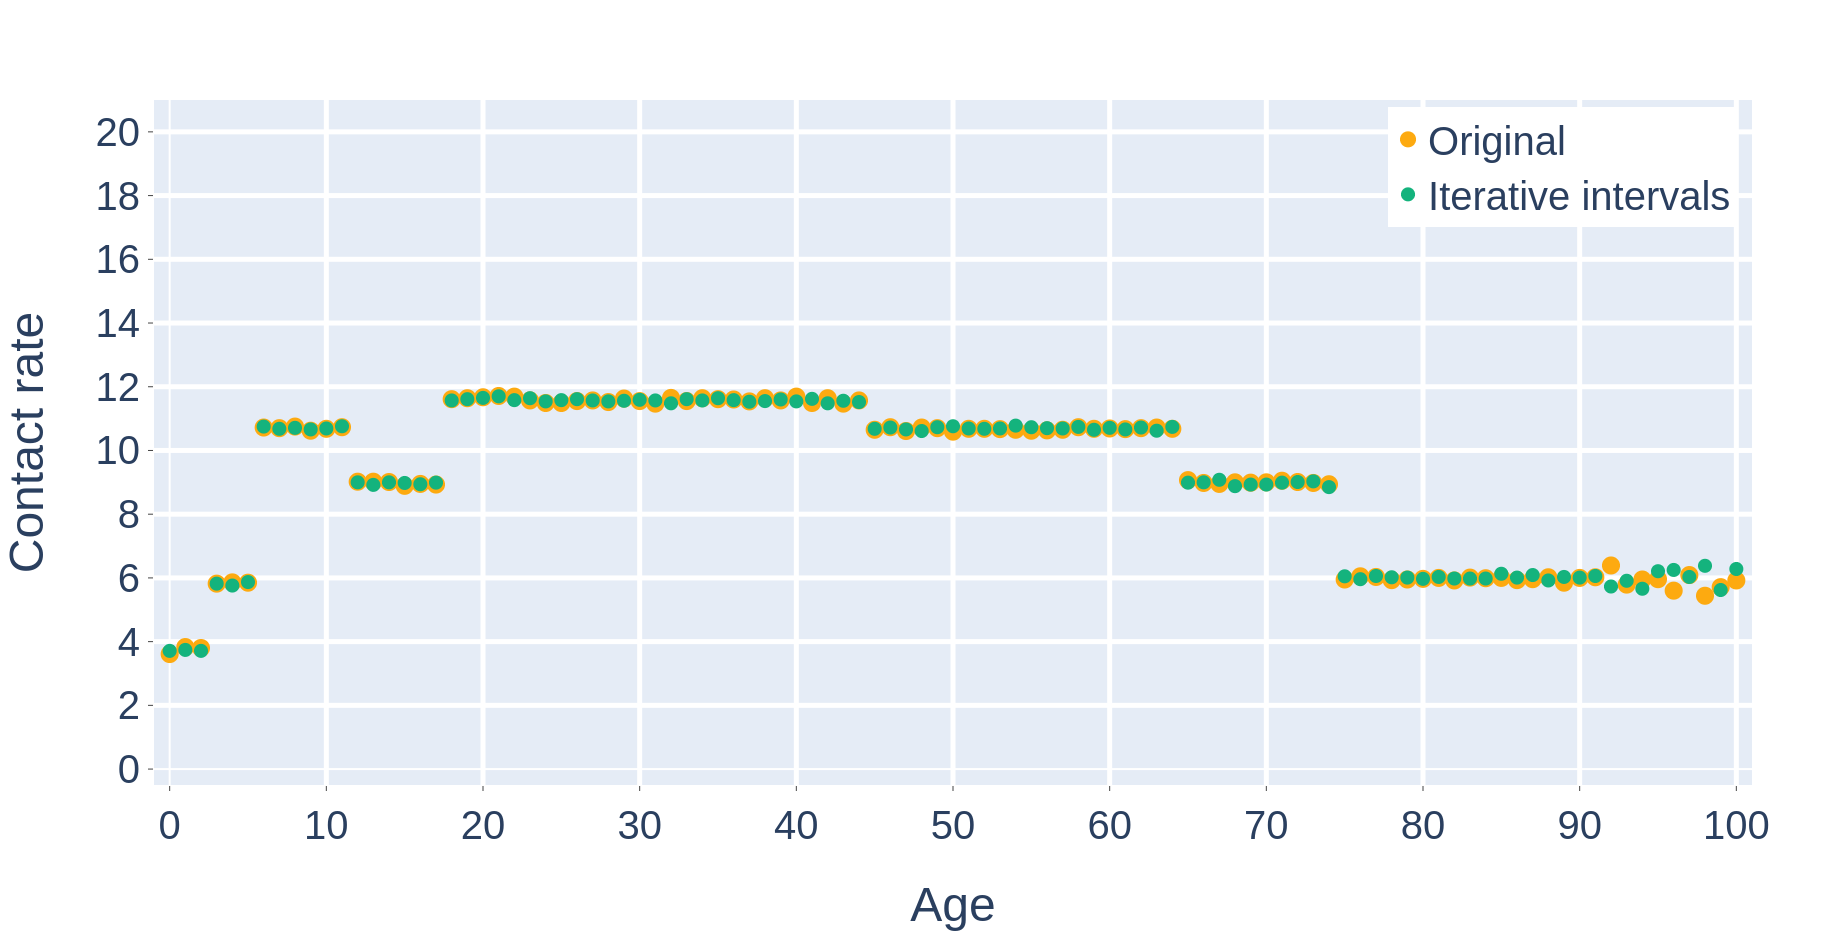
\includegraphics[width=\textwidth]{4 - Sampling/fig/iterative_intervals/ii_vs_standard_reverse_cr_primary.png}
        \caption{Primary community}
        \label{fig:ii_vs_standard_reversed_cr_standard_primary}
    \end{subfigure}
    \begin{subfigure}{.8\linewidth}
        \centering
        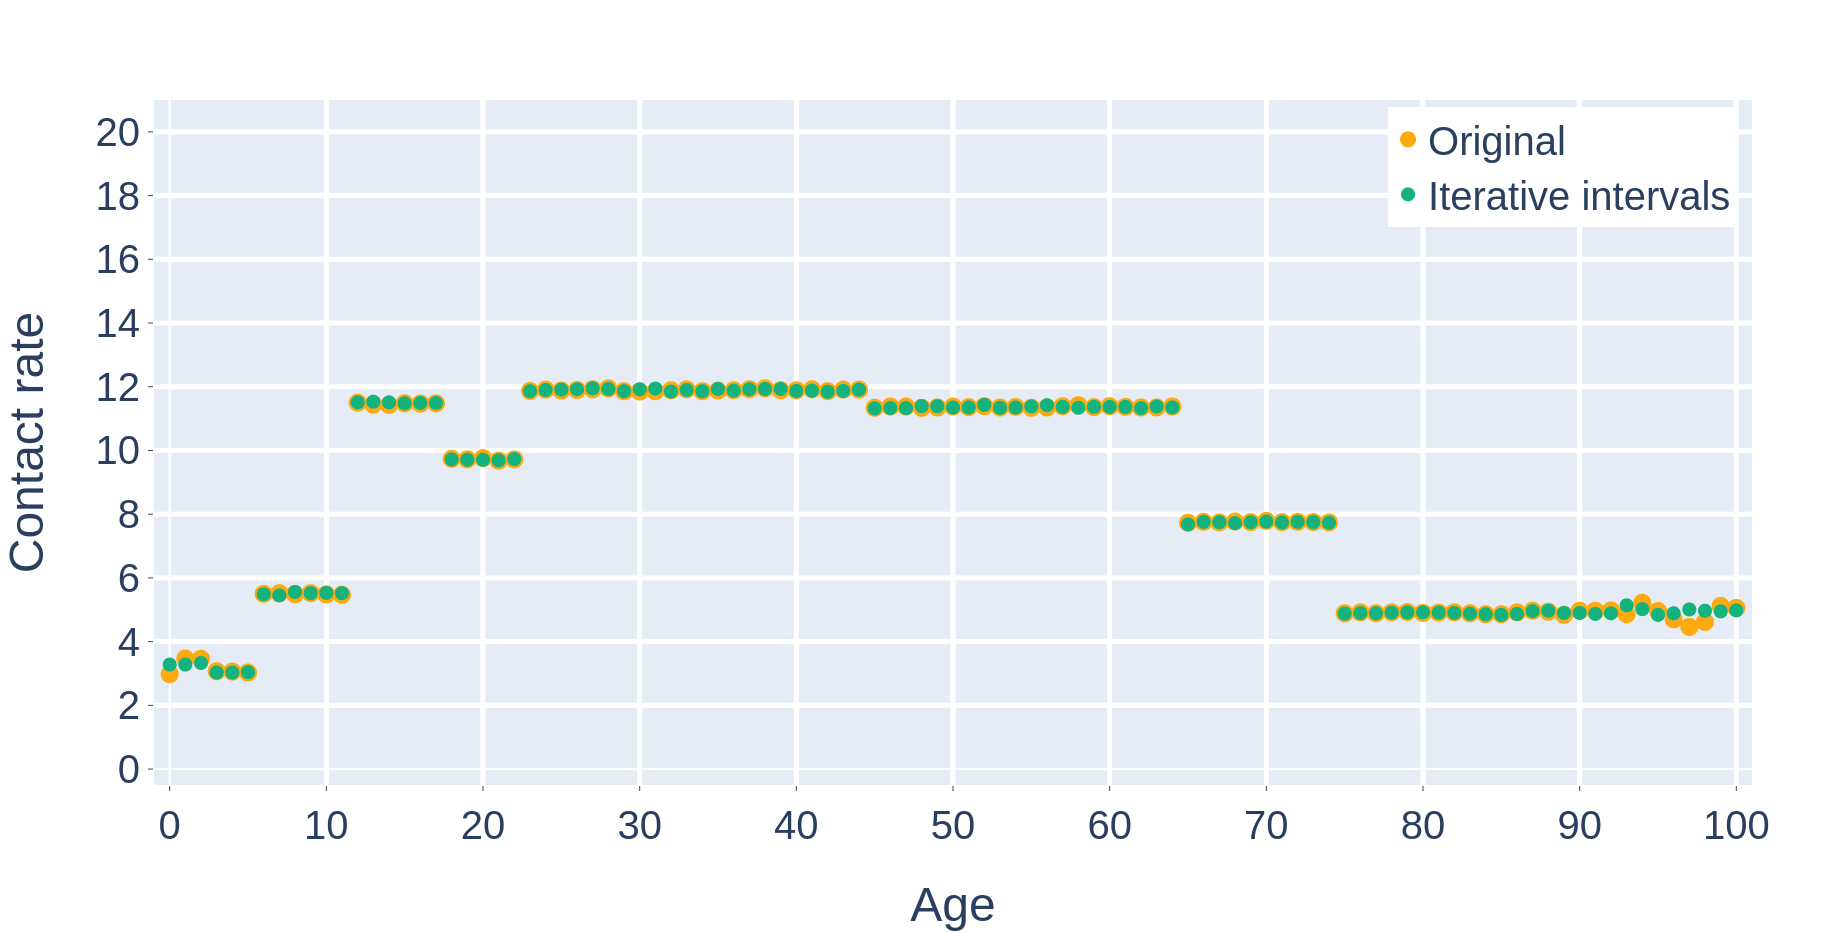
\includegraphics[width=\textwidth]{4 - Sampling/fig/iterative_intervals/ii_vs_standard_reverse_cr_secondary.png}
        \caption{Secondary community}
        \label{fig:ii_vs_standard_reversed_cr_standard_secondary}
    \end{subfigure}
    \caption{Comparison of the \textsc{Iterative-intervals} reversed contact rates with the original \textsc{All-to-All} reversed contact rates from Section \ref{subsec:reversed_contact_vector}.}
    \label{fig:ii_vs_standard_reverse_cr}
\end{figure}

\subsection{Performance}
\label{subsec:performance_iterative_intervals}
At last, we need to examine the \textsc{Iterative-intervals} approach to see if it is indeed an optimisation. The first performance test that we will discuss is the runtime of the infector, which is the vast majority of the total runtime in an \textsc{All-to-All} simulation. Figure \ref{fig:ii_vs_standard_infector} shows the infector runtimes of the \textsc{Iterative-intervals} approach compared to the original algorithm, which clearly indicates that our new approach is a big improvement. Table \ref{tab:ii_vs_standard_runtimes} confirms that we achieve an average speedup of 1.86 on the infector and 1.81 on the total simulation runtime.
\\\\
Next to the total runtime, we are also interested in how our optimisation affects the infector runtime regarding the pool type and size. In Section \ref{subsec:infector_runtimes} we showed how the average infector runtime has a quadratic curve in function of the pool size. Because the infector algorithm now works differently depending on the pool type, we need to examine the runtimes separately for every pool type. Figure \ref{fig:times_avg_ii} shows these average infector runtime results of the \textsc{Iterative-intervals} approach compared to the original algorithm. Here we can see that our new approach still has a quadratic curve, but that it becomes increasingly faster than the original the larger the pool. The differences for the K-12 school and college pool types are very little and will be discussed more in Section \ref{subsec:performance_sampling_with_iteration}.
\\\\
In Section \ref{subsec:infector_runtimes} we discussed the runtime of every pool type based on a 7-day week, which was also shown in Figure \ref{fig:standard_times_type_totals}. This taught us which pool types have a larger impact on the general runtime than others. Now we are only interested in how our approach affects the actual runtime of every pool type. Figure \ref{fig:ii_vs_standard_type_totals} shows the total runtimes for every pool type on an active day using different approaches, where we can see the impact of our approach on every pool type. The optimisations are most beneficial to the community pools and the workplace, while the household now takes more time to compute. This is due to the extra if-test in Algorithm \ref{alg:iterative_intervals} and is detrimental to its runtime. Altogether, the \textsc{Iterative-intervals} approach is a major optimisation for the \textsc{All-to-All} infector by only eliminating the amount of contact probability calculations.

\begin{figure}
    \centering
    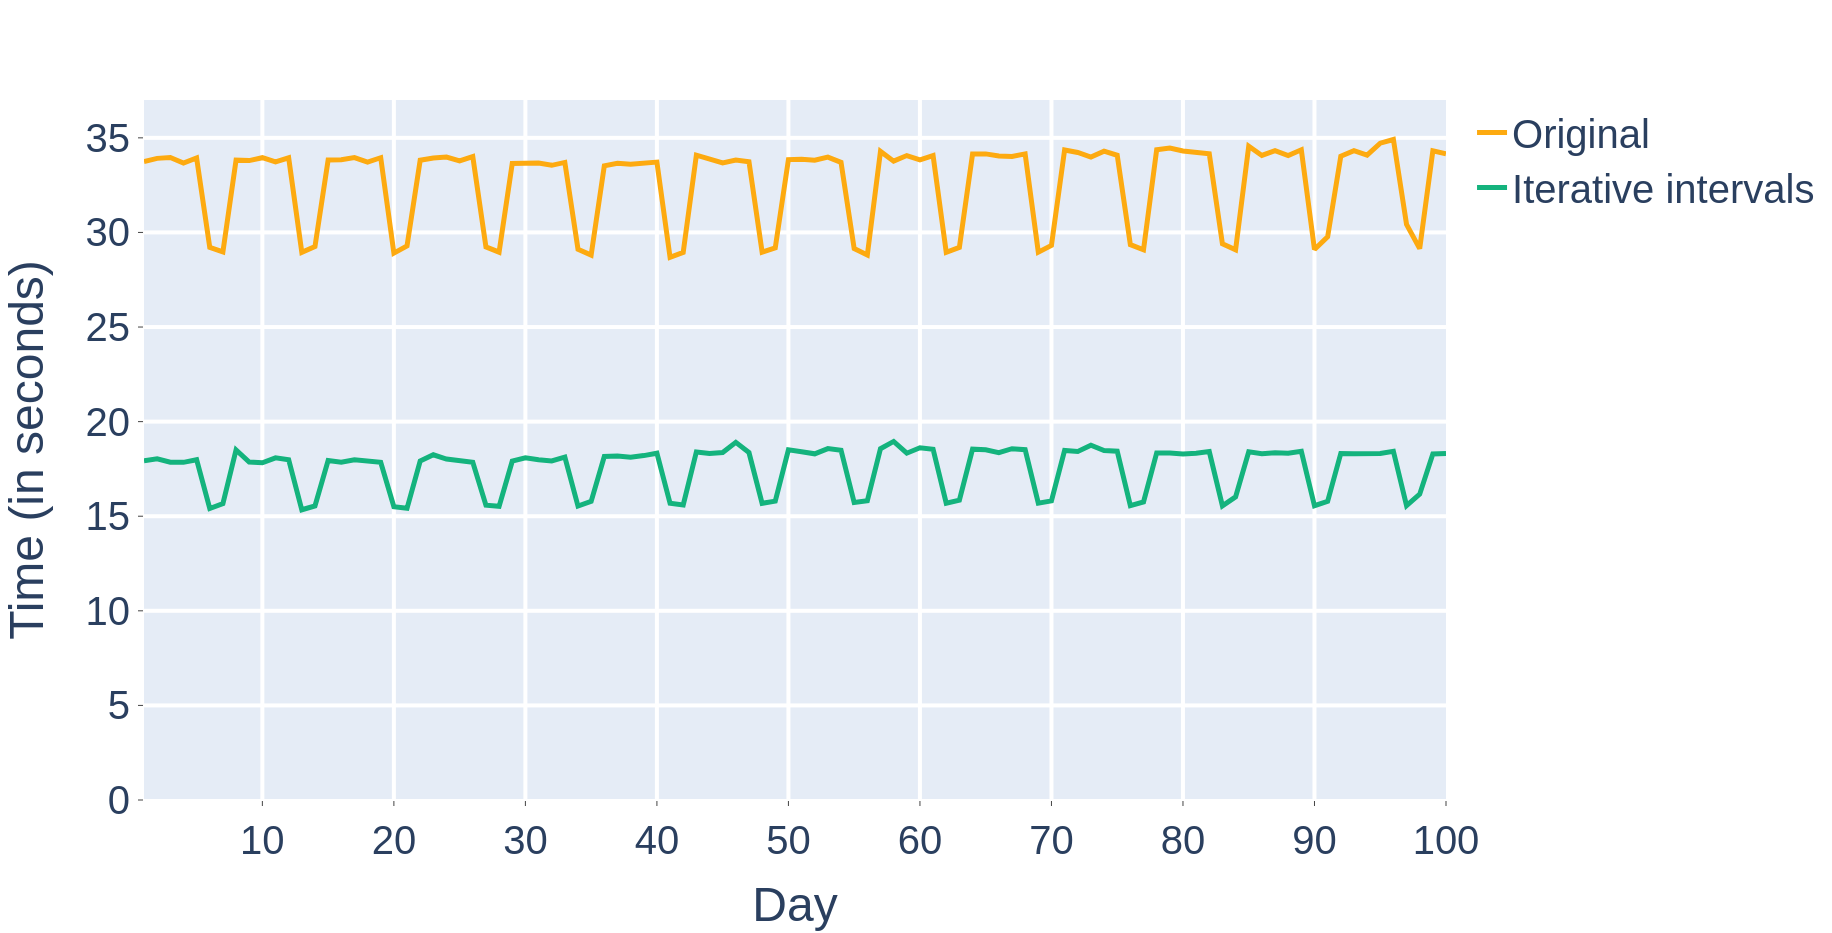
\includegraphics[width=\textwidth]{4 - Sampling/fig/iterative_intervals/ii_vs_standard_infector.png}
    \caption{Comparison of the infector runtimes between the original and \textsc{Iterative-intervals} approaches. Simulations run on 11M population for 100 days without holidays using 1 thread (configurations in Appendix \ref{appendix:configurations}).}
    \label{fig:ii_vs_standard_infector}
\end{figure}

\begin{table}
    \centering
    \begin{tabular}{@{}lrr@{}}
        \toprule
        \textsc{All-to-All} & Infector & Total \\ \midrule
        original & 32.63 & 33.77 \\
        iterative-intervals & 17.54 & 18.67 \\ \hdashline[1pt/1pt]
        speedup & 1.86 & 1.81 \\ \bottomrule
    \end{tabular}
    \caption{Comparison of the average daily runtimes between the original and \textsc{Iterative-intervals} approach. Simulations run on 11M population for 100 days without holidays using 1 thread (configurations in Appendix \ref{appendix:configurations}).}
    \label{tab:ii_vs_standard_runtimes}
\end{table}

\begin{figure}
    \centering
    \begin{subfigure}{.78\linewidth}
        \centering
        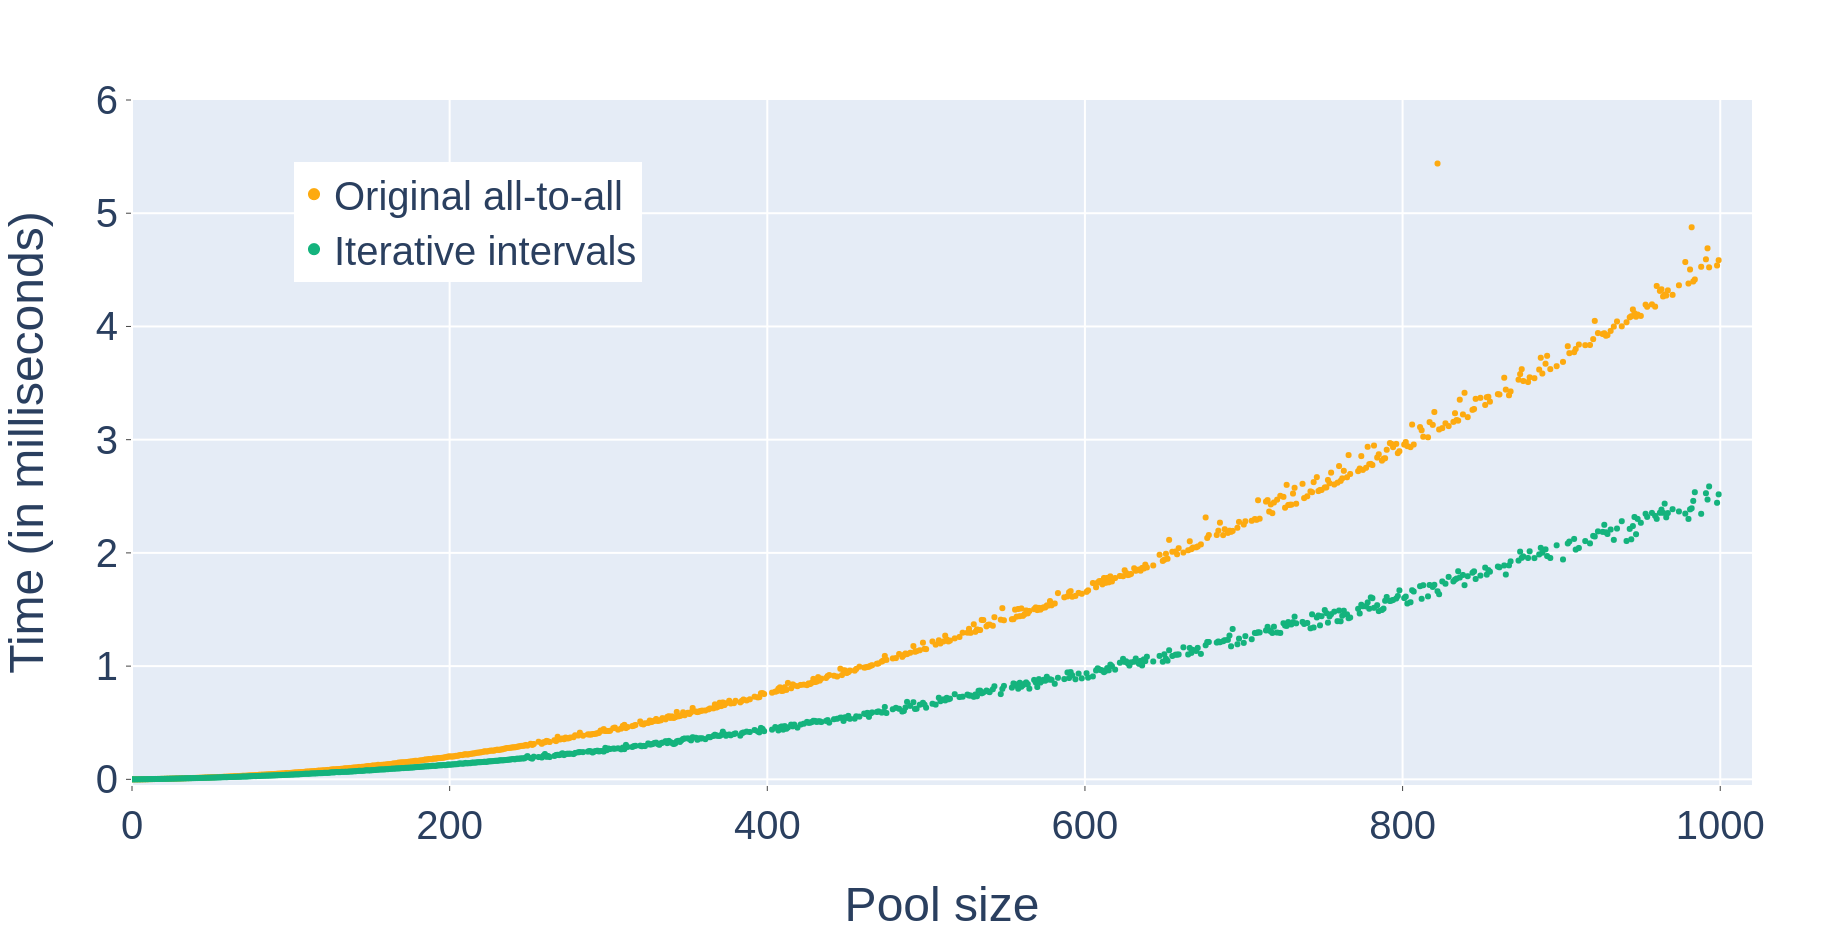
\includegraphics[width=\textwidth]{4 - Sampling/fig/iterative_intervals/times_avg_ii_workplace.png}
        \caption{Workplace}
        \label{fig:times_avg_ii_workplace}
    \end{subfigure}
    \begin{subfigure}{.78\linewidth}
        \centering
        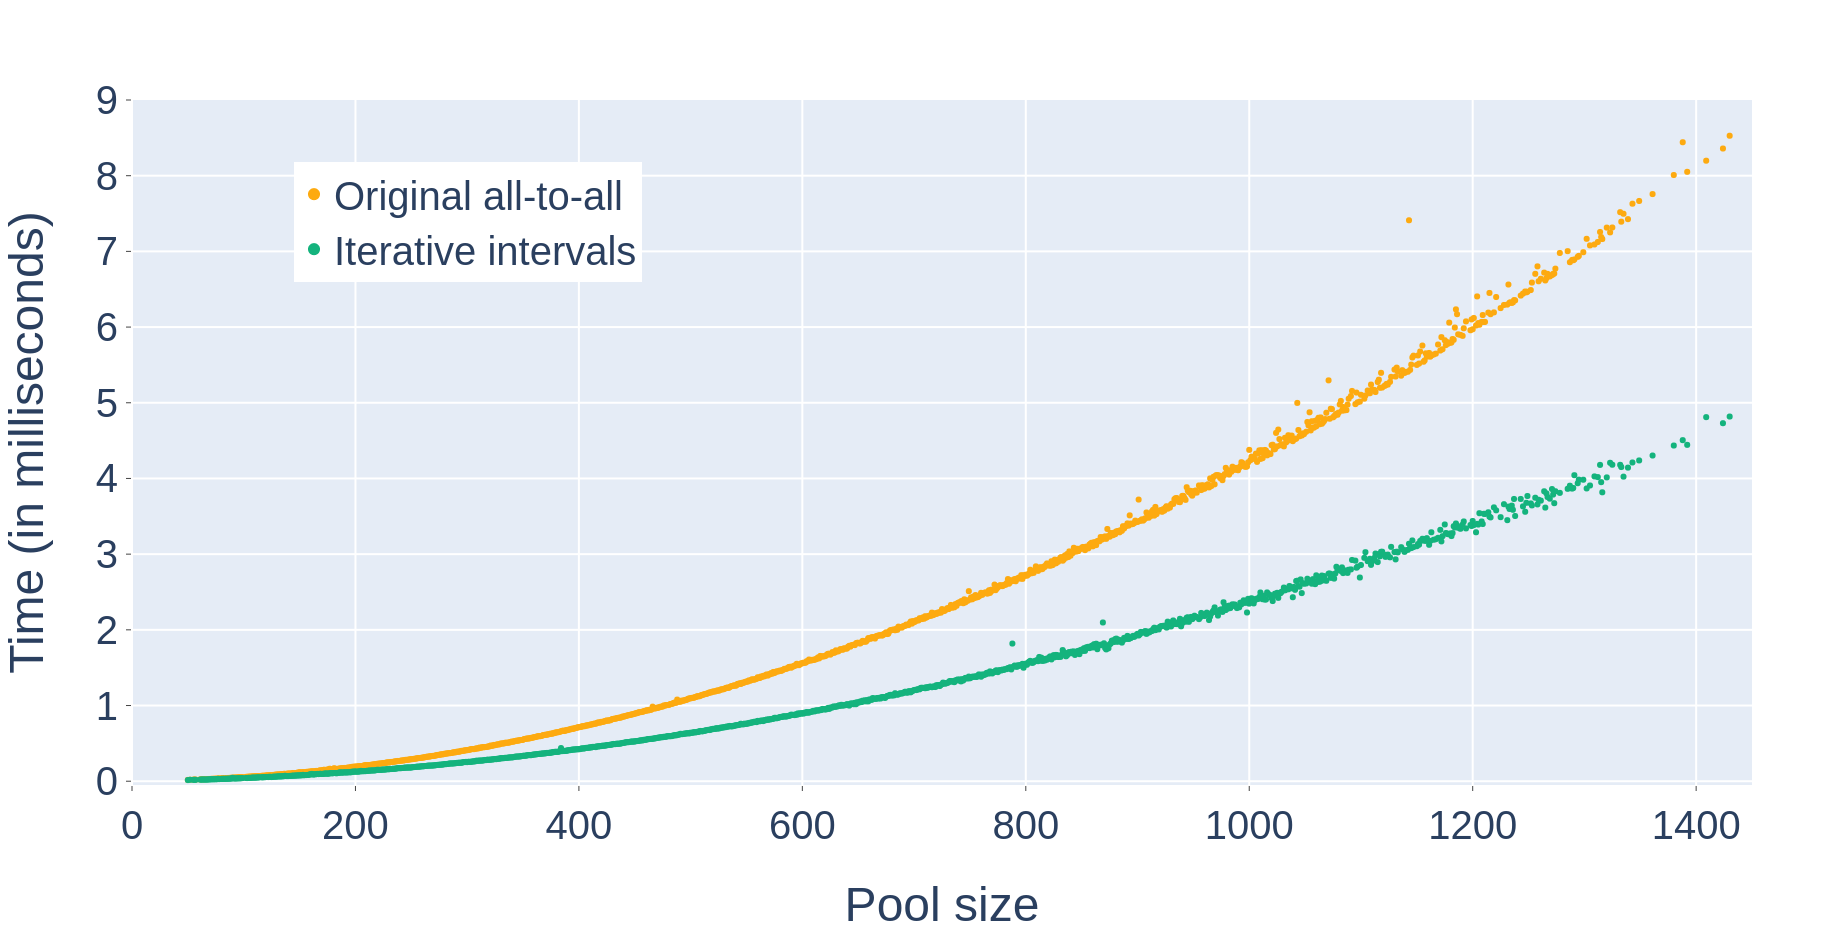
\includegraphics[width=\textwidth]{4 - Sampling/fig/iterative_intervals/times_avg_ii_primary.png}
        \caption{Primary community}
        \label{fig:times_avg_ii_primary}
    \end{subfigure}
    \begin{subfigure}{.78\linewidth}
        \centering
        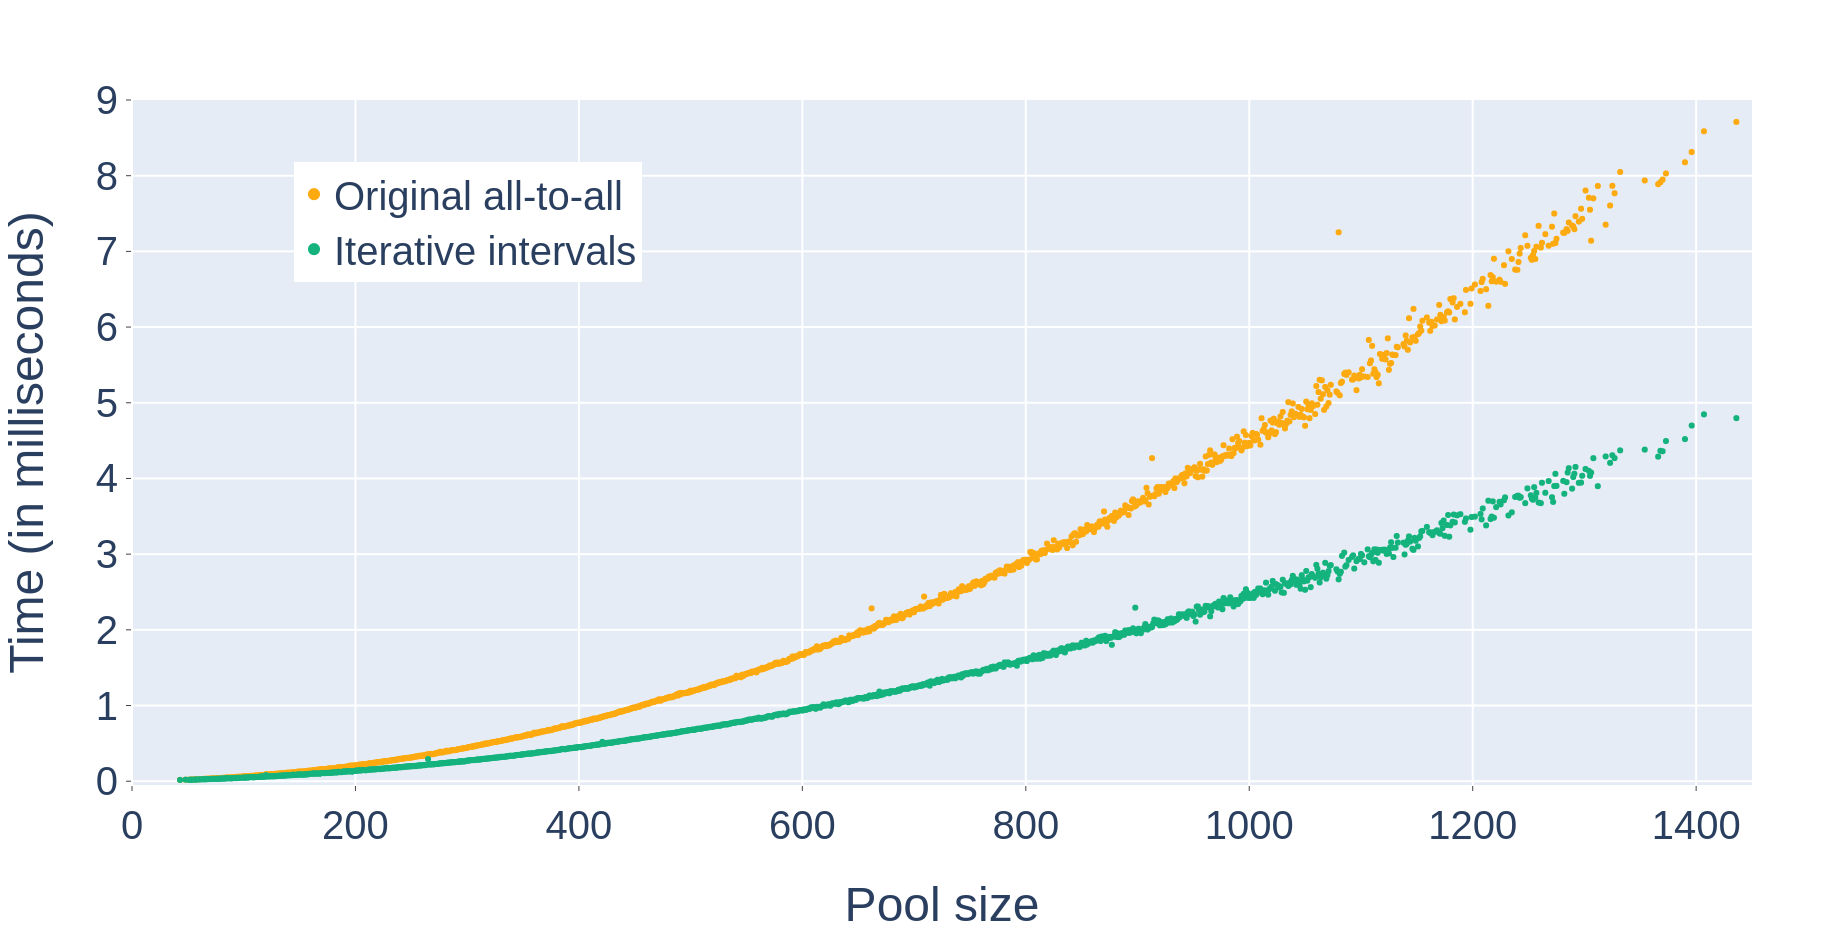
\includegraphics[width=\textwidth]{4 - Sampling/fig/iterative_intervals/times_avg_ii_secondary.png}
        \caption{Secondary community}
        \label{fig:times_avg_ii_secondary}
    \end{subfigure}
    \caption{Average infector runtimes (in milliseconds) per pool size using the original \textsc{All-to-All} and \textsc{Iterative-intervals}. Simulations run on 11M population for 100 days without holidays using 1 thread (configurations in Appendix \ref{appendix:configurations}).}
    \label{fig:times_avg_ii}
\end{figure}

\begin{figure}
    \centering
    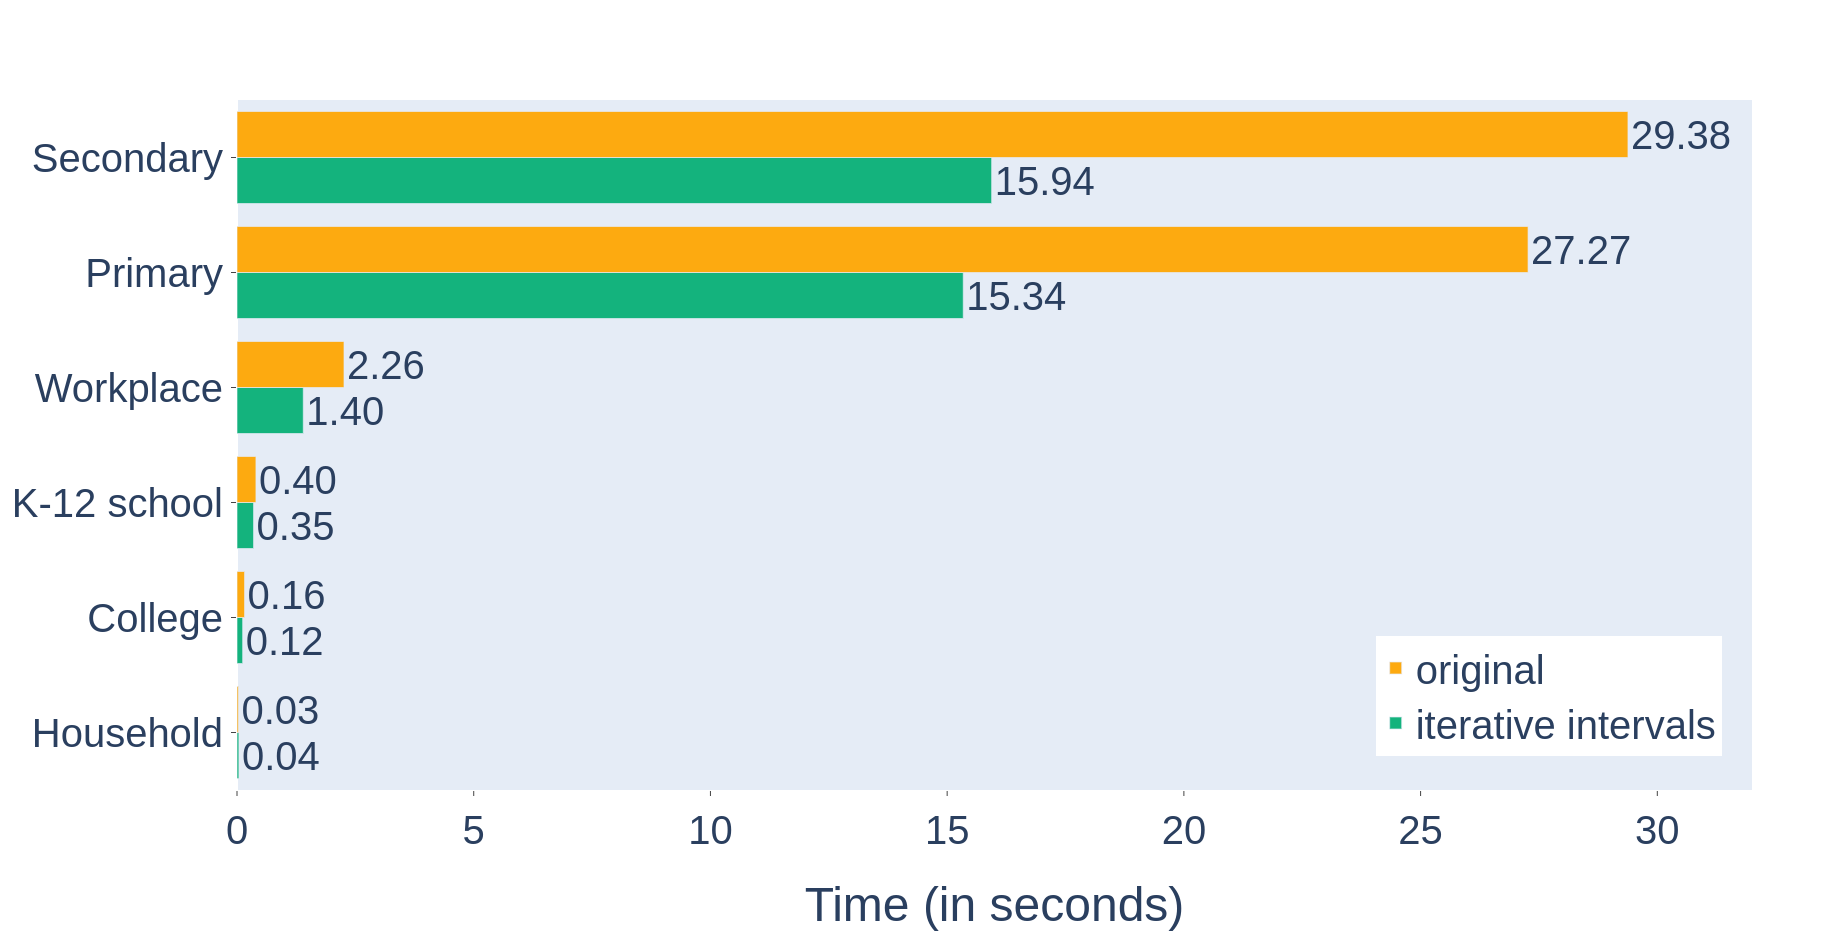
\includegraphics[width=\linewidth]{4 - Sampling/fig/iterative_intervals/ii_vs_standard_type_totals.png}
    \caption{Comparison of the total infector runtimes (in seconds) per pool type on a day in which its pools are active. Simulations run on 11M population for 100 days without holidays using 1 thread (configurations in Appendix \ref{appendix:configurations}).}
    \label{fig:ii_vs_standard_type_totals}
\end{figure}

\section{Sampling with iteration}
\label{sec:sampling_with_iteration}
Recall that the issue of our general sampling idea was the contact probability. For every member in a pool we want to calculate a sample size with a binomial distribution that needs to know the pool size and the probability. What we have learned from \textsc{Iterative-intervals} can now be used to implement the sampling idea. We again divide our pool in these intervals after which the intervals get compared in pairs. Then, we can calculate the sample size, which is the number of contacts that someone will have with the members in another interval. However, this raises a question about the contact calculations for members in the same interval. Calculating if two members have contact with each other happens only once, which is also the case for calculating contacts between two intervals. Every pair of intervals is only considered once to calculate the contacts between their members. If we now want to use the sampling approach for the members inside an interval, taking a sample for every member would cause the algorithm to consider two individuals twice. To avoid this problem, we will not use the sampling approach when comparing members in the same interval, but instead use the \textsc{Iterative-intervals} approach. Calculating contact for people in the same interval will thus calculate one contact probability and then compare everyone with everyone. Since our new approach uses sampling combined with the \textsc{Iterative-intervals}, we refer to it from now on as the \textsc{Sampling-with-iteration} approach.

\subsection{Implementation}
\label{subsec:implementation_sampling_with_iteration}
The pseudo code of the \textsc{Sampling-with-iteration} approach is given in Algorithm \ref{alg:sampling_with_iteration}. Just like the \textsc{Iterative-intervals}, the household type pools still use the original \textsc{All-to-All} method because their maximum size is six individuals, while the rest of the pools start off with dividing their members in the age intervals. Then, all of the intervals get compared once with each other. Like we said, the contacts between the people in the same interval are calculated in the \textsc{Iterative-intervals} way, where a double for-loop compares everyone with each other and only one contact probability is calculated for all of them. The comparisons with the other intervals work by iterating over the members of one interval, where for every person $P_{1}$ a sample size gets calculated by the binomial distribution based on the number of people in the other interval, $interval_{2}$, and the contact probability between the members of the two intervals. This sample size indicates the number of people from $interval_{2}$ that $P_{1}$ will have contact with. If the sample size is zero we can just skip $P_{1}$ and continue to the next one, because there are no contacts for the current $P_{1}$ with members in $interval_{2}$. If the sample size is equal to the number of people in $interval_{2}$, it means that $P_{1}$ will have contact with everyone in the interval. When this happens, we do not need to sample and can just iterate over the entire interval and handle the contacts and transmissions between $P_{1}$ and everyone in $interval_{2}$. If the sample size is smaller than the size of $interval_{2}$, we need to determine who will have contact with $P_{1}$. To select these contacts, we `draw' a person from $interval_{2}$ based on a random number. If this randomly selected individual is present in the pool and if we have not already drawn him for the same $P_{1}$, we register their contact and calculate the transmission as we know.

\begin{algorithm}
\caption{Pseudo code of the \textsc{Sampling-with-iteration} infector.}
\label{alg:sampling_with_iteration}
\begin{algorithmic}[1]
    \Require{$P_{1} \dots P_{N}$, $type$} \Comment{All members of the pool and type of pool}\;
    \Statex
    \If{$type = household$}
        \State original \textsc{All-to-All} \Comment{Algorithm \ref{alg:all-to-all}}
    \Else
        \State $S[\;] \gets$ \Call{sort\_intervals}{$P[\;], type$}\Comment{Algorithm \ref{alg:age_sorting}, returns interval sizes}
        \State $N_{intervals} \gets$ \Call{sizeof}{$S[\;]$} \Comment{Number of intervals}
        \Statex
        \For{$interval_{1} \gets 1$ to $N_{intervals}$} \Comment{Iterate intervals}
            \For{$interval_{2} \gets interval_{1}$ to $N_{intervals}$} \Comment{Iterate remaining intervals}
                \State $C_{prob} \gets$ \Call{contact\_probability}{$interval_{1}, interval_{2}$} \Comment{Algorithm \ref{alg:contact_probability}}
                \Statex
                \If{$interval_{1} = interval_{2}$}
                    \State \textsc{Iterative-intervals} \Comment{Algorithm \ref{alg:iterative_intervals}}
                \Else
                    \Foreach{member $P_{1}$ in $interval_{1}$}
                        \If{$P_{1}$ not in pool}
                            \State continue to next $P_{1}$
                        \EndIf
                        \State $sample \gets$ \Call{binomial}{$S[interval_{2}], C_{prob}$} \Comment{Binomial distribution}
                        \If{$sample$ = 0}
                            \State continue to next $P_{1}$
                        \ElsIf{$sample$ = $S[interval_{2}]$}
                            \State iterate over $interval_{2}$ and register contact with everyone
                        \Else
                            \State $draws_{all} \gets 0$ \Comment{Number of draws}
                            \State $draws_{good} \gets 0$ \Comment{Number of good draws}
                            \State $drawn\_members \gets [\;]$
                            \Statex
                            \While{$draws_{good} < sample$ AND $draws_{all} < S[interval_{2}]$}
                                \State $P_{2} \gets$ random member of $interval_{2}$
                                \If{$P_{2}$ in $drawn\_members$}
                                    \State draw next $P_{2}$
                                \EndIf
                                \State add $P_{2}$ to $drawn\_members[\;]$
                                \State $++draws_{all}$
                                \If{$P_{2}$ not in pool}
                                    \State draw next $P_{2}$
                                \EndIf
                                \State $++draws_{good}$
                                \State register contact
                                \If{$P_{1}$ or $P_{2}$ susceptible and other infectious}
                                    \State $T_{prob} \gets$ transmission probability
                                    \If{\Call{BernoulliTrial}{$T_{prob}$}}
                                        \State infect the susceptible one
                                    \EndIf
                                \EndIf
                            \EndWhile
                        \EndIf
                    \EndForeach
                \EndIf
            \EndFor
        \EndFor
    \EndIf
\end{algorithmic}
\end{algorithm}

\subsection{Correctness}
\label{subsec:correctness_sampling_with_iteration}
Again we need to make sure that this approach is also correct. The first step is to run the built-in testing tool to see if the results, such as the number of infected people, lie within a certain interval and that it can also be used with parallellization. The \textsc{Sampling-with-iteration} algorithm passed this test, so we then continue to compute the reversed contact vectors, which are displayed in Figure \ref{fig:swi_vs_standard_reversed_cr}. The reversed rates of the original \textsc{All-to-All} algorithm are very similar to the reversed rates of the \textsc{Sampling-with-iteration} approach. Because this new approach passed both tests, we conclude that it is a valid \textsc{All-to-All} algorithm.

\begin{figure}
    \centering
    \begin{subfigure}{.8\linewidth}
        \centering
        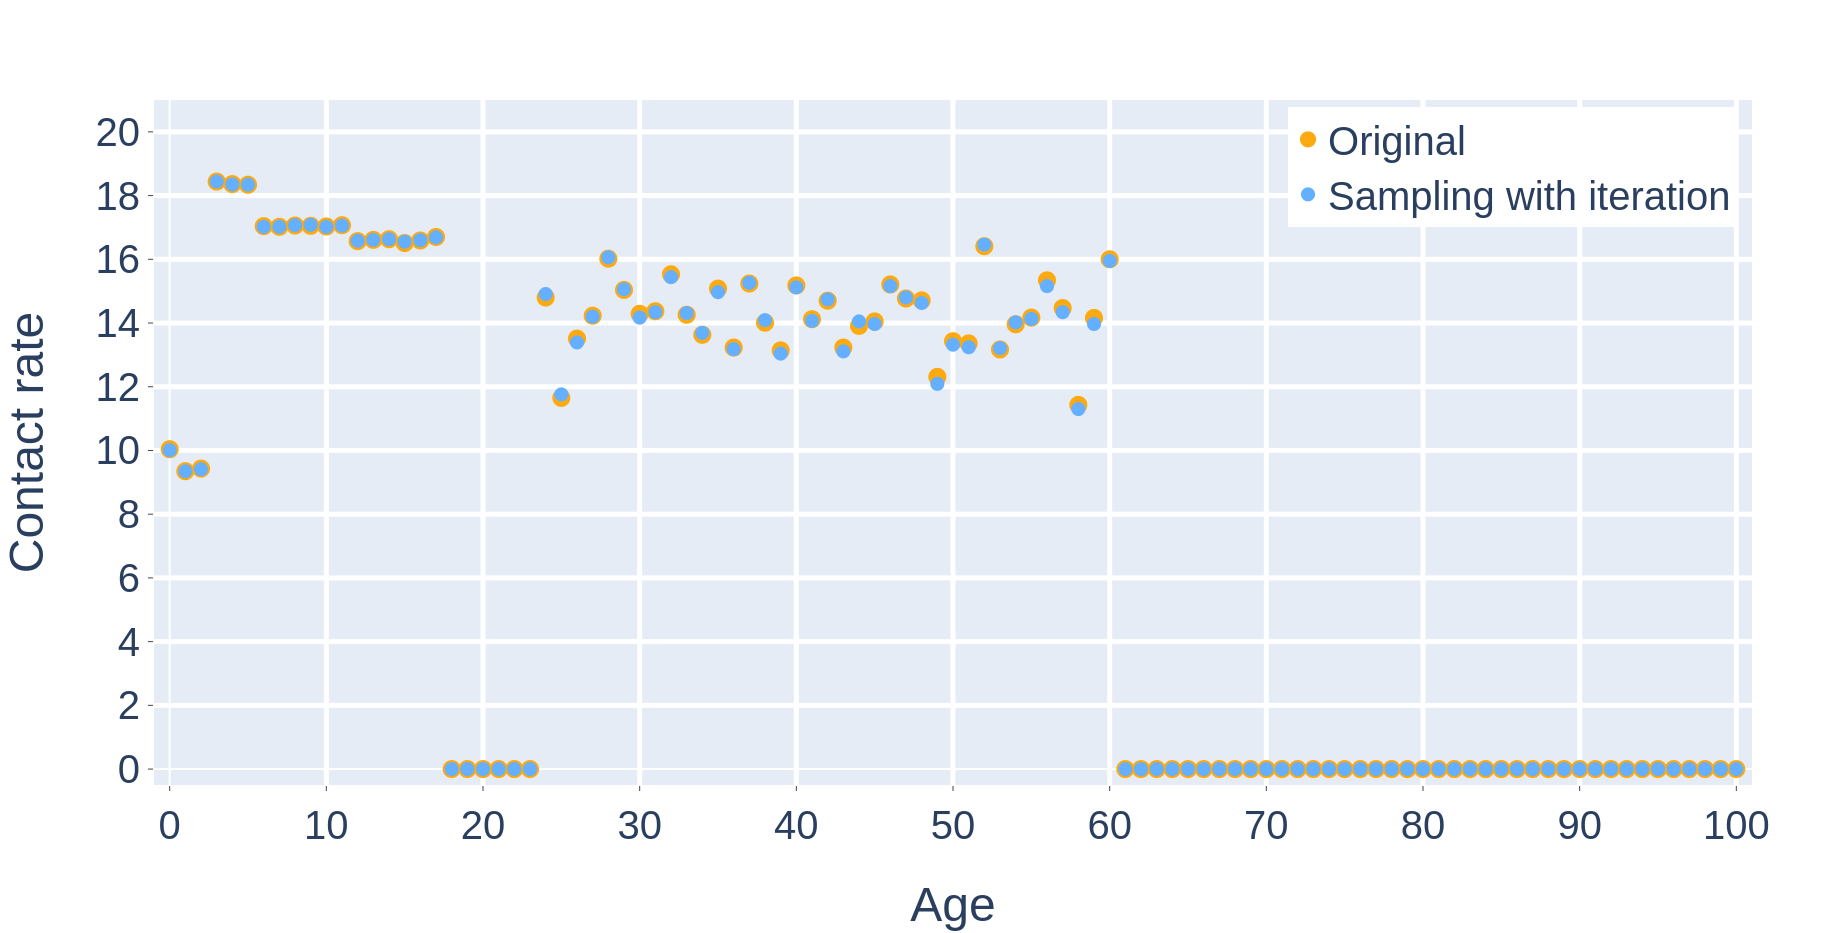
\includegraphics[width=\textwidth]{4 - Sampling/fig/sampling_with_iteration/swi_vs_standard_reverse_cr_k12school.png}
        \caption{K-12 school}
        \label{fig:swi_vs_standard_reversed_cr_k12school}
    \end{subfigure}
    \begin{subfigure}{.8\linewidth}
        \centering
        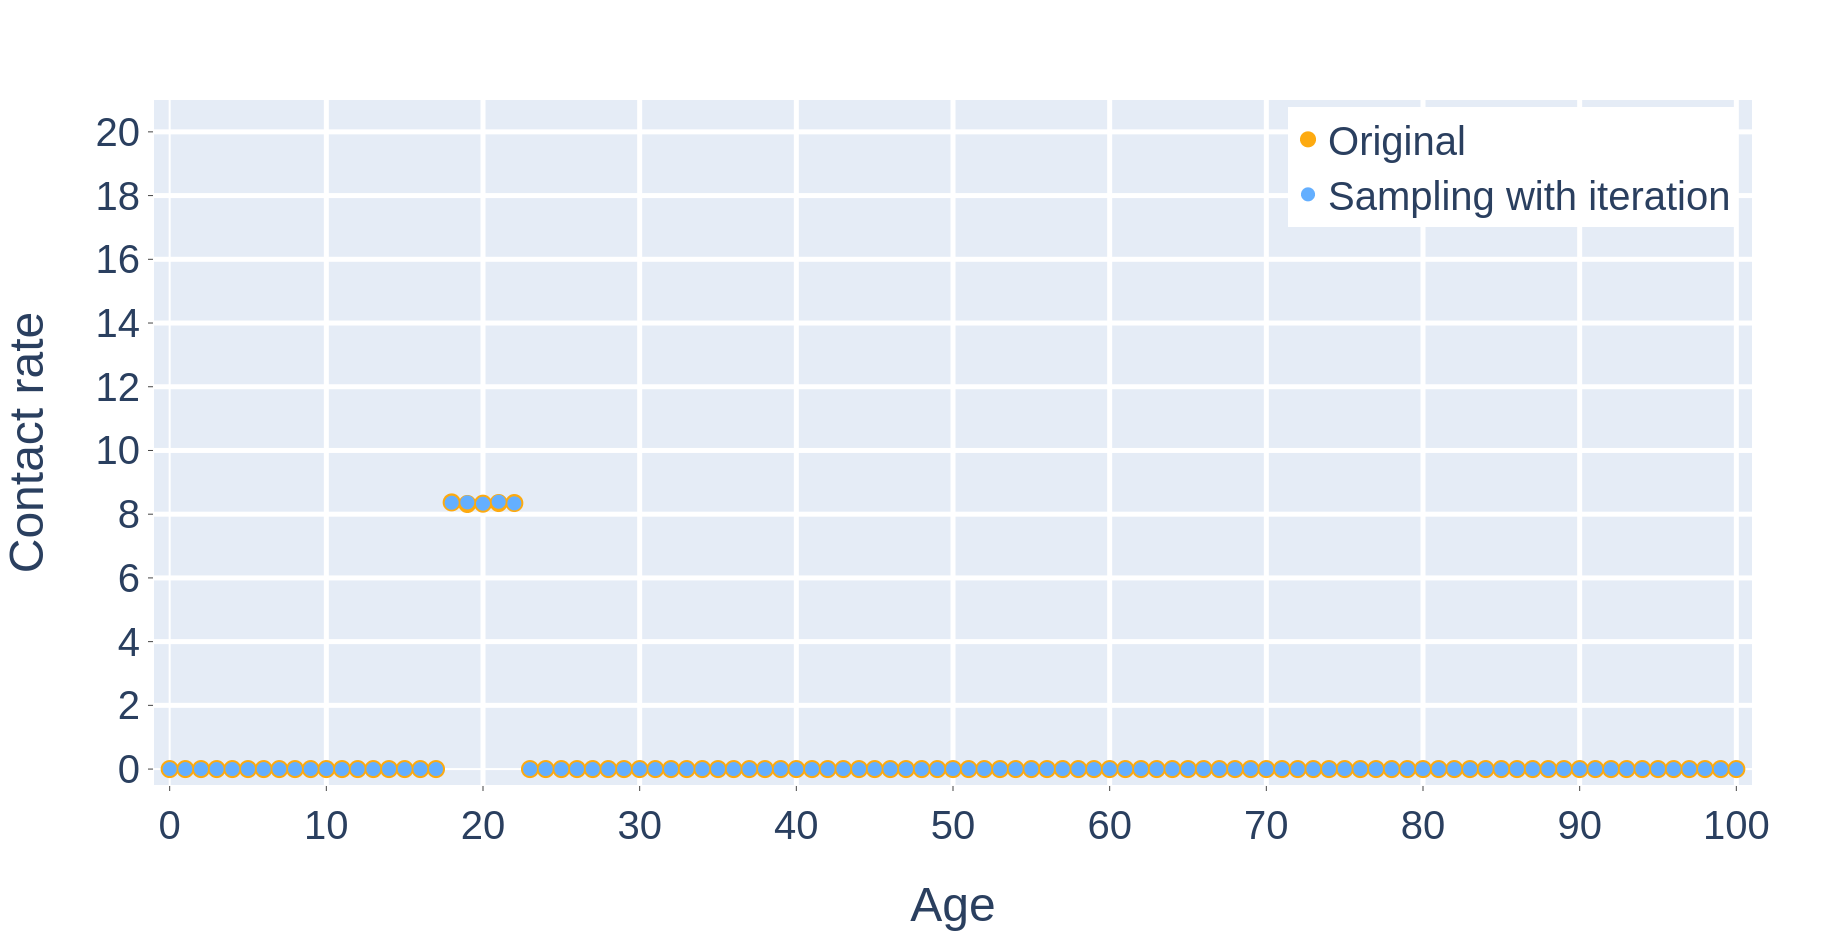
\includegraphics[width=\textwidth]{4 - Sampling/fig/sampling_with_iteration/swi_vs_standard_reverse_cr_college.png}
        \caption{College}
        \label{fig:swi_vs_standard_reversed_cr_college}
    \end{subfigure}
    \begin{subfigure}{.8\linewidth}
        \centering
        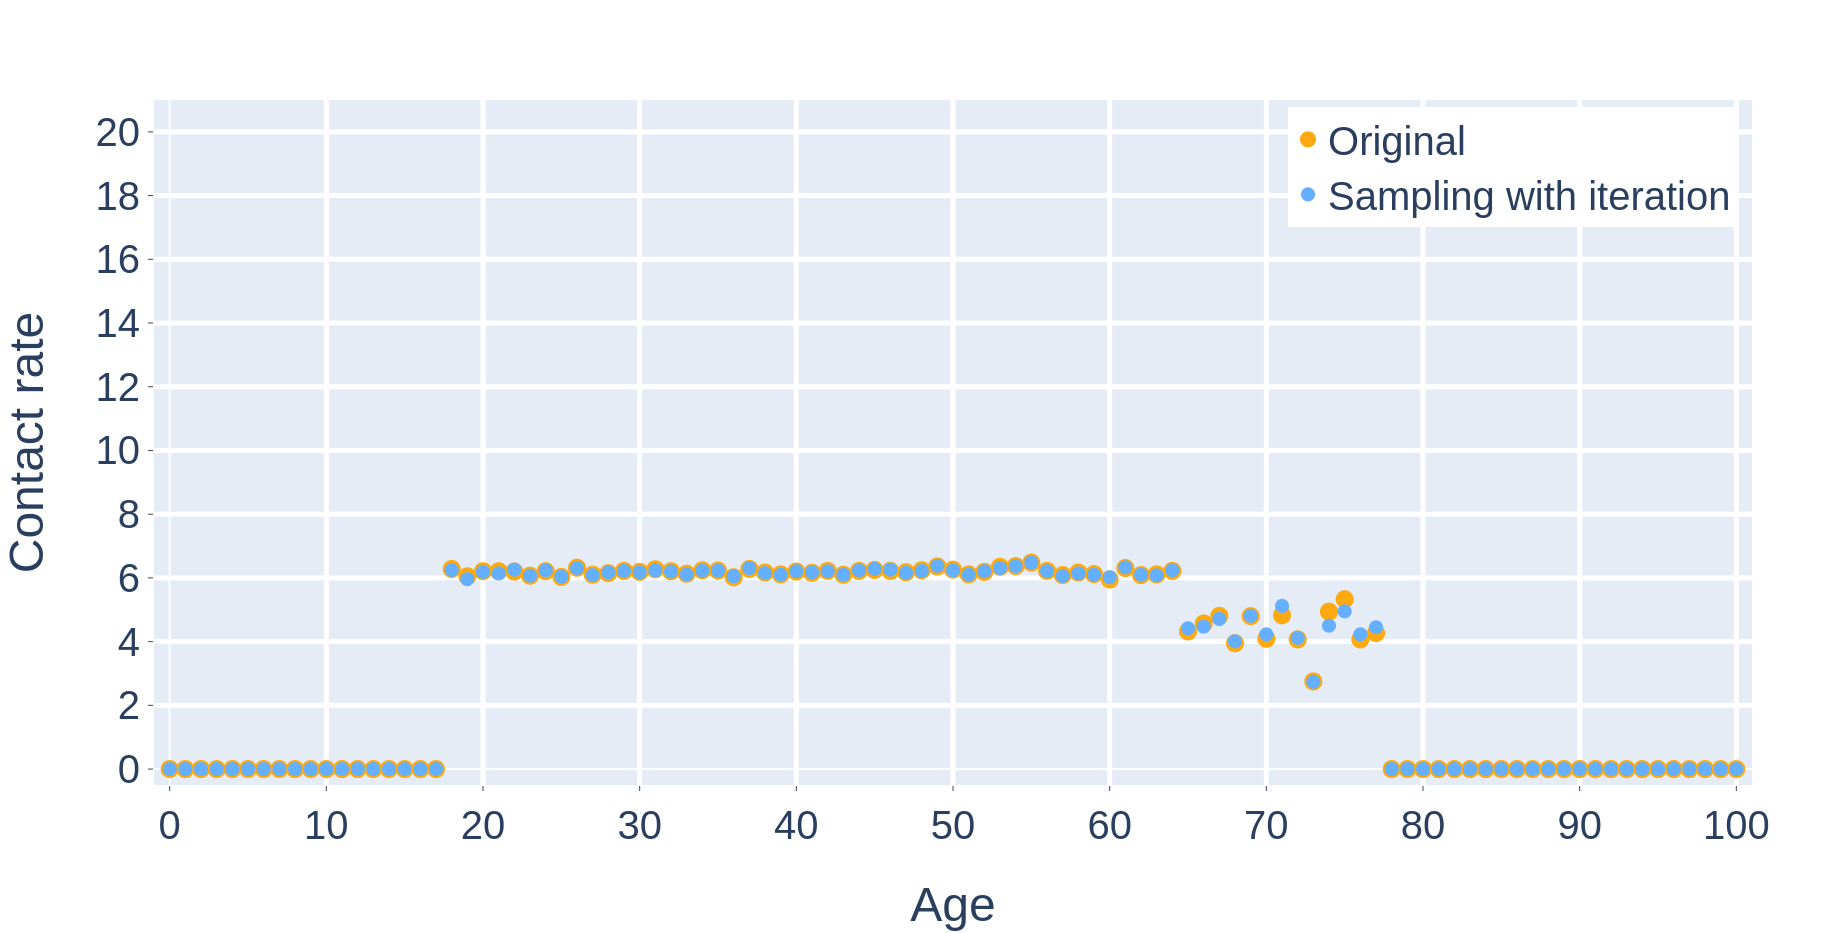
\includegraphics[width=\textwidth]{4 - Sampling/fig/sampling_with_iteration/swi_vs_standard_reverse_cr_workplace.png}
        \caption{Workplace}
        \label{fig:swi_vs_standard_reversed_cr_workplace}
    \end{subfigure}
    \caption{Comparison of the \textsc{Sampling-with-iteration} reversed contact rates with the original \textsc{All-to-All} reversed contact rates from Section \ref{subsec:reversed_contact_vector}.}
\end{figure}
\begin{figure}\ContinuedFloat
    \centering
    \begin{subfigure}{.8\linewidth}
        \centering
        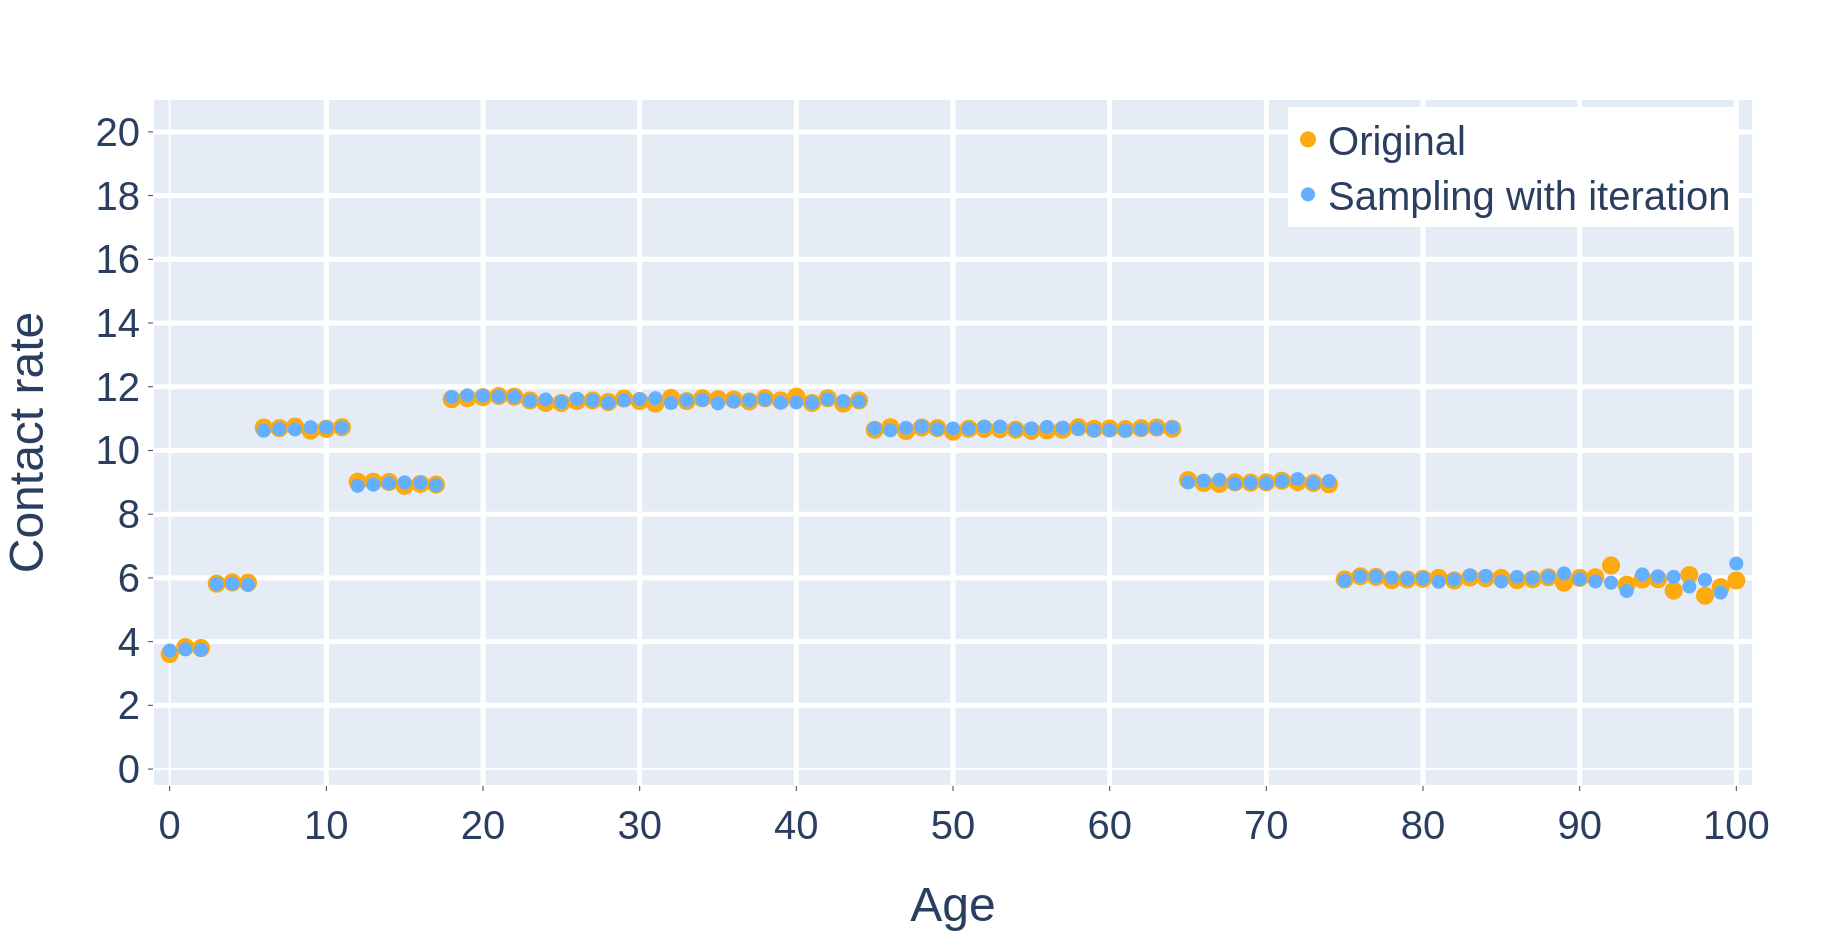
\includegraphics[width=\textwidth]{4 - Sampling/fig/sampling_with_iteration/swi_vs_standard_reverse_cr_primary.png}
        \caption{Primary community}
        \label{fig:swi_vs_standard_reversed_cr_primary}
    \end{subfigure}
    \begin{subfigure}{.8\linewidth}
        \centering
        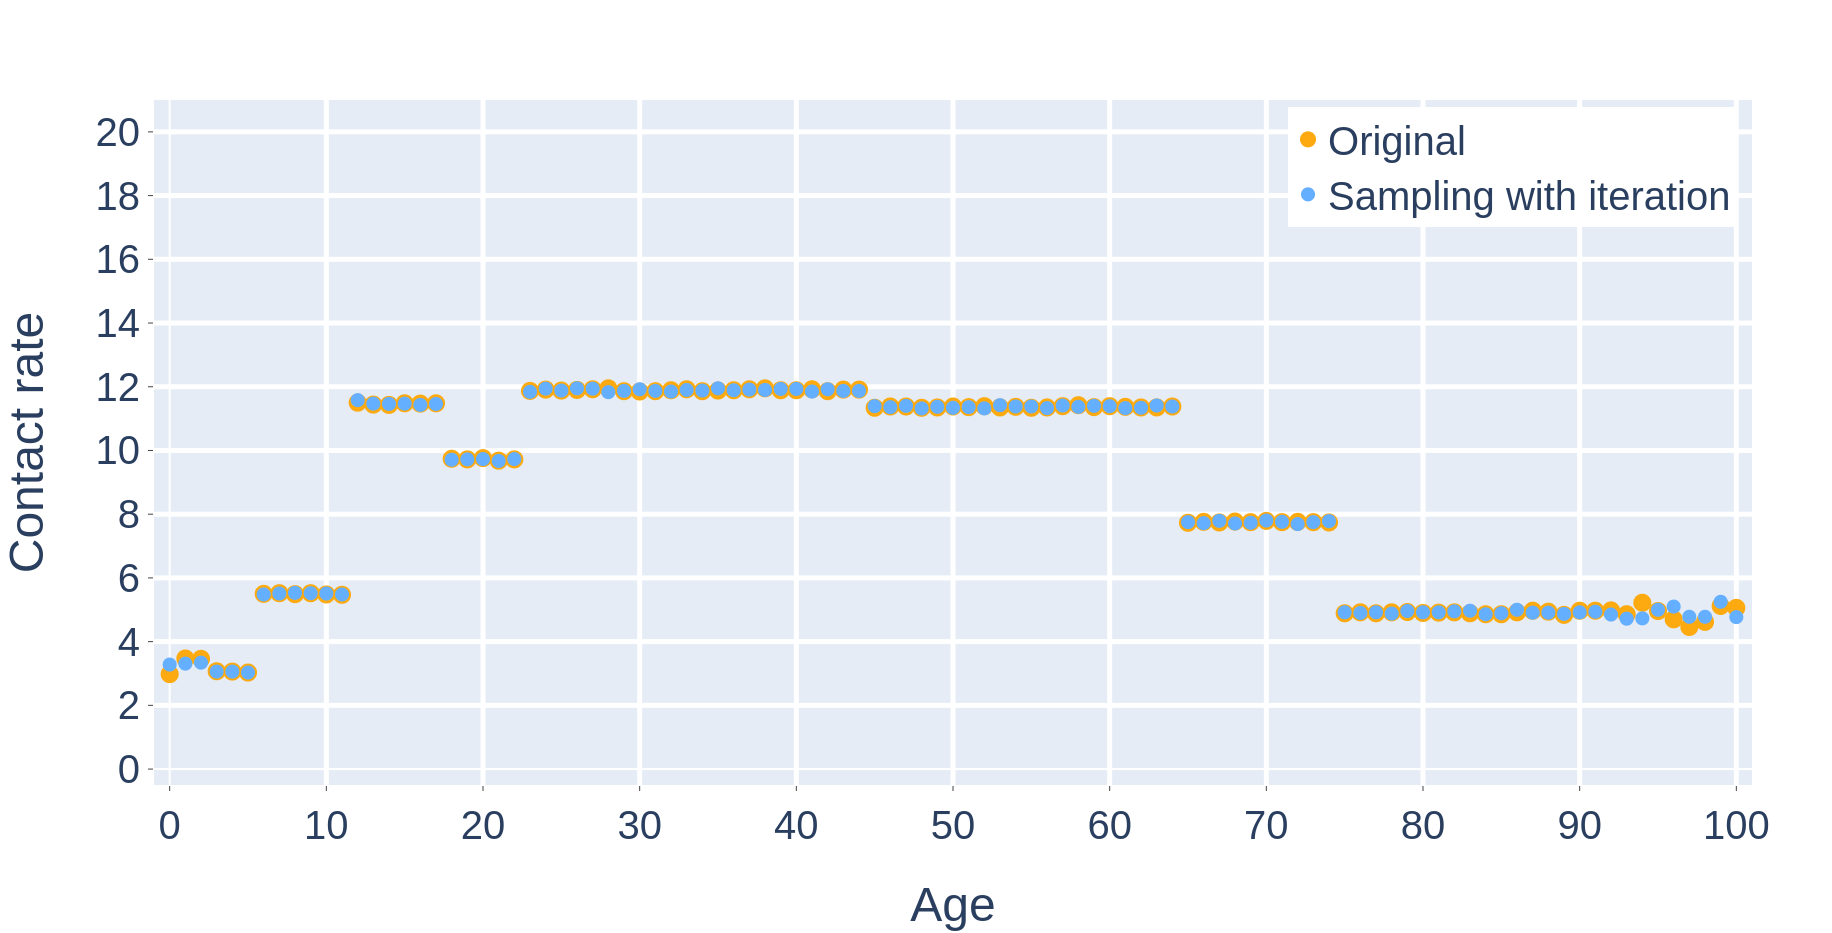
\includegraphics[width=\textwidth]{4 - Sampling/fig/sampling_with_iteration/swi_vs_standard_reverse_cr_secondary.png}
        \caption{Secondary community}
        \label{fig:swi_vs_standard_reversed_cr_secondary}
    \end{subfigure}
    \caption{Comparison of the \textsc{Sampling-with-iteration} reversed contact rates with the original \textsc{All-to-All} reversed contact rates from Section \ref{subsec:reversed_contact_vector}.}
    \label{fig:swi_vs_standard_reversed_cr}
\end{figure}

\subsection{Performance}
\label{subsec:performance_sampling_with_iteration}
Now that we have verified the correctness of \textsc{Sampling-with-iteration}, we want to know how it performs compared to our other two approaches. Figure \ref{fig:swi_vs_rest_infector} shows the total infector runtime per day for the different algorithms, which proves that \textsc{Sampling-with-iteration} is even faster than \textsc{Iterative-intervals}. Table \ref{tab:swi_vs_standard_runtimes} reveals that our latest algorithm achieves an average total speedup of 2.33, which is due to the 2.47 average speedup in the infector.
\\\\
Our general idea from Section \ref{sec:general_idea} explains that the improvements we want to make will have the most impact on the larger pools because of the linear time complexity. Hence, Figure \ref{fig:times_avg_swi_pType_full} shows the average infector runtime regarding the pool size for the workplace and community pools. The community pools show that our \textsc{Sampling-with-iteration} approach has a somewhat linear curve, as we would expect, and that it is therefore a massive optimisation the larger the pool size. However, Figure \ref{fig:times_avg_swi_pType_workplace_full} shows that the workplace pools have a quadratic curve, similar to the \textsc{Iterative-intervals} algorithm. This is because the workplace has only three different age intervals where the [0,18]-interval is empty on most occasions. Secondly, almost everyone resides in the [19,65]-interval according to the workplace age distribution in Figure \ref{fig:workplace_age_distribution}. This causes workplace pools to spend most of their time calculating contacts between people in the same interval, which uses the \textsc{Iterative-intervals} method. \textsc{Sampling-with-iteration} has thus barely any effect on the workplace contact calculations. The community pools have nine different intervals that are all evenly distributed, which supports this explanation.
\\\\
The impact of our optimisation for every pool type is presented in Figure \ref{fig:swi_vs_rest_type_totals}, which shows that the community pools are the only ones that benefit from our new algorithm. The rest of the pools are all slower than the \textsc{Iterative-intervals} or even the original \textsc{All-to-All} approach. To further investigate this, a more detailed view on these pools is needed. Figure \ref{fig:times_avg_swi_pType} displays the average infector runtimes only for the pools that contain 300 people or less. The primary community in Figure \ref{fig:times_avg_swi_pType_primary}, as well as the secondary community in Figure \ref{fig:times_avg_swi_pType_secondary}, both show that the \textsc{Sampling-with-iteration} has the worst results for smaller pools. The reason for this is that the algorithm has extra overhead because of the binomial distribution calculation and the random member draws. When the intervals contain only a few individuals, the overhead takes more time than simply comparing everyone with everyone like the \textsc{Iterative-intervals} method does. Only pools with around 275 people achieve the fastest time with the \textsc{Sampling-with-iteration} approach, but it is already faster than the original one for pools with a size of at least 150 individuals. Figures \ref{fig:times_avg_swi_pType_k12school} and \ref{fig:times_avg_swi_pType_college} also show that the K-12 school and college pools lose speed using \textsc{Sampling-with-iteration}, for which the reason is also the predominant overhead in smaller pools and intervals.
\\\\
In the end we can conclude that our \textsc{Sampling-with-iteration} algorithm is a major optimisation compared to the original and \textsc{Iterative-intervals} \textsc{All-to-All} algorithms for larger pools. The time complexity of this algorithm is hard to define, because it is not completely linear due to the contact calculations between people in the same interval which still has a quadratic time complexity. Also, a double for-loop is used to iterate over the intervals which also results a quadratic time complexity in function of the number of intervals. However, this is negligible if there are not that many intervals as is the case for our different pool types. Altogether, this new approach is more efficient the larger the pools, as long as their members can be somewhat evenly divided in multiple age intervals.
\\\\
A possible solution to the workplace runtimes, could be to divide the large intervals into multiple smaller ones. We chose to not further investigate this, because we want to present general algorithms where every pool uses the same approach.

\begin{figure}
    \centering
    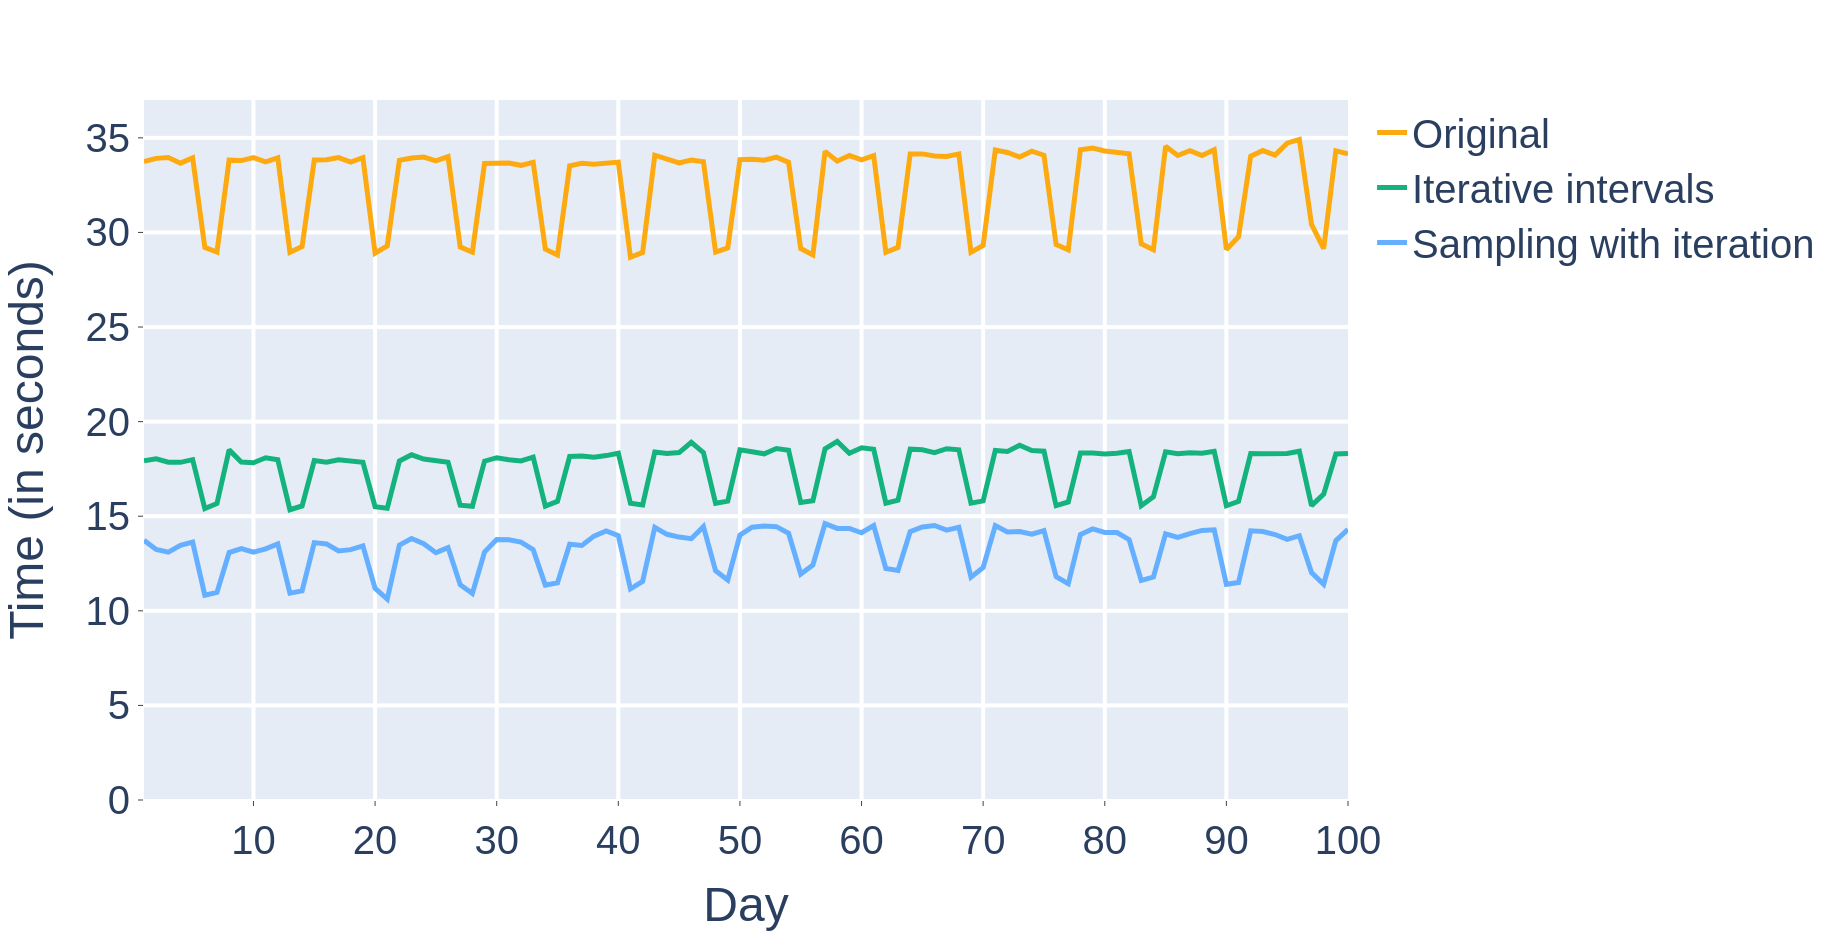
\includegraphics[width=\linewidth]{4 - Sampling/fig/sampling_with_iteration/swi_vs_rest_infector.png}
    \caption{Comparison of the infector runtimes between the different approaches.  Simulations run on 11M population for 100 days without holidays using 1 thread (configurations in Appendix \ref{appendix:configurations}).}
    \label{fig:swi_vs_rest_infector}
\end{figure}

\begin{table}
    \centering
    \begin{tabular}{@{}lrr@{}}
        \toprule
        \textsc{All-to-All} & Infector & Total \\ \midrule
        original & 32.63 & 33.77 \\
        sampling-with-iteration & 13.23 & 14.49 \\ \hdashline[1pt/1pt]
        speedup & 2.47 & 2.33 \\ \bottomrule
    \end{tabular}
    \caption{Comparison of the average daily runtimes between the original and \textsc{Sampling-with-iteration} approach. Simulations run on 11M population for 100 days without holidays using 1 thread (configurations in Appendix \ref{appendix:configurations}).}
    \label{tab:swi_vs_standard_runtimes}
\end{table}

\begin{figure}
    \centering
    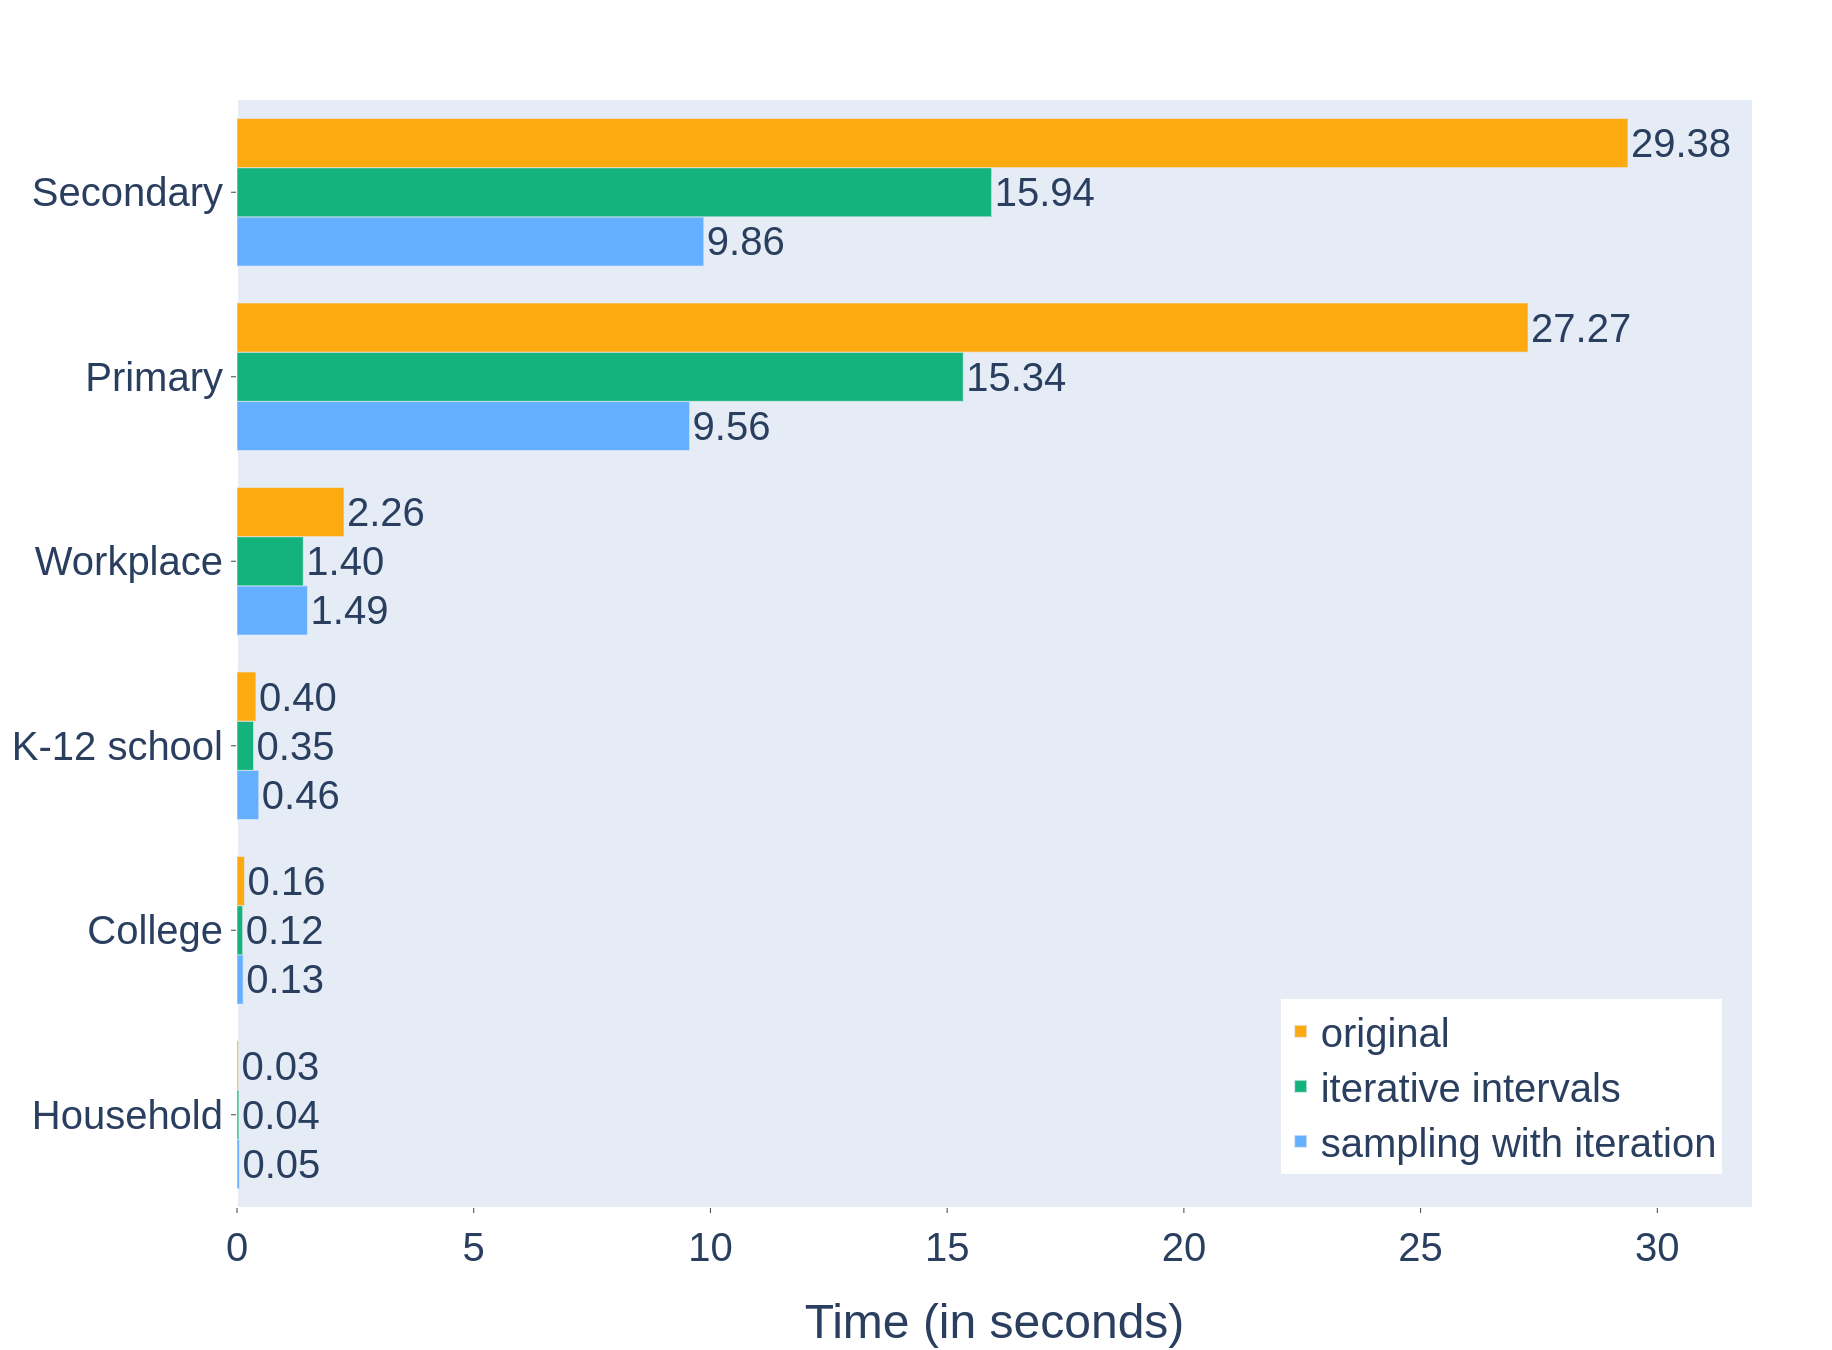
\includegraphics[width=\linewidth]{4 - Sampling/fig/sampling_with_iteration/swi_vs_rest_type_totals.png}
    \caption{Comparison of the total infector runtimes (in seconds) per pool type on a day in which its pools are active. Simulations run on 11M population for 100 days without holidays using 1 thread (configurations in Appendix \ref{appendix:configurations}).}
    \label{fig:swi_vs_rest_type_totals}
\end{figure}

\begin{figure}
    \centering
    \begin{subfigure}{.8\linewidth}
        \centering
        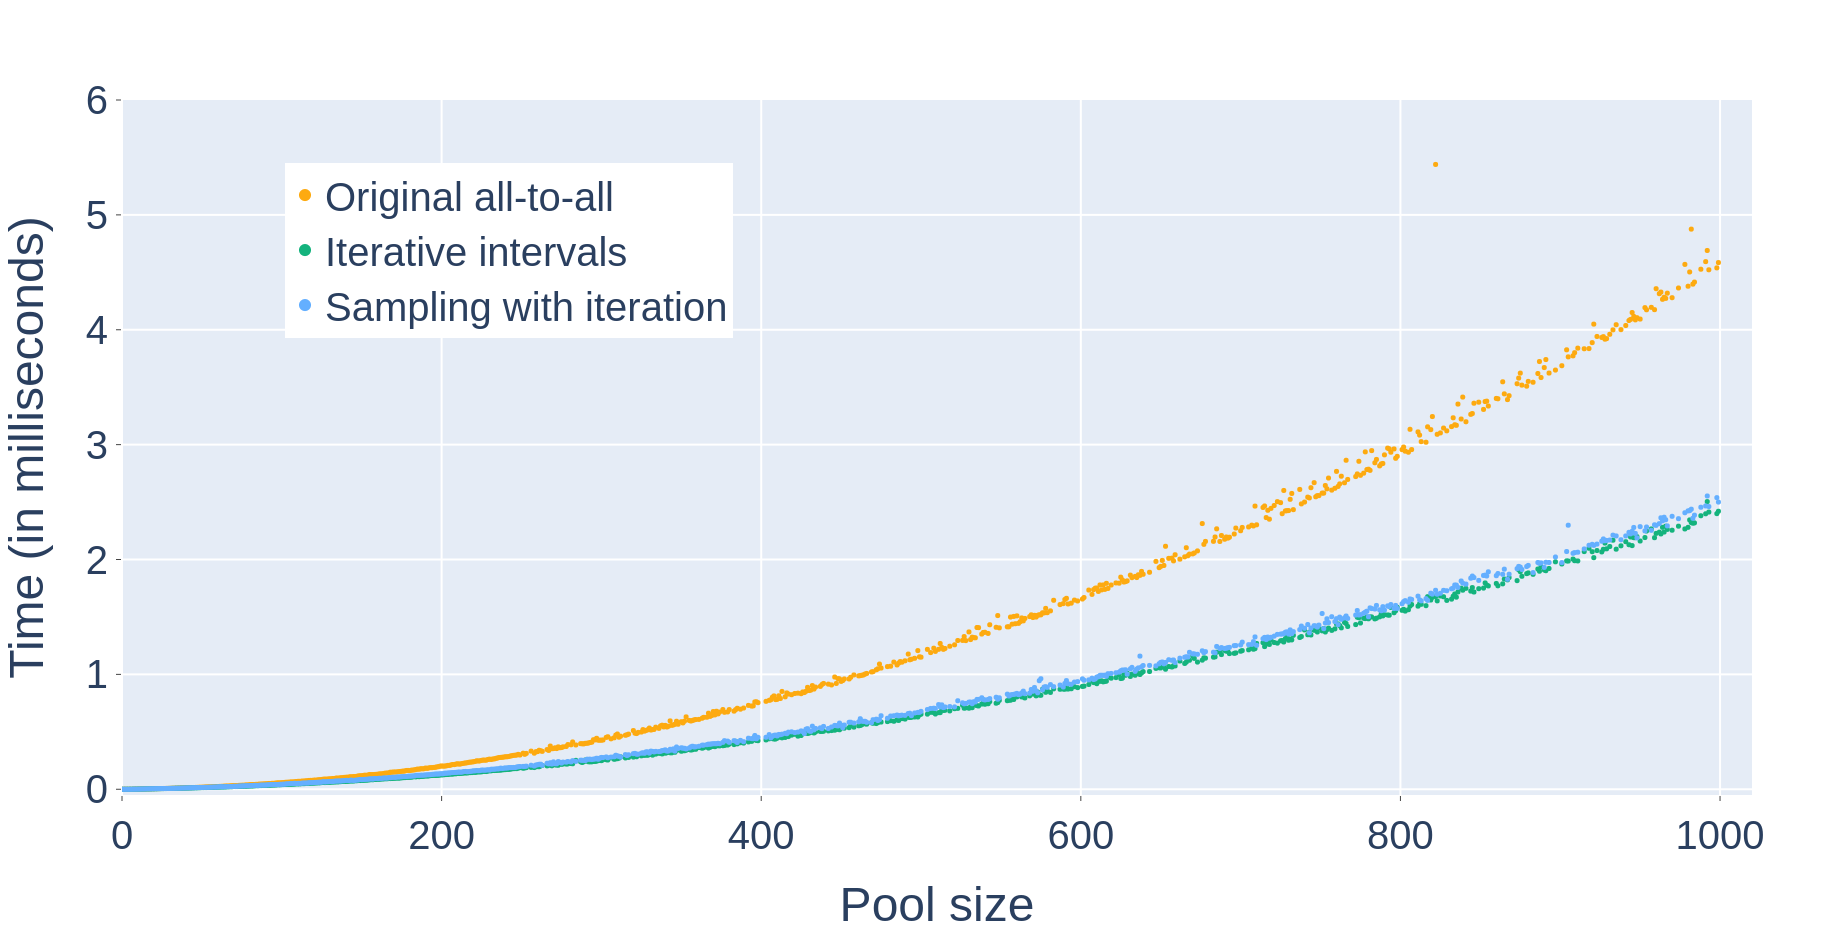
\includegraphics[width=\textwidth]{4 - Sampling/fig/sampling_with_iteration/times_avg_swi_pType_workplace_full.png}
        \caption{Workplace}
        \label{fig:times_avg_swi_pType_workplace_full}
    \end{subfigure}
    \begin{subfigure}{.8\linewidth}
        \centering
        \includegraphics[width=\textwidth]{4 - Sampling/fig/sampling_with_iteration/times_avg_swi_ptype_primary_full.png}
        \caption{Primary community}
        \label{fig:times_avg_swi_pType_primary_full}
    \end{subfigure}
    \begin{subfigure}{.8\linewidth}
        \centering
        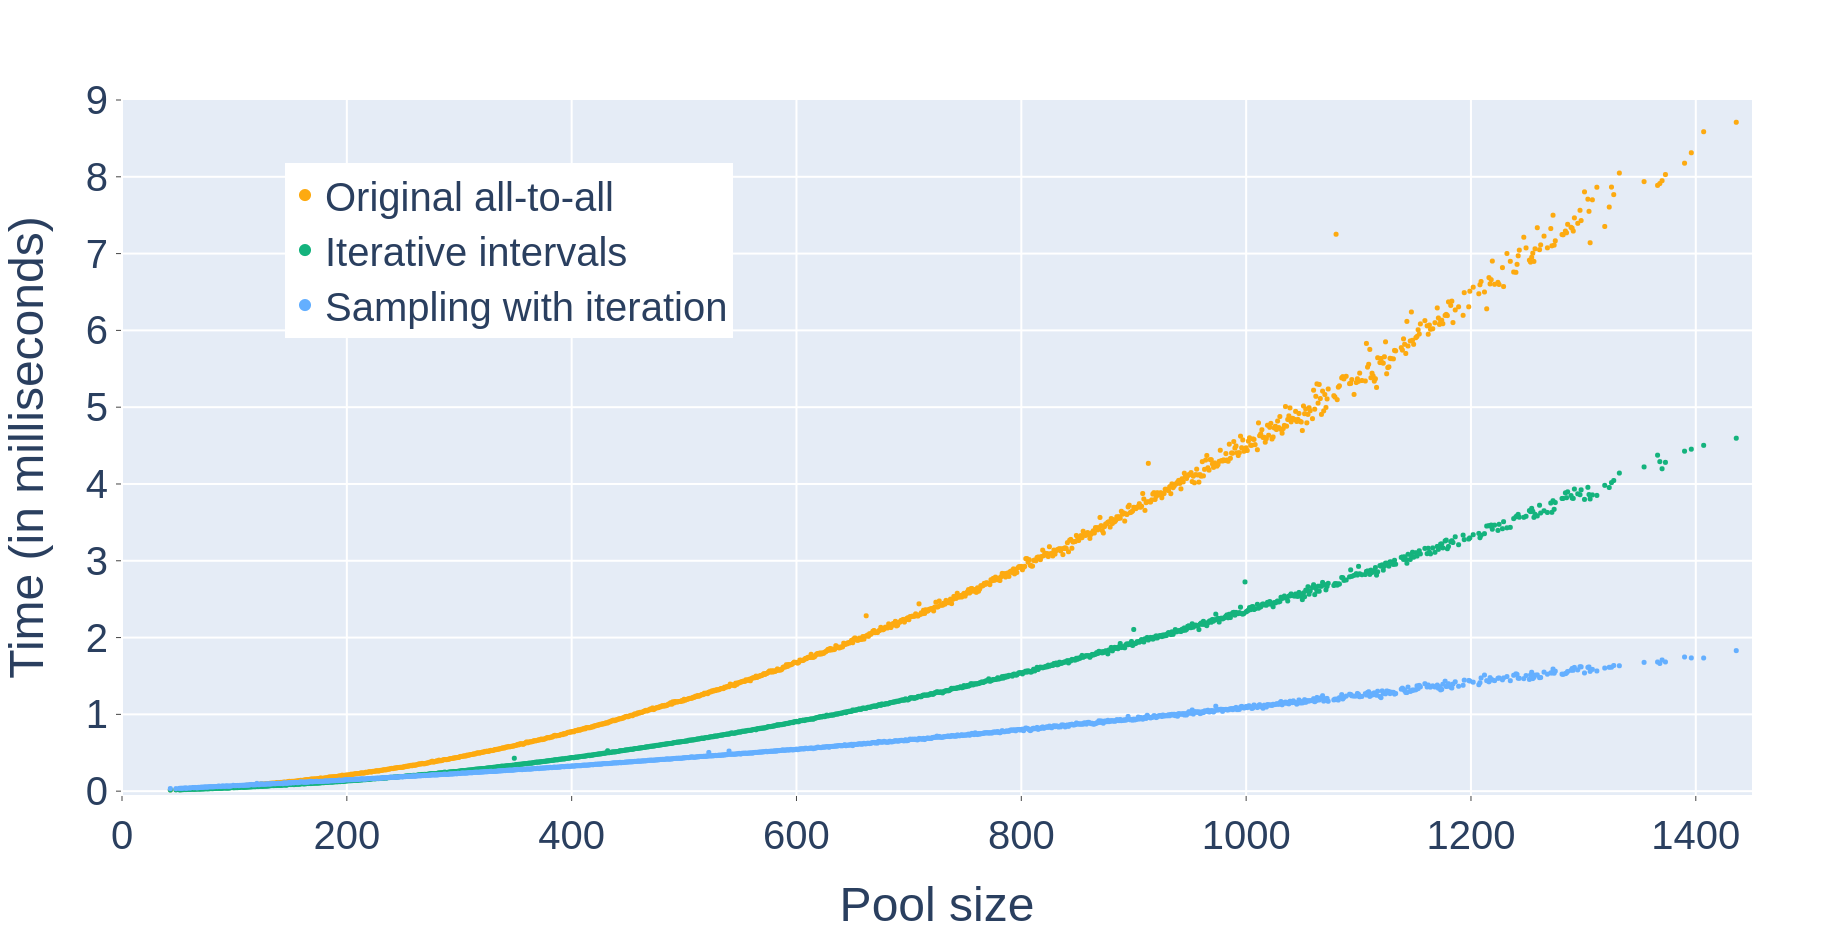
\includegraphics[width=\textwidth]{4 - Sampling/fig/sampling_with_iteration/times_avg_swi_pType_secondary_full.png}
        \caption{Secondary community}
        \label{fig:times_avg_swi_pType_secondary_full}
    \end{subfigure}
    \caption{Average infector runtimes (in milliseconds) per pool size using different approaches. Simulations run on 11M population for 100 days without holidays using 1 thread (configurations in Appendix \ref{appendix:configurations}).}
    \label{fig:times_avg_swi_pType_full}
\end{figure}

\begin{figure}
    \centering
    \begin{subfigure}{.8\linewidth}
        \centering
        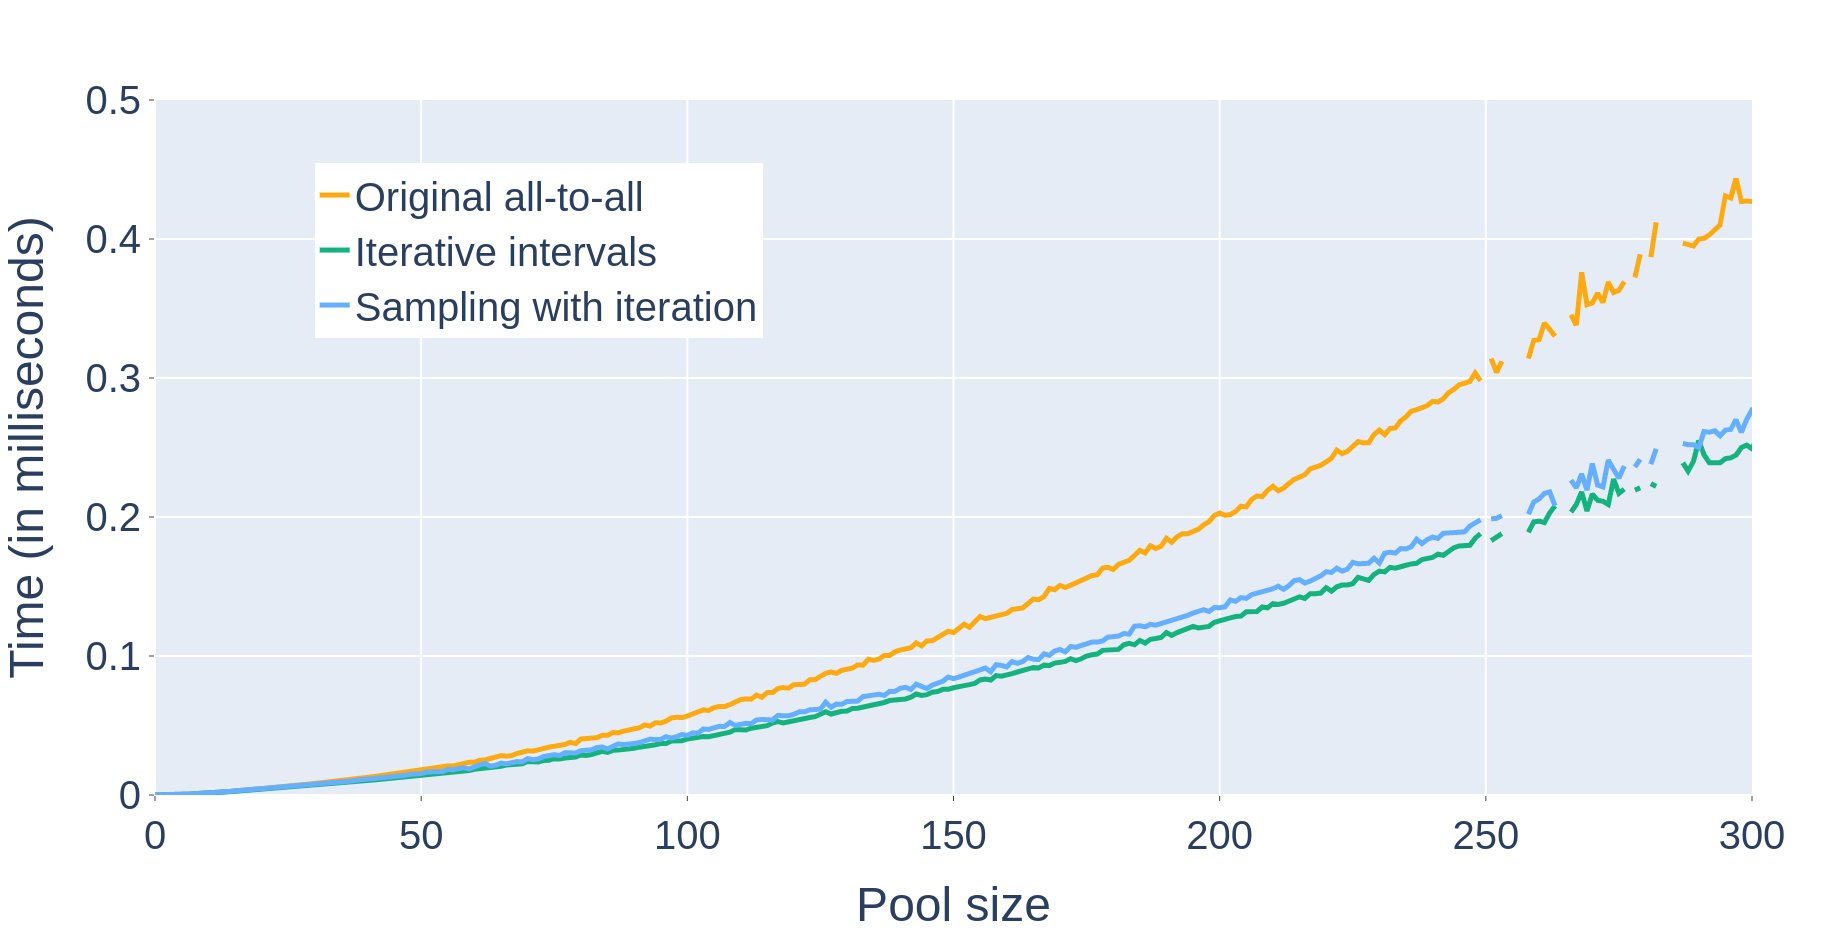
\includegraphics[width=\textwidth]{4 - Sampling/fig/sampling_with_iteration/times_avg_swi_pType_workplace.png}
        \caption{Workplace pool sizes [0, 300]}
        \label{fig:times_avg_swi_pType_workplace}
    \end{subfigure}
    \begin{subfigure}{.8\linewidth}
        \centering
        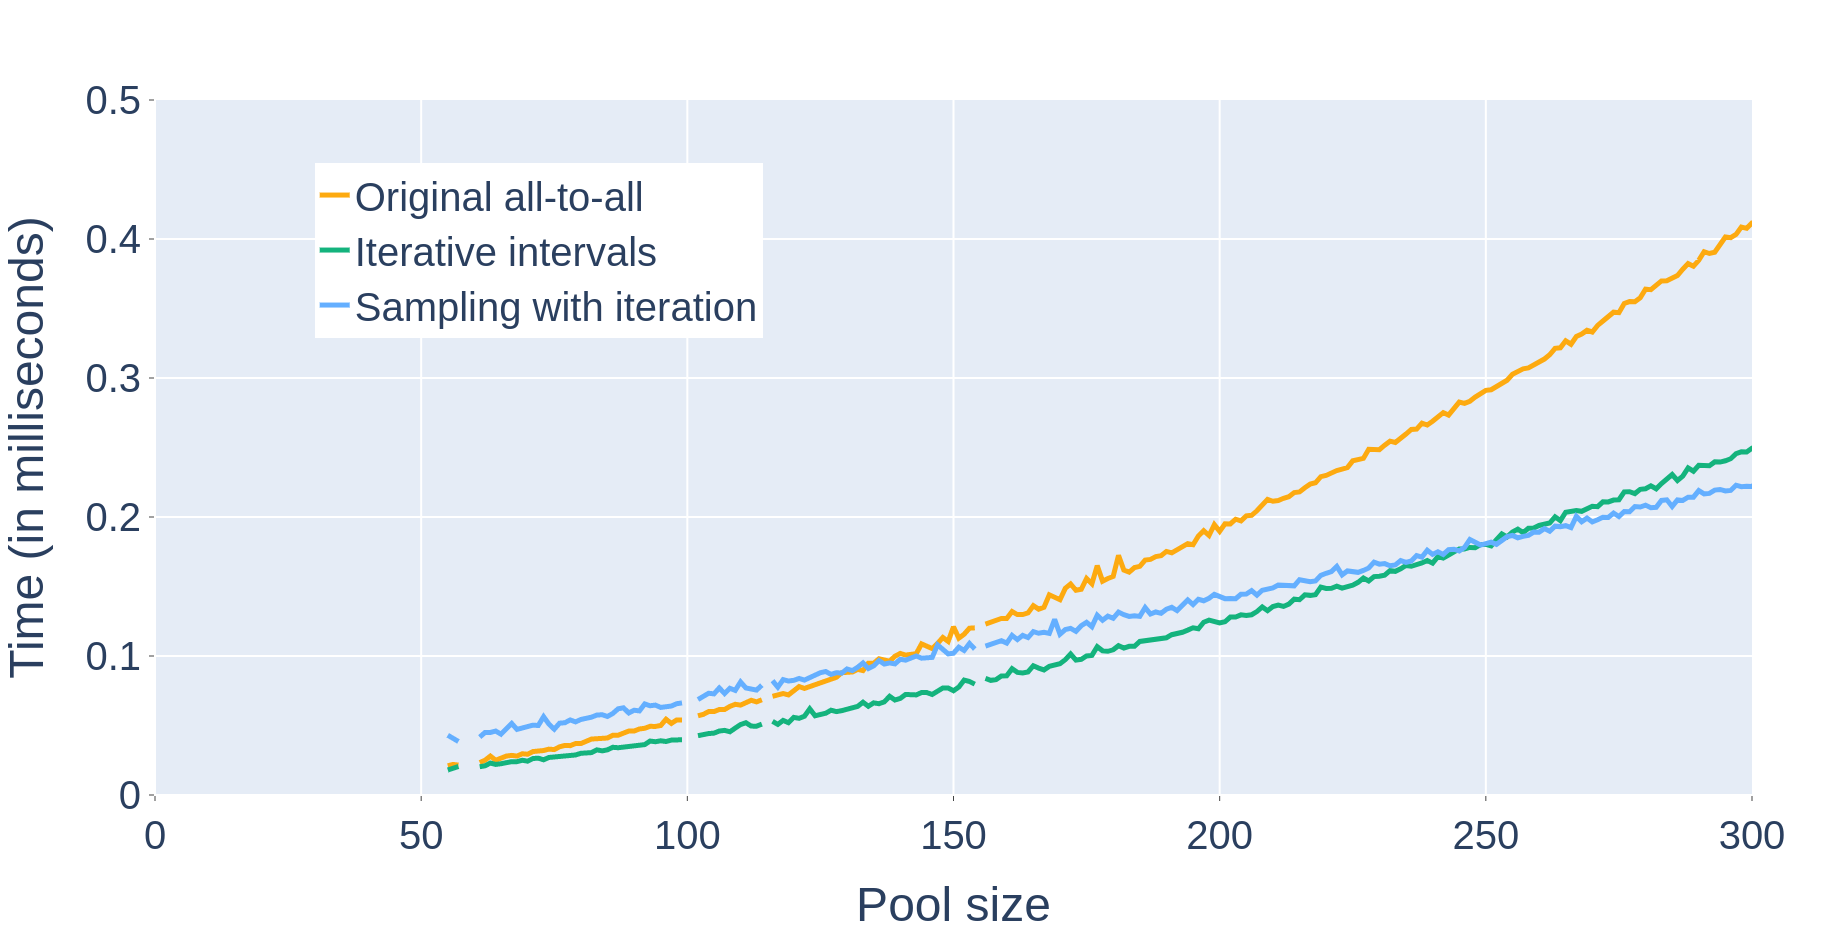
\includegraphics[width=\textwidth]{4 - Sampling/fig/sampling_with_iteration/times_avg_swi_pType_primary.png}
        \caption{Primary community pool sizes [0, 300]}
        \label{fig:times_avg_swi_pType_primary}
    \end{subfigure}
    \begin{subfigure}{.8\linewidth}
        \centering
        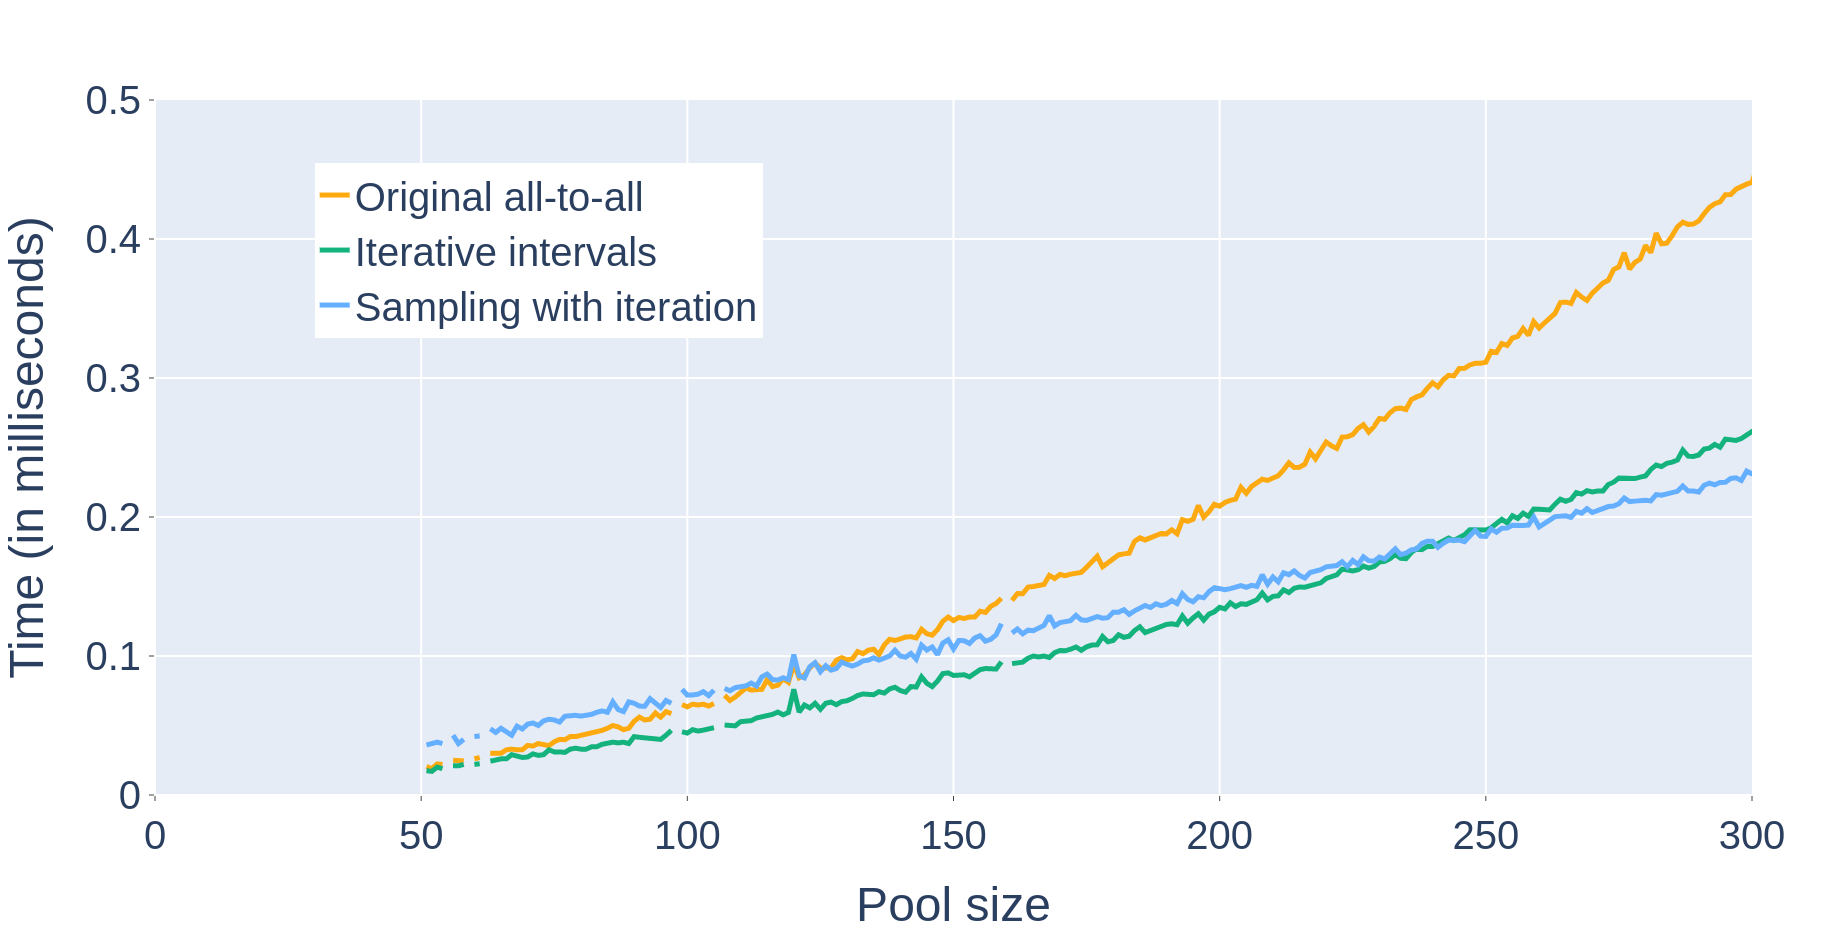
\includegraphics[width=\textwidth]{4 - Sampling/fig/sampling_with_iteration/times_avg_swi_pType_secondary.png}
        \caption{Secondary community pool sizes [0, 300]}
        \label{fig:times_avg_swi_pType_secondary}
    \end{subfigure}
    \caption{Average infector runtimes per pool size using different approaches. Simulations run on 11M population for 100 days without holidays using 1 thread (configurations in Appendix \ref{appendix:configurations}).}
\end{figure}
\begin{figure}\ContinuedFloat
    \centering
    \begin{subfigure}{.8\linewidth}
        \centering
        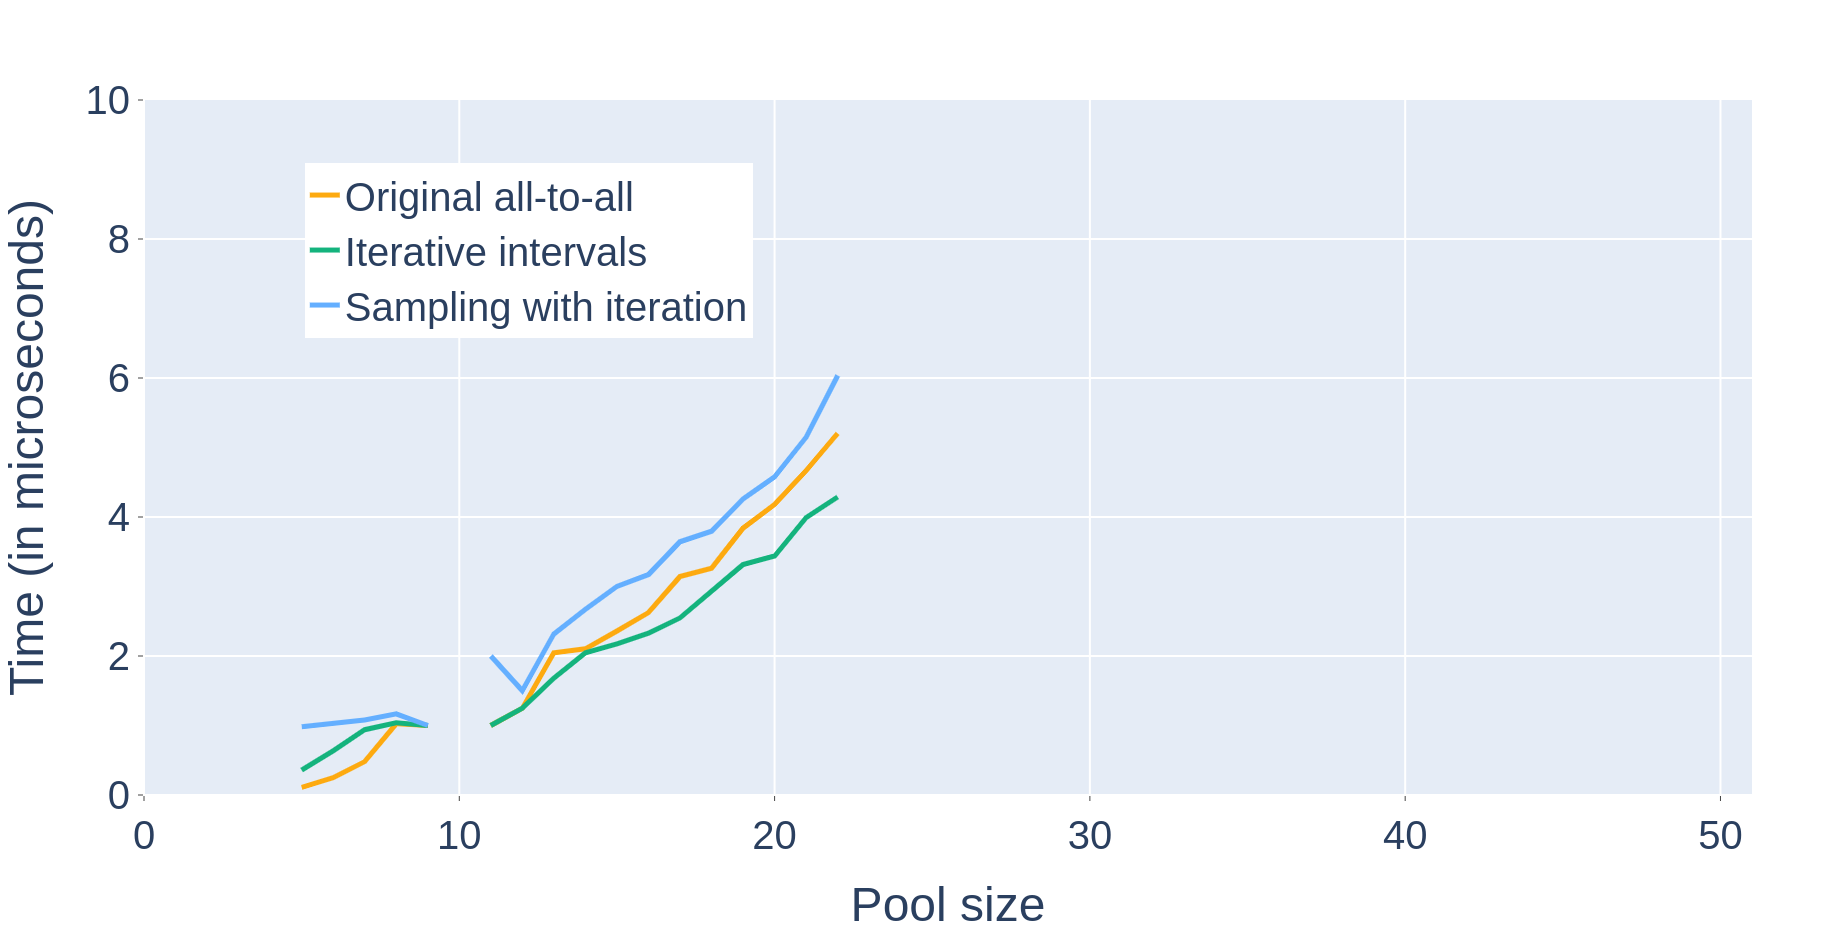
\includegraphics[width=\textwidth]{4 - Sampling/fig/sampling_with_iteration/times_avg_swi_pType_k12school.png}
        \caption{K-12 school}
        \label{fig:times_avg_swi_pType_k12school}
    \end{subfigure}
    \begin{subfigure}{.8\linewidth}
        \centering
        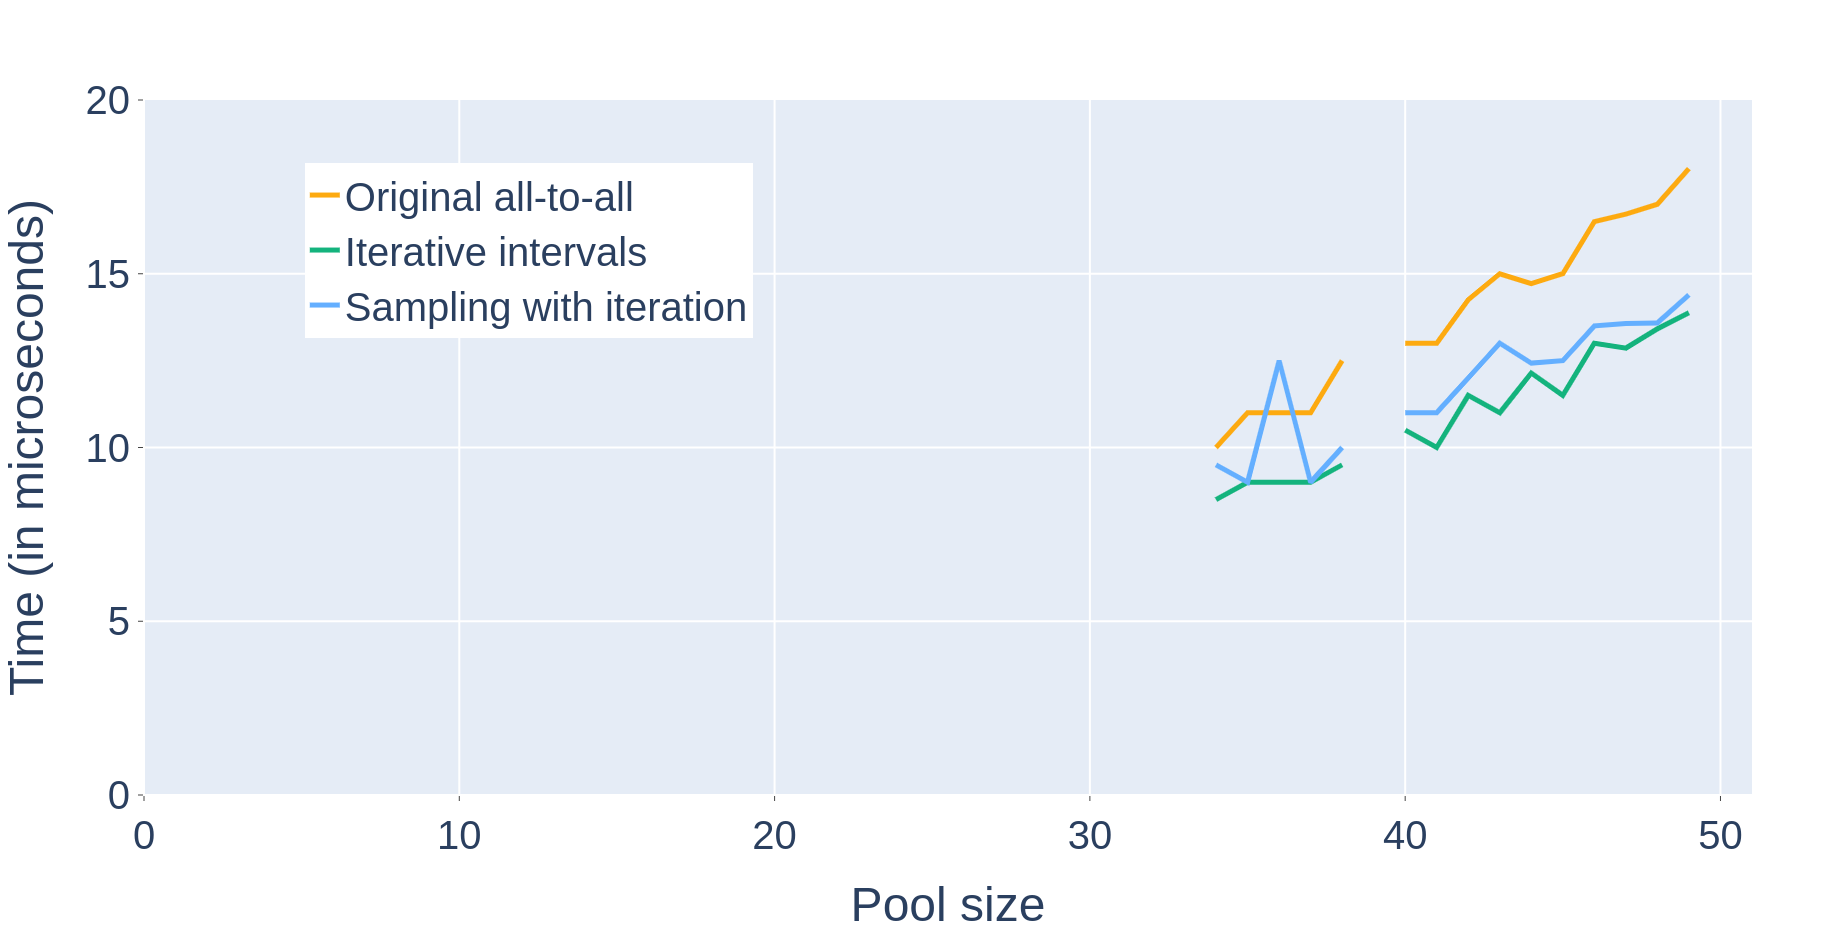
\includegraphics[width=\textwidth]{4 - Sampling/fig/sampling_with_iteration/times_avg_swi_pType_college.png}
        \caption{College}
        \label{fig:times_avg_swi_pType_college}
    \end{subfigure}
    \caption{Average infector runtimes per pool size using different approaches. Simulations run on 11M population for 100 days without holidays using 1 thread (configurations in Appendix \ref{appendix:configurations}).}
    \label{fig:times_avg_swi_pType}
\end{figure}

\subsection{Observations}
\label{subsec:observations_swi}
In the process of creating the \textsc{Sampling-with-iteration} approach as is, different implementations and techniques were examined in order to create the most optimal algorithm. These variations of the actual algorithm gave insights that are worth mentioning here.

\subsubsection{Pool size threshold}
Because we want to achieve the best runtimes, we want to minimise the parts where our \textsc{Sampling-with-iteration} acts slower than the rest. As we learned from Figure \ref{fig:times_avg_swi_pType}, the original algorithm is faster for the pools with maximum 150 people. Therefore, we adjusted Algorithm \ref{alg:sampling_with_iteration} so that pools with 150 individuals or less make use of the original \textsc{All-to-All} algorithm instead of only the household pools. After testing this theory, the results did not improve compared to only separating the household pools from the rest and were even worse most of the times. The most plausible explanation for this is \textit{branch prediction}, which is an optimisation technique for the processor \cite{branch_prediction}. When there are multiple branches in a program, such as in an if-then-else-structure, the processor tries to guess which branch it will need to execute and commences to execute the instructions of a particular branch, which is called \textit{speculative execution} \cite{speculative_execution}. The execution then becomes faster on a low-level, because it does not have to wait for the result of the condition, which is slow, to follow the conditional jump to the instructions. However, if the speculations turn out to be incorrect, the already performed computations are discarded and the right instructions get executed and causes the execution to slow down by a couple of clock cycles. The more mispredictions, the slower the execution of course. 
\\\\
Our \textsc{Sampling-with-iteration} algorithm only uses the original method on household pools. Algorithm \ref{alg:infector} showed us how the infector is called for all pools, which iterates over the pools of a particular type before continuing to the pools of the next type. Thus when the processor predicts the branch, it is only wrong when the previous pool was a household pool and the next one is a different type or vice versa. Therefore, the branch prediction technique works very well with how we implemented our algorithm. When we changed the if-test to check for pools with less than 150 people, it caused a lot of mispredictions because subsequent pools in the iteration have different sizes. The household, K-12 school and college pools never contain more than 150 individuals, thus they are not affected by this. However, the workplace and both community pools can have very large sizes, which results in a a lot of mispredictions. Therefore, this overhead is the cause that implementing such a threshold based on the pool size makes the execution more time-consuming. A solution to this is to sort the pools based on their sizes when initialising the simulation, but this has not been examined because it would most likely not significantly increase performance.

\subsubsection{Sorting at initialisation}
Every non-household pool gets sorted in age intervals every time their contacts and transmissions need to be calculated. Since we use a population in which the individuals always remain the same age and the pools contain the same people, this sorting procedure can easily be implemented at the start of the simulation in the initialisation. This has been tested, but did not result in faster execution times. Also, the simulation can also switch between \textsc{All-to-All} and \textsc{Inf-to-Sus} from one day to another based on what needs to be calculated. For these reasons, it is therefore best to use the \textsc{Sampling-with-iteration} as originally described, which gives our method also the possibility to work with dynamic populations and pools.

\subsubsection{One sample size}
This new approach, for which the pseudo code is given in Algorithm \ref{alg:sampling_with_iteration}, shows that a sample size gets calculated for every member $P_{1}$ when iterating over $interval_{1}$. This means that the binomial distribution that uses a random number generator is used for every $P_{1}$, which is a rather costly operation compared to, for example, a simple if-test in terms of execution time. Computing the sample size only once for an entire pair of intervals would thus reduce these costs. After examining this implementation, it could be concluded that it indeed produced faster results and that it passed the built-in testing tool. However, the reversed contact rates did not match the original ones as can be seen in Figure \ref{fig:swi_1sample_vs_standard_reversed_cr}. The K-12 school, college, and workplace reversed contact vectors were very similar to the original ones because they do not contain that many different non-empty intervals. On the other hand, the primary and secondary community pools their reversed contact rates were reasonably different than the original rates. The only difference regarding our actual \textsc{Sampling-with-iteration} is that there is less randomness involved due to computing only one sample size. The explanation for these results is the law of large numbers \cite{law_large_numbers}, which states that the outcome is closer to the expected outcome the more trials are performed. Therefore, determining only one sample size has a very big impact on the contacts between two intervals. Normally, a sample size gets calculated multiple times which thus evens out the odd results. The reason that this passed the built-in test, is because in the end, the law of large numbers is applicable because a lot of sample sizes have been calculated. The reversed contact vectors are thus essential in testing our different approaches.

\begin{figure}
    \centering
    \begin{subfigure}{.8\linewidth}
        \centering
        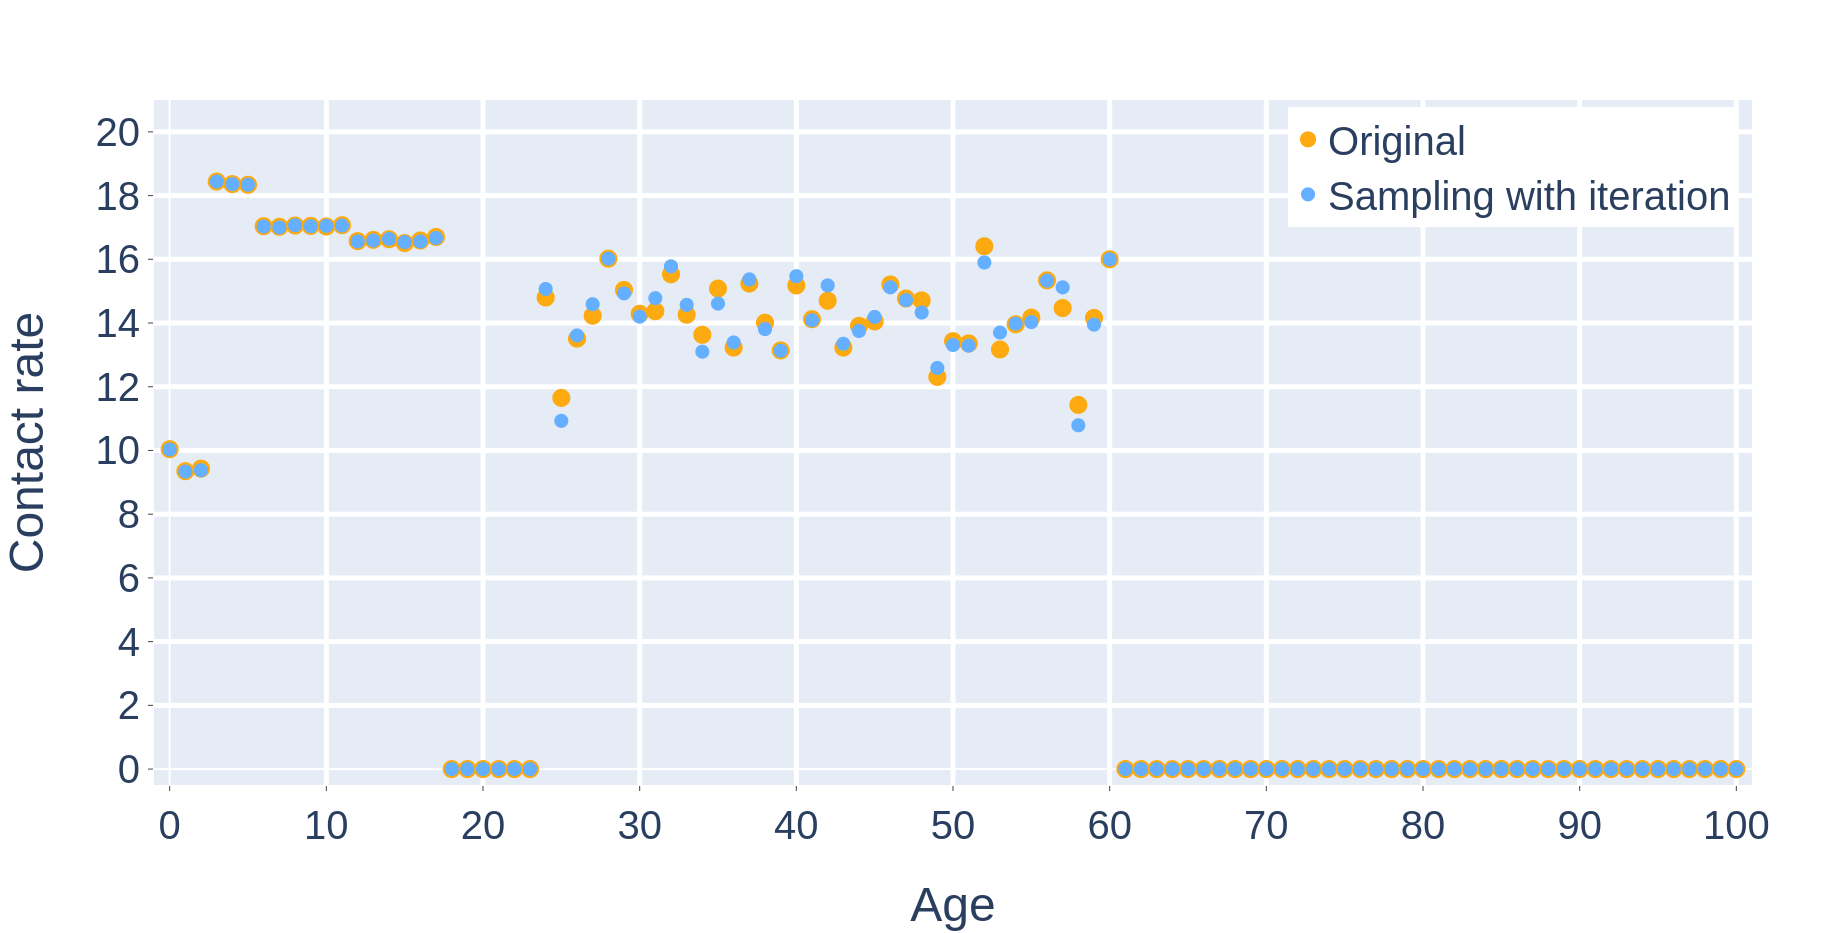
\includegraphics[width=\textwidth]{4 - Sampling/fig/sampling_with_iteration/swi_1sample_vs_standard_reverse_cr_k12school.png}
        \caption{K-12 school}
        \label{fig:swi_1sample_vs_standard_reversed_cr_k12school}
    \end{subfigure}
    \begin{subfigure}{.8\linewidth}
        \centering
        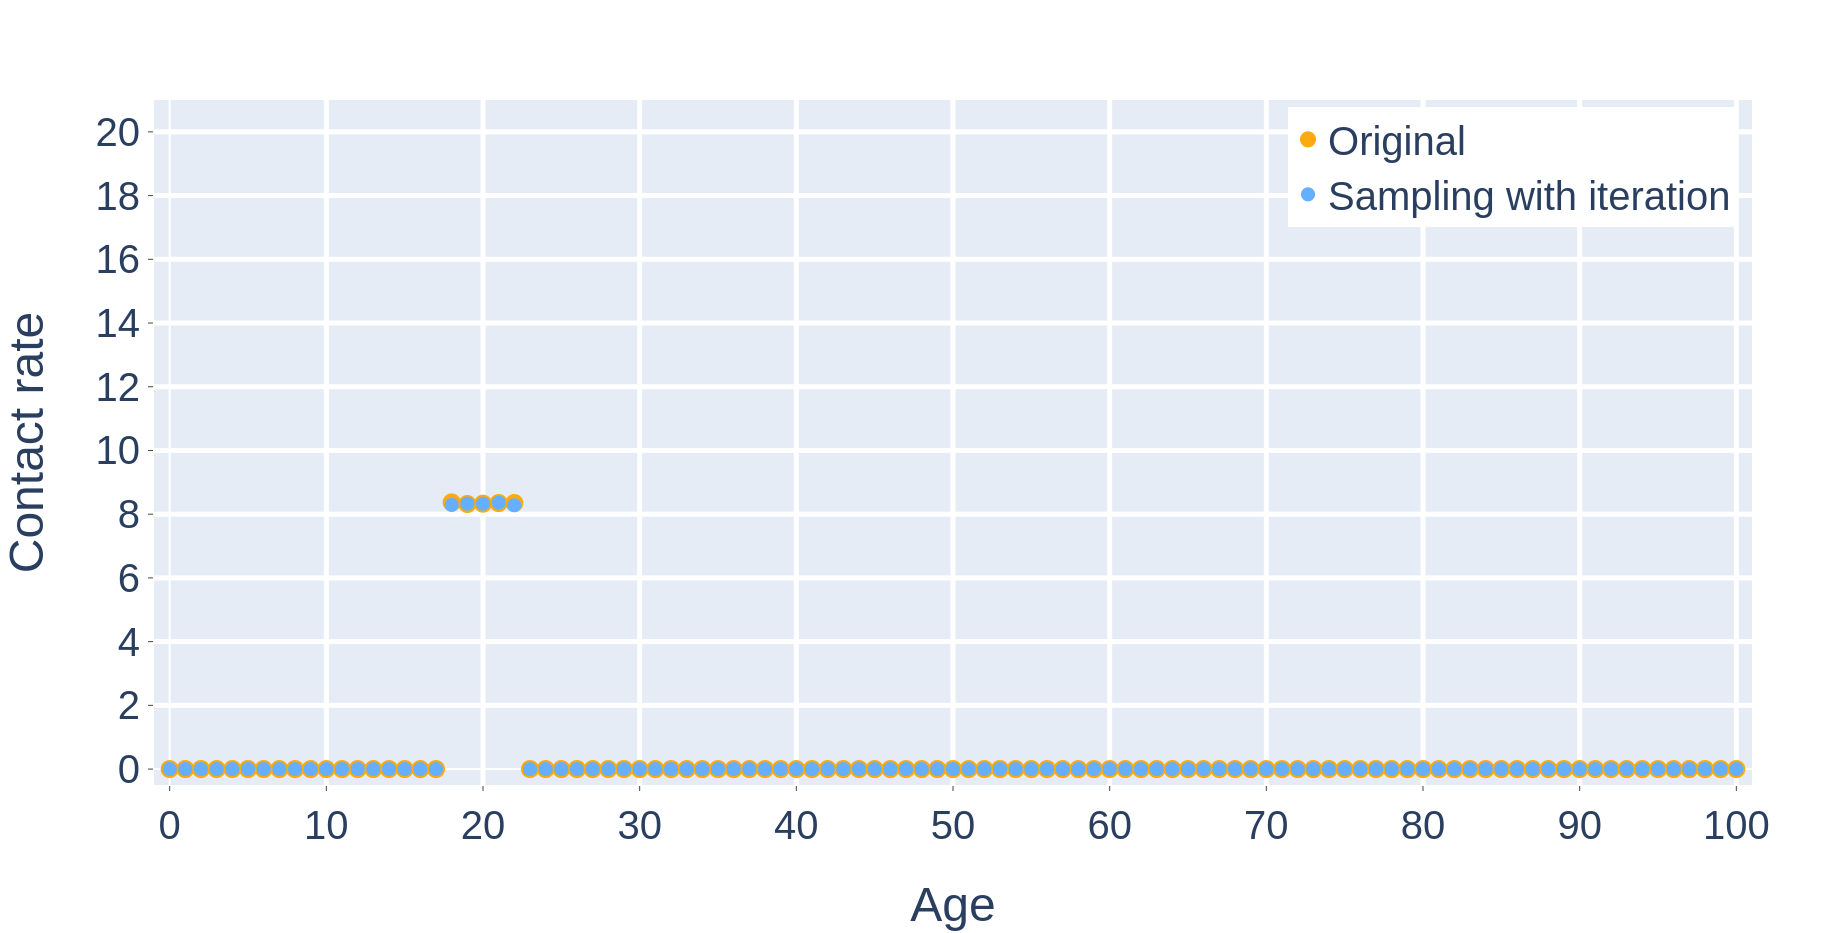
\includegraphics[width=\textwidth]{4 - Sampling/fig/sampling_with_iteration/swi_1sample_vs_standard_reverse_cr_college.png}
        \caption{College}
        \label{fig:swi_1sample_vs_standard_reversed_cr_college}
    \end{subfigure}
    \begin{subfigure}{.8\linewidth}
        \centering
        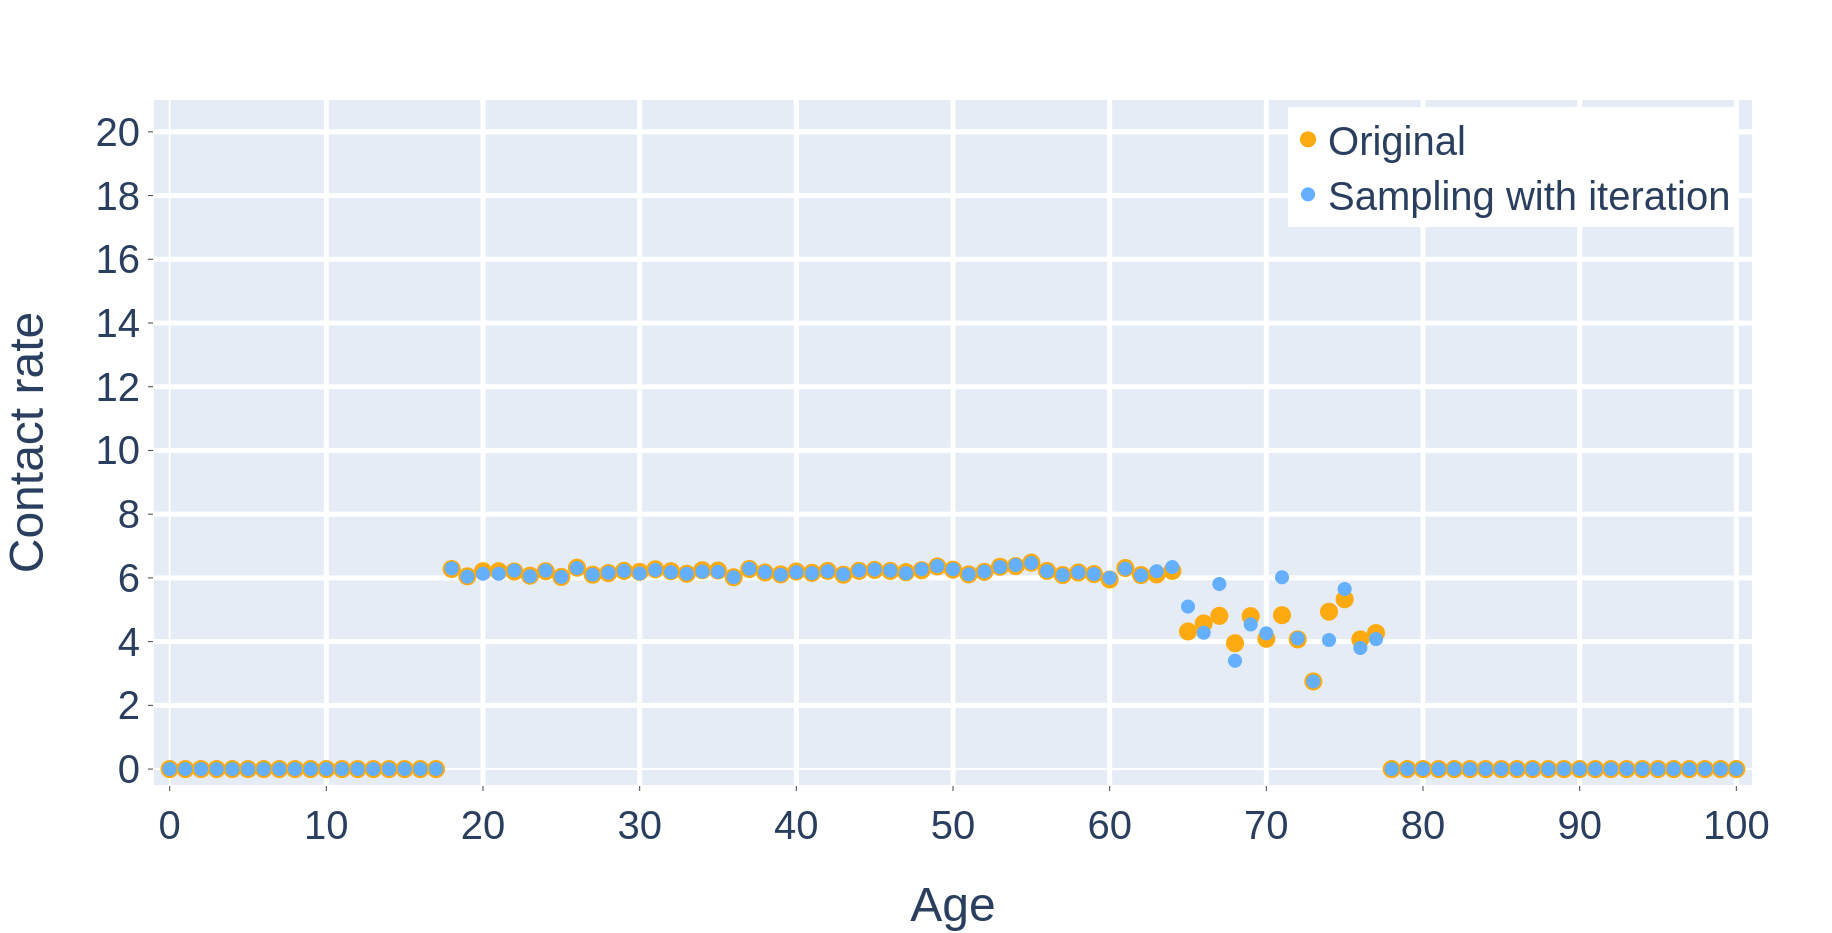
\includegraphics[width=\textwidth]{4 - Sampling/fig/sampling_with_iteration/swi_1sample_vs_standard_reverse_cr_workplace.png}
        \caption{Workplace}
        \label{fig:swi_1sample_vs_standard_reversed_cr_workplace}
    \end{subfigure}
    \caption{The reversed contact rates of \textsc{Sampling-with-iteration} using one sample size per interval compared to the original \textsc{All-to-All} reversed contact rates.}
\end{figure}
\begin{figure}\ContinuedFloat
    \centering
    \begin{subfigure}{.8\linewidth}
        \centering
        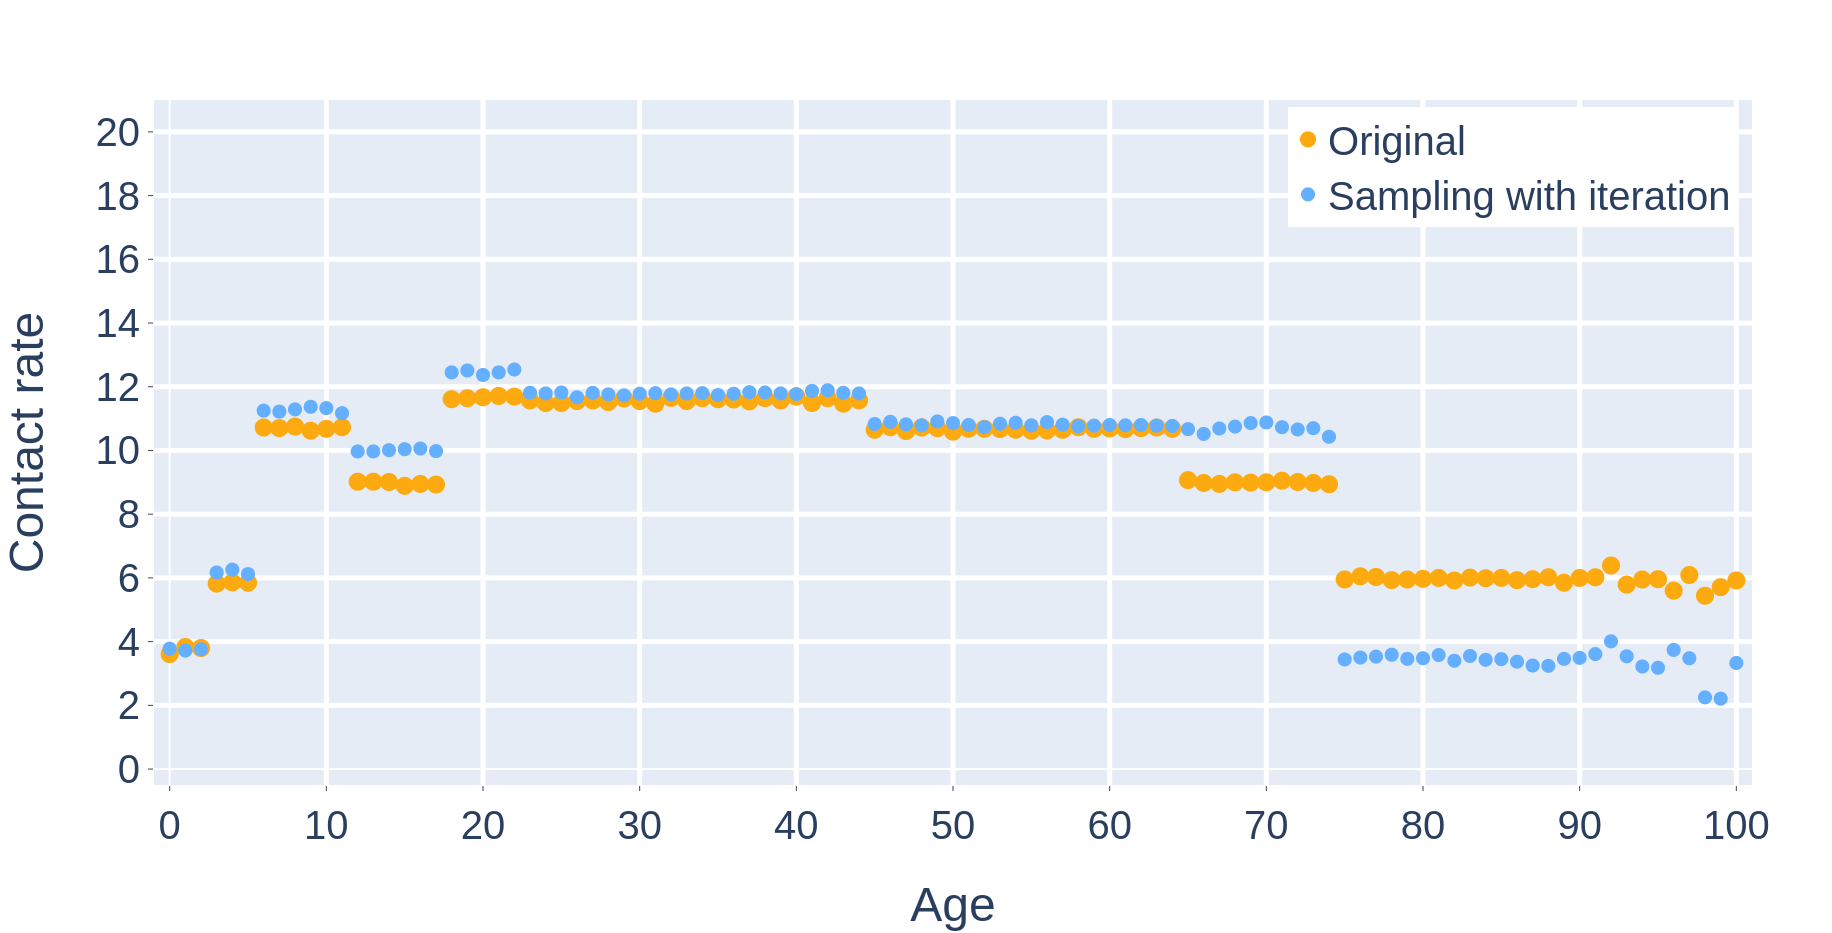
\includegraphics[width=\textwidth]{4 - Sampling/fig/sampling_with_iteration/swi_1sample_vs_standard_reverse_cr_primary.png}
        \caption{Primary community}
        \label{fig:swi_1sample_vs_standard_reversed_cr_primary}
    \end{subfigure}
    \begin{subfigure}{.8\linewidth}
        \centering
        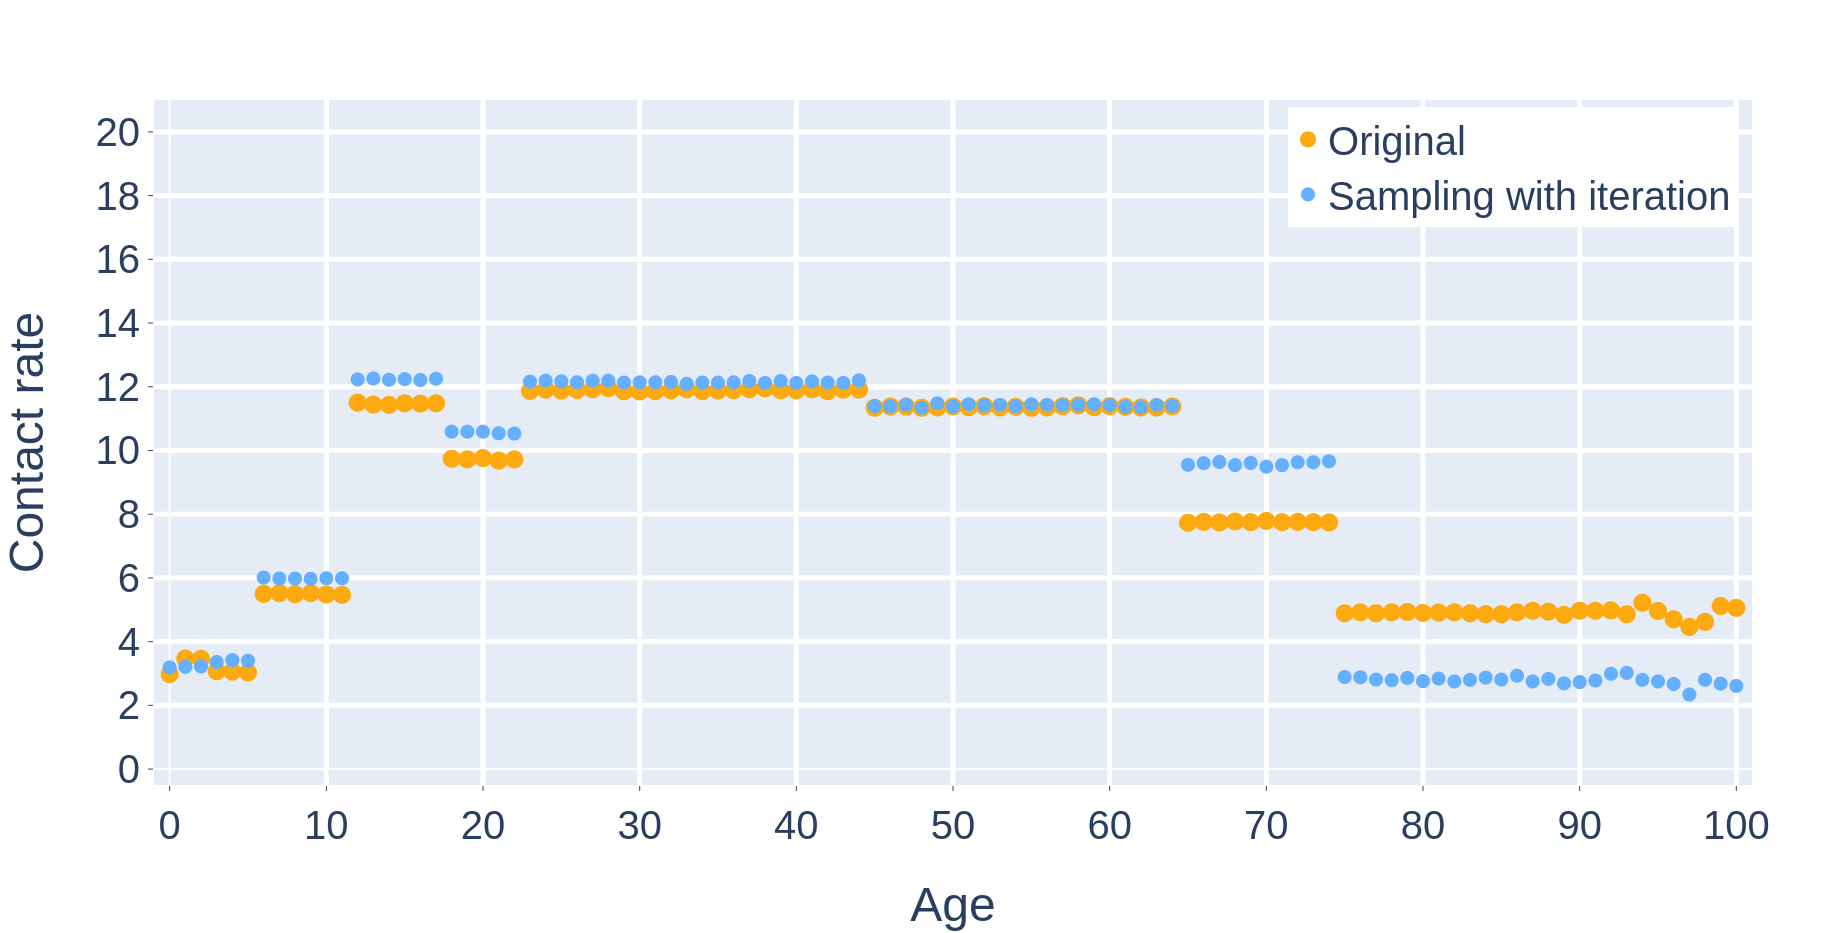
\includegraphics[width=\textwidth]{4 - Sampling/fig/sampling_with_iteration/swi_1sample_vs_standard_reverse_cr_secondary.png}
        \caption{Secondary community}
        \label{fig:swi_1sample_vs_standard_reversed_cr_secondary}
    \end{subfigure}
    \caption{The reversed contact rates of \textsc{Sampling-with-iteration} using one sample size per interval compared to the original \textsc{All-to-All} reversed contact rates.}
    \label{fig:swi_1sample_vs_standard_reversed_cr}
\end{figure}

\subsubsection{Storing drawn individuals}
When a sample size is determined for a member $P_{1}$, the contacts get randomly selected one by one. Once a random contact has been chosen, the algorithm needs to check that this person did not already have contact in the same iteration with $P_{1}$. The persons that $P_{1}$ already had contact with in the same iteration are stored in a \textit{std::vector} \cite{vector} by their indexes. For every $P_{1}$ a new, empty vector gets created with a size that is the same as the number of people in the other interval. Searching if an element exists in such a vector has a linear time complexity in function of the size of the vector. Our algorithm already optimises this by storing the indexes subsequently, starting at the first element. Checking if an index already appears in the vector is then performed by only checking the elements of the vector that are not empty, which reduced the total infector runtime by several seconds.  Another option that has been tested is by replacing the \textit{std::vector} with a \textit{std::unordered\_set} \cite{unordered_set}, which is a hash map that has a constant time complexity for lookups. The daily total infector runtime was, however, a little bit slower than the current approach. The reason for this is that the sample sizes are very small and are rarely higher than five, which only happens if the interval is very large. Although the hash map has a constant lookup time, it has more overhead than the regular vector. Since most of the lookups are executed when there are zero or one indexes stored, the overhead from \textit{std::unordered\_set} causes it to be slower.
\\\\
The creation of a vector also comes with some overhead, hence we tried to minimize this overhead by creating the vector only once per pair of intervals. After every $P_{1}$ this vector needs to be emptied for the next one, which also has some overhead. Examining these results indicated that emptying the vector costs more time than deleting and creating a new vector. Another option to reduce the time is by creating a smaller vector, since only a small part of it gets actually used. This is not entirely true, because it is possible for almost an entire interval to be absent due to illness, which would cause the vector to fill up if those absent members are drawn. Choosing for example halve the original size to create the vector and only increasing its size when necessary is probably also not an option, because this would cause overhead due to extra tests to handle the vector.

\section{Full sampling}
\label{sec:full_sampling}
We learned from \textsc{Sampling-with-iteration} that the algorithm did not improve the infector runtime for workplace pools, because most of the contact calculations were between people in the same age interval. In order to improve this, the algorithm needs an update on how to compute these same interval calculations and, since sampling has such good results, we want to use sampling for these computations. As we already discussed in the previous section, there is no straightforward way to implement this and still produce correct results. Examples \ref{ex:fs_wrong1} and \ref{ex:fs_wrong2} present ideas that have been considered while also explaining why they would not work.
\begin{example}
\label{ex:fs_wrong1}
Consider an age interval with $N$ members for which we need to calculate the contacts between the members of said interval. We could iterate over the members, starting from member $1$ up to $N$. For every member $i$, we calculate the sample size based on $N-i$ members and only randomly select contacts between members $i+1$ till $N$. There are two reasons that this approach would not work:
\begin{enumerate}
    \item Starting at member $1$, the rest of the members are all considered as a possible contact. If we then move on to member $2$, member $1$ is not considered as a contact anymore and will thus have much less contacts than member $N$ and result in incorrect results.
    \item We have learned that sampling is ineffective when the intervals are small because of the overhead that comes with it. Because we gradually decrease our `interval' from which we draw contacts, this will cause our approach to perform worse than just comparing everyone with each other.
\end{enumerate}
\end{example}
\begin{example}
\label{ex:fs_wrong2}
Consider again the age interval with $N$ members for which we want to calculate the contacts between its members. To prevent our interval to decrease in size, we now iterate over our members and keep the interval size the same. Every member $i$ will thus have a sample size based on $N$ and will select contacts from all $N$ members in the interval. This results in everyone being considered the same amount of times. If we then look at the pair of individuals that have been considered, we see that the contact between member $i$ and member $j$ has been considered twice, namely once when calculating contacts for member $i$ and once when calculating contacts for member $j$. Thus, the algorithm would have calculated twice the amount of contacts that should have been calculated. In order solve this, we simply divide the contacts by two. Unfortunately, there are also various reasons that this would not work:
\begin{enumerate}
    \item Calculating twice the amount of contacts would of course significantly decrease the speedup.
    \item When we delete half of the contacts, how do we decide which ones that need to be nullified?
    \item If we already calculated contacts for $i$, among which $j$, what needs to be done if we draw $i$ when calculating contacts for $j$?
    \item Implementing this, would require us to keep track of all the contacts, so that we can delete half of them at the end. Storing this and then selecting half of the contacts would create significant overhead and maybe even result in even worse runtimes.
\end{enumerate}
\end{example}

A solution to our problem should therefore lie somewhere in the middle between these two examples. We do not want to calculate redundant contacts, because this would increase the execution time. On the other hand, only calculating the necessary contacts might be impossible to achieve with sampling. Therefore, the solution that we present might calculate the same contacts twice, but it lets us iterate over the entire interval without needing to select the `real' contacts at the end. This is achieved by calculating the contact probability in another way, so that it can be used in the binomial distribution when computing sample sizes while always considering the entire interval as possible contacts. The method for calculating the contact probability in Algorithm \ref{alg:contact_probability} is slightly adjusted by replacing line 8 with the following:
$$p = \frac{2-\sqrt{4-4\frac{r}{n-1}}}{2}\text{, with interval size }n\text{ and contact rate }r$$
The reasoning behind this and the proof that it should work are presented in Appendix \ref{appendix:sampling_same_interval}. Let it be noted that this contact probability is only used for the contact calculations in the same interval, thus comparing two different intervals still uses the original method. Because this algorithm uses sampling in all occasions, except for the household pools, it will be referred to from now on as the \textsc{Full-sampling} approach.

\subsection{Implementation}
\label{subsec:implementation_full_sampling}
Algorithm \ref{alg:full_sampling} shows the pseudo code of \textsc{Full-sampling}, where the only difference with the \textsc{Sampling-with-iteration} approach is the case when $interval_{1}$ is equal to $interval_{2}$. When our model now calculates the contacts between people in the same age interval, it iterates over the interval's members and calculates a sample size based on the number of people in the interval and the adjusted contact probability. It then operates the same as regular sampling by keeping track of who has already been drawn and randomly selects people in the entire interval. An additional issue is solved by adding $P_{1}$ as an `already drawn' member, to prevent someone from having contact with themselves. We also discussed the problem of people having contact twice with each other in the same pool on the same day. When this happens, both contacts are handled and registered as valid independent events. If a transmission occurs, it will only happen the first time because the second time none of the members is susceptible, which thus does not interfere with the normal simulation flow.

\begin{algorithm}
\caption{Pseudo code of the \textsc{All-to-All} \textsc{Full-sampling} infector.}
\label{alg:full_sampling}
\begin{algorithmic}[1]
    \Require{$P_{1} \dots P_{N}$, $type$} \Comment{All members of the pool and type of pool}\;
    \Statex
    \If{$type = household$}
        \State original \textsc{All-to-All} \Comment{Algorithm \ref{alg:all-to-all}}
    \Else
        \State $S[\;] \gets$ \Call{sort\_intervals}{$P[\;], type$}\Comment{Algorithm \ref{alg:age_sorting}, returns interval sizes}
        \State $N_{intervals} \gets$ \Call{sizeof}{$S[\;]$} \Comment{Number of intervals}
        \Statex
        \For{$interval_{1} \gets 1$ to $N_{intervals}$} \Comment{Iterate intervals}
            \For{$interval_{2} \gets interval_{1}$ to $N_{intervals}$} \Comment{Iterate remaining intervals}
                \Statex
                \If{$interval_{1} = interval_{2}$}
                    \State $C_{prob} \gets$ \Call{special\_cprob}{$interval_{1}$} \Comment{Appendix \ref{appendix:sampling_same_interval}}
                    \Foreach{member $P_{1}$ in $interval_{1}$}
                        \If{$P_{1}$ not in pool}
                            \State continue to next $P_{1}$
                        \EndIf
                        \State $sample \gets$ \Call{binomial}{$S[interval_{1}], C_{prob}$} \Comment{Binomial distribution}
                        \If{$sample$ = 0}
                            \State continue to next $P_{1}$
                        \ElsIf{$sample$ = $S[interval_{2}]$}
                            \State iterate over $interval_{2}$ and register contact with everyone
                        \Else
                            \State $drawn\_members \gets [\;]$
                            \State add $P_{1}$ to $drawn\_members$
                            \State $draws_{all} \gets 1$ \Comment{Number of draws, already `drawn' $P_{1}$}
                            \State $draws_{good} \gets 0$ \Comment{Number of good draws}
                            \Statex
                            \While{$draws_{good} < sample$ AND $draws_{all} < S[interval_{1}]$}
                                \State $P_{2} \gets$ random member of $interval_{1}$
                                \If{$P_{2}$ in $drawn\_members$}
                                    \State draw next $P_{2}$
                                \EndIf
                                \State add $P_{2}$ to $drawn\_members[\;]$
                                \State $++draws_{all}$
                                \If{$P_{2}$ not in pool}
                                    \State draw next $P_{2}$
                                \EndIf
                                \State $++draws_{good}$
                                \State register contact
                                \If{$P_{1}$ or $P_{2}$ susceptible and other infectious}
                                    \State $T_{prob} \gets$ transmission probability
                                    \If{\Call{BernoulliTrial}{$T_{prob}$}}
                                        \State infect the susceptible one
                                    \EndIf
                                \EndIf
                            \EndWhile
                        \EndIf
                    \EndForeach
                \Else
                    \State regular sampling between two different intervals \Comment{Algorithm \ref{alg:sampling_with_iteration}}
                \EndIf
            \EndFor
        \EndFor
    \EndIf
\end{algorithmic}
\end{algorithm}

\subsection{Correctness}
\label{subsec:correctness_fs}
We also need to verify that this algorithm produces correct results. Like with the previous approaches, the built-in testing tool will be the first step to check \textsc{Full-sampling}. However, unlike \textsc{Iterative-intervals} and \textsc{Sampling-with-iteration}, the \textsc{Full-sampling} approach fails some of the tests. Although it passed the majority of tests, this means that our algorithm produces invalid results and cannot be used as an optimisation for the \textsc{All-to-All} infector. Figure \ref{fig:infections_full_sampling} shows the number of people that are infected per day, which indicates that our algorithm generates too much transmissions. We also examine the reversed contact rates in Figure \ref{fig:fs_pType_vs_standard_reversed_cr} to get an even better understanding. These show that our new approach produces an excessive amount of contacts for the workplace and especially the K-12 school pools, while having valid rates for both community pools. Furthermore, it can also be seen that the difference between the original and \textsc{Full-sampling} approach is bigger the higher the original contact rate.

\begin{figure}
    \centering
    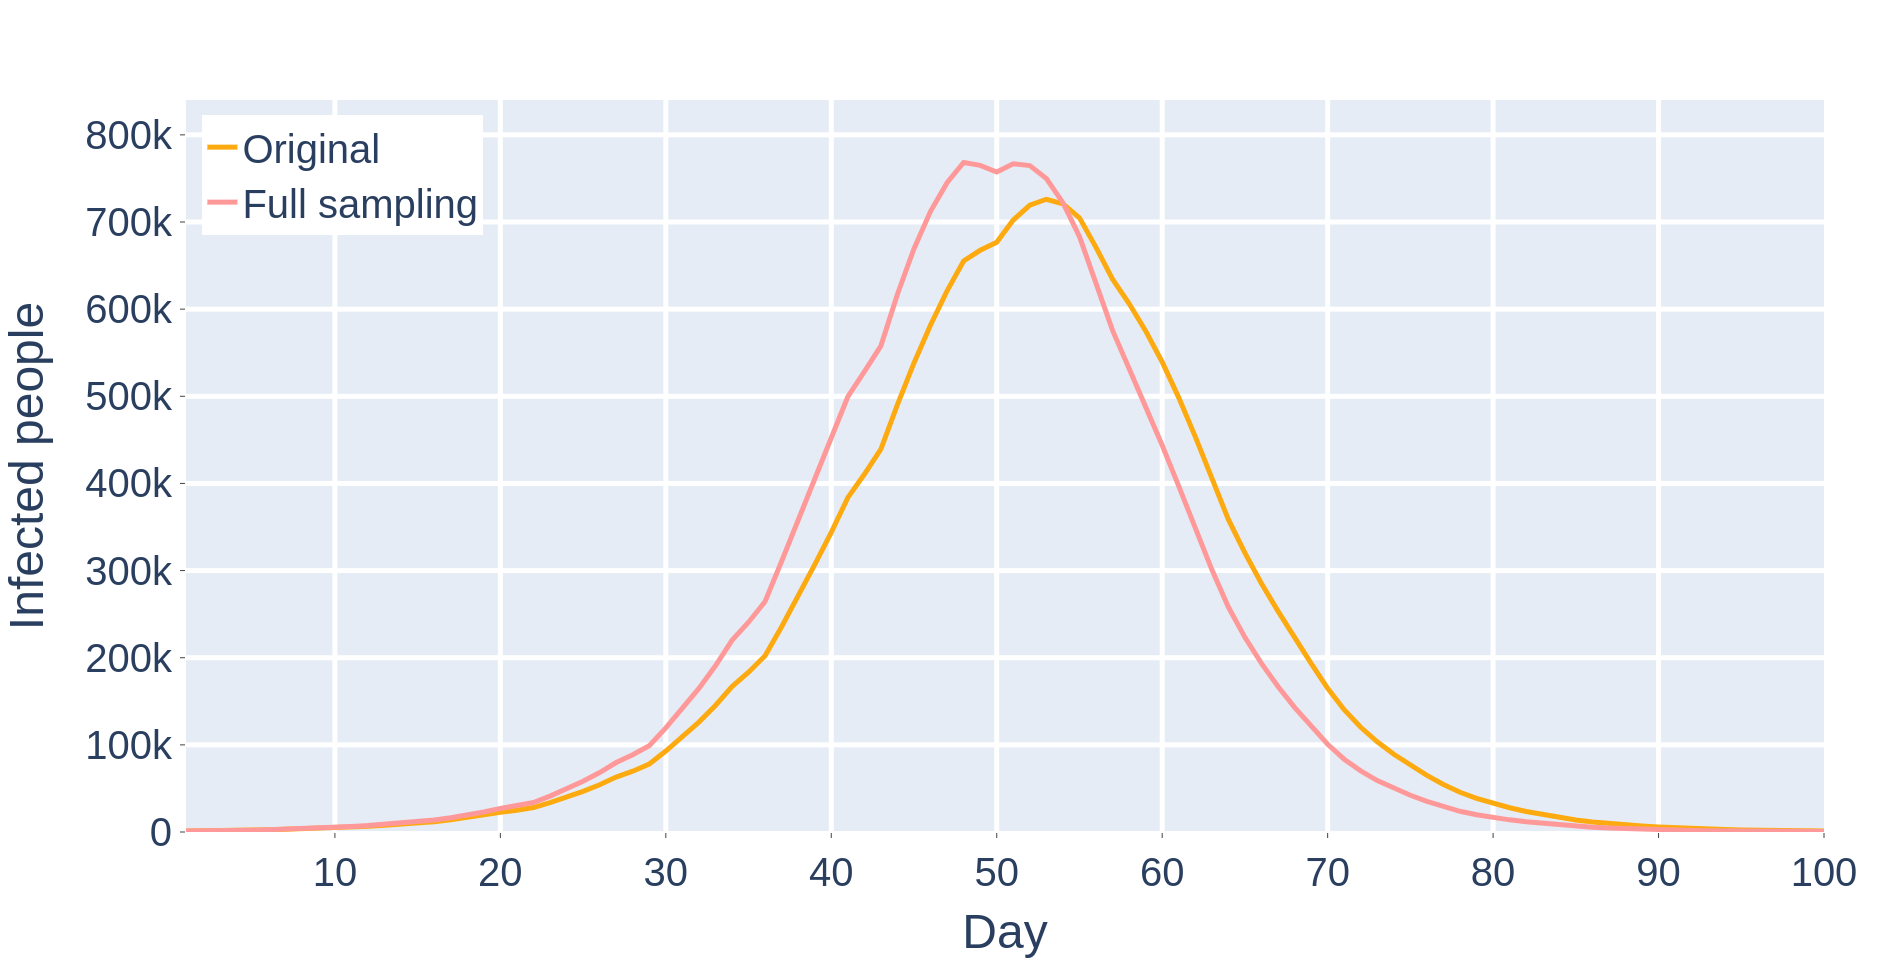
\includegraphics[width=.8\linewidth]{4 - Sampling/fig/full_sampling/infections_full_sampling.png}
    \caption{The number of infected people per day using the original \textsc{All-to-All} and \textsc{Full-sampling}. Simulations run on 11M population for 100 days without holidays using 1 thread (configurations in Appendix \ref{appendix:configurations}).}
    \label{fig:infections_full_sampling}
\end{figure}

\begin{figure}
    \centering
    \begin{subfigure}{.8\linewidth}
        \centering
        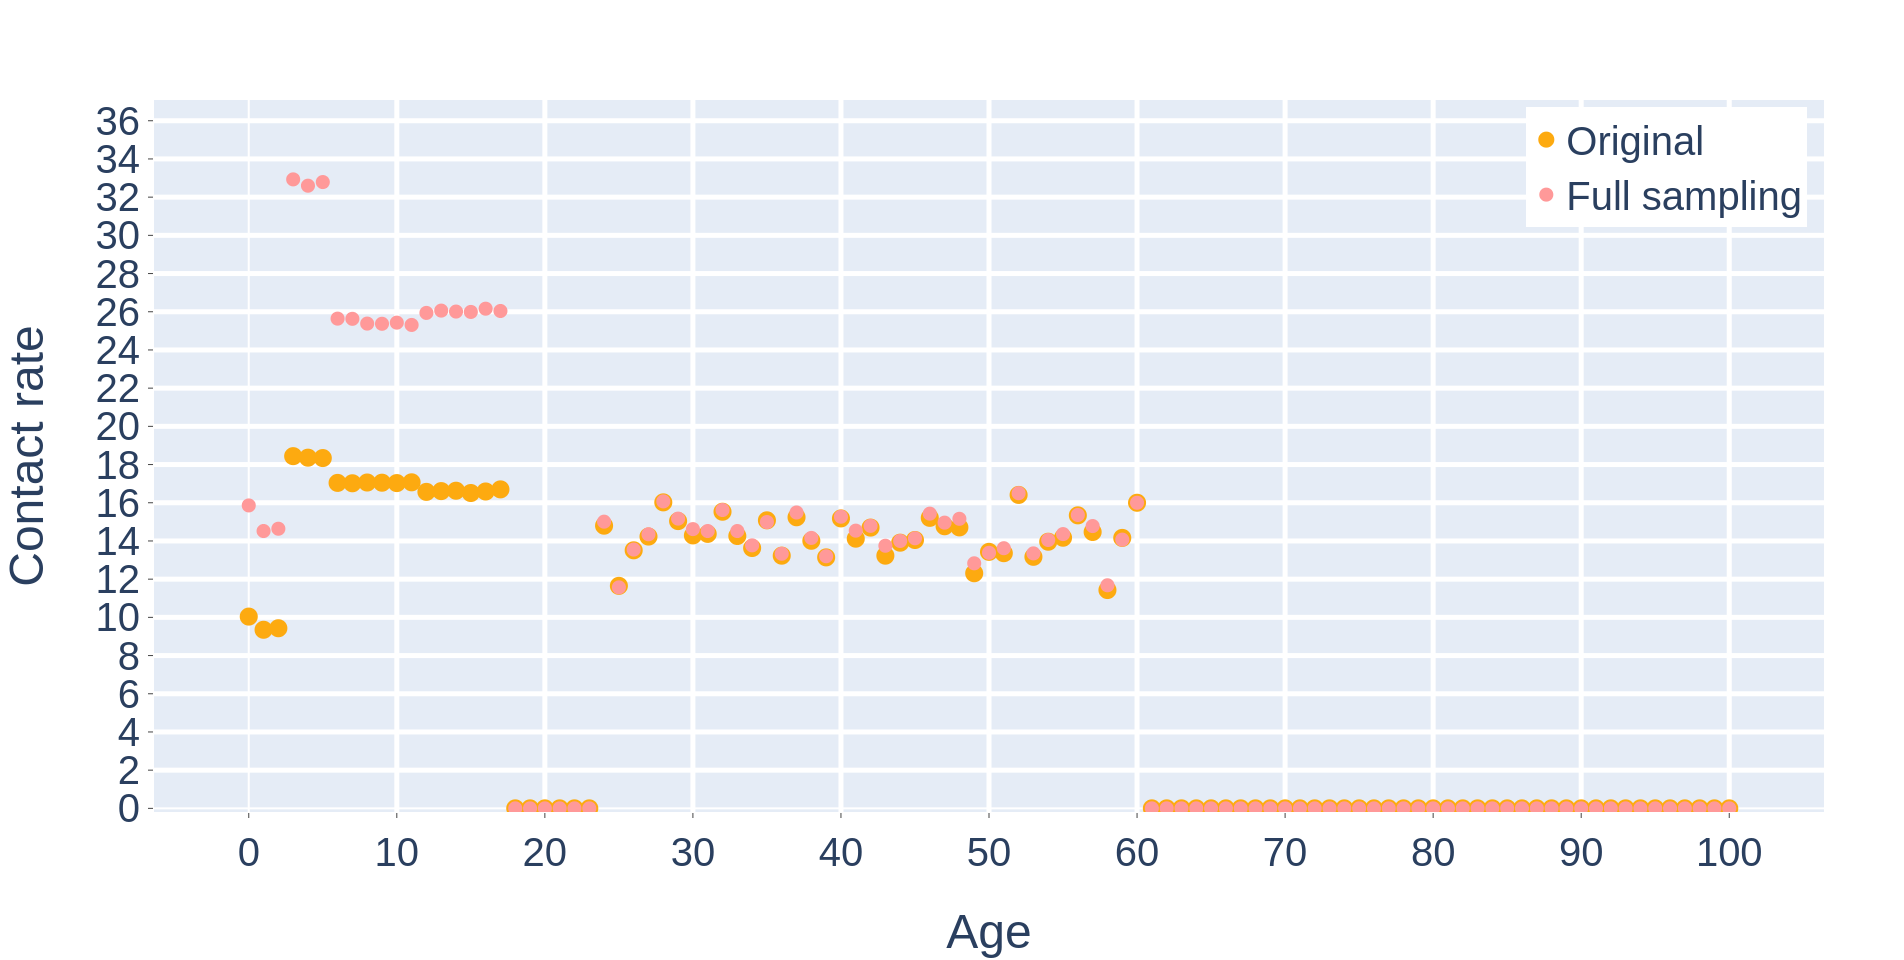
\includegraphics[width=\textwidth]{4 - Sampling/fig/full_sampling/fs_pType_vs_standard_reverse_cr_k12school.png}
        \caption{K-12 school}
        \label{fig:fs_pType_vs_standard_reversed_cr_k12school}
    \end{subfigure}
    \begin{subfigure}{.8\linewidth}
        \centering
        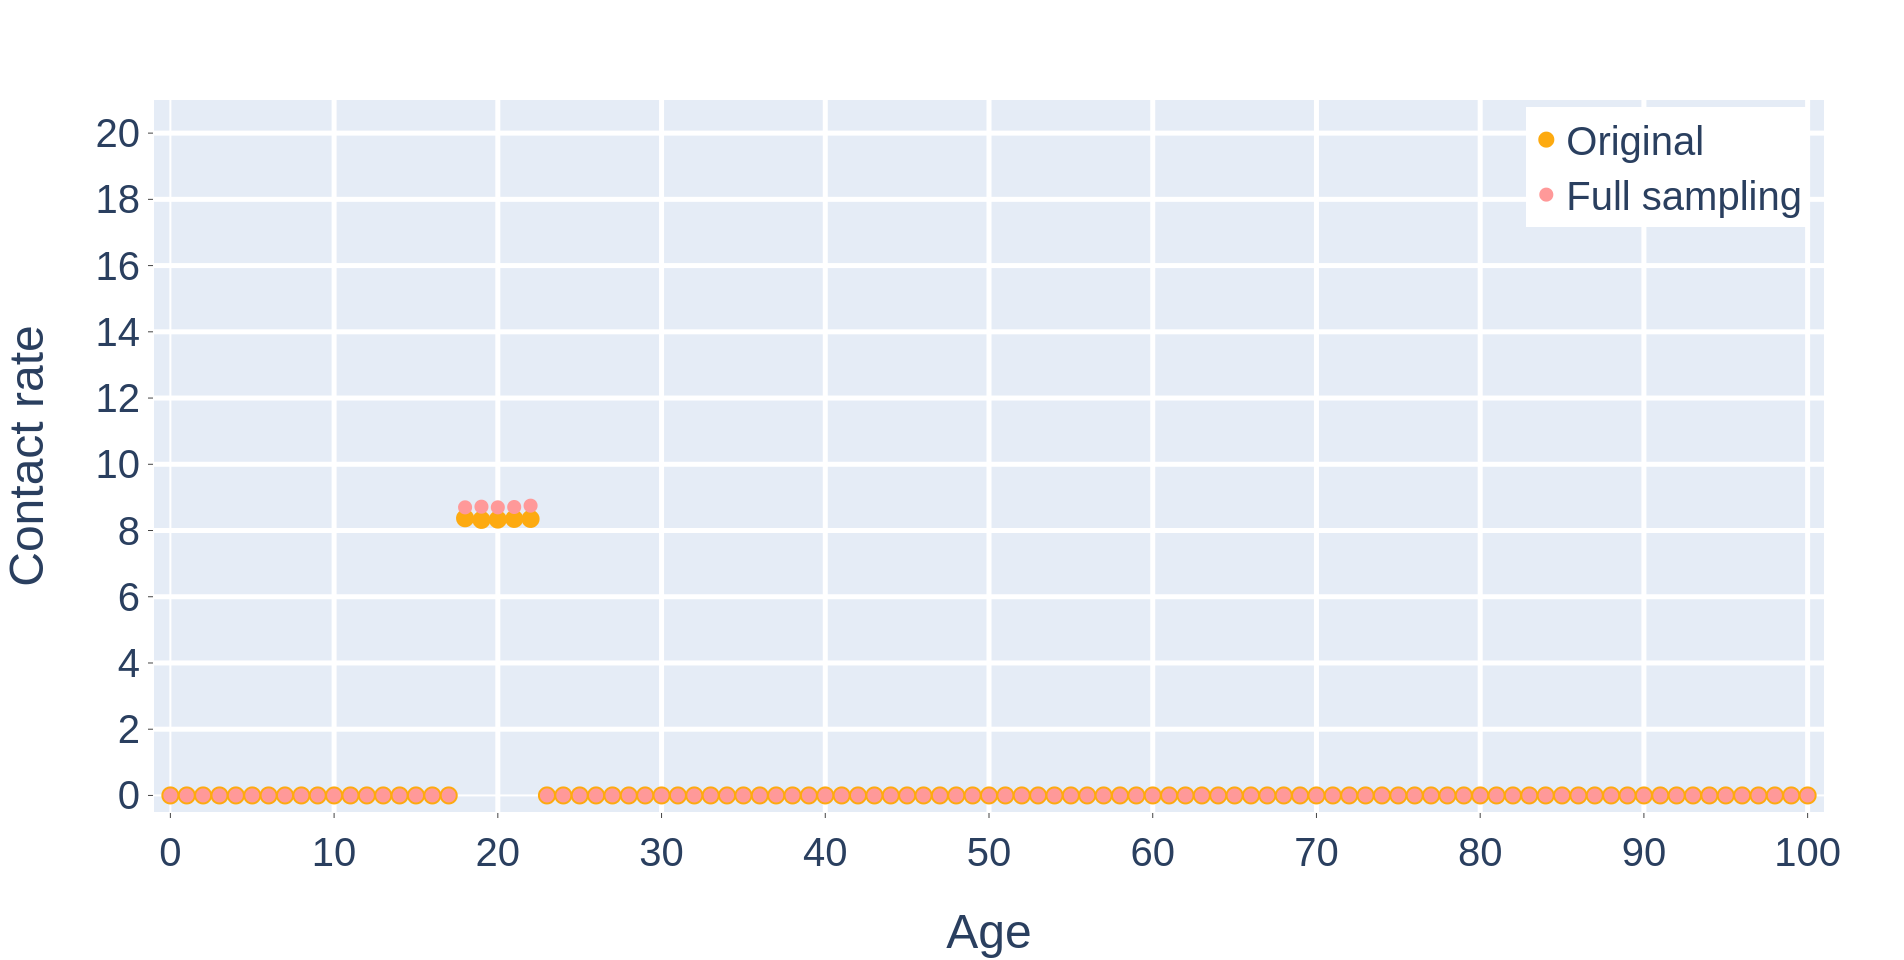
\includegraphics[width=\textwidth]{4 - Sampling/fig/full_sampling/fs_pType_vs_standard_reverse_cr_college.png}
        \caption{College}
        \label{fig:fs_pType_vs_standard_reversed_cr_college}
    \end{subfigure}
    \begin{subfigure}{.8\linewidth}
        \centering
        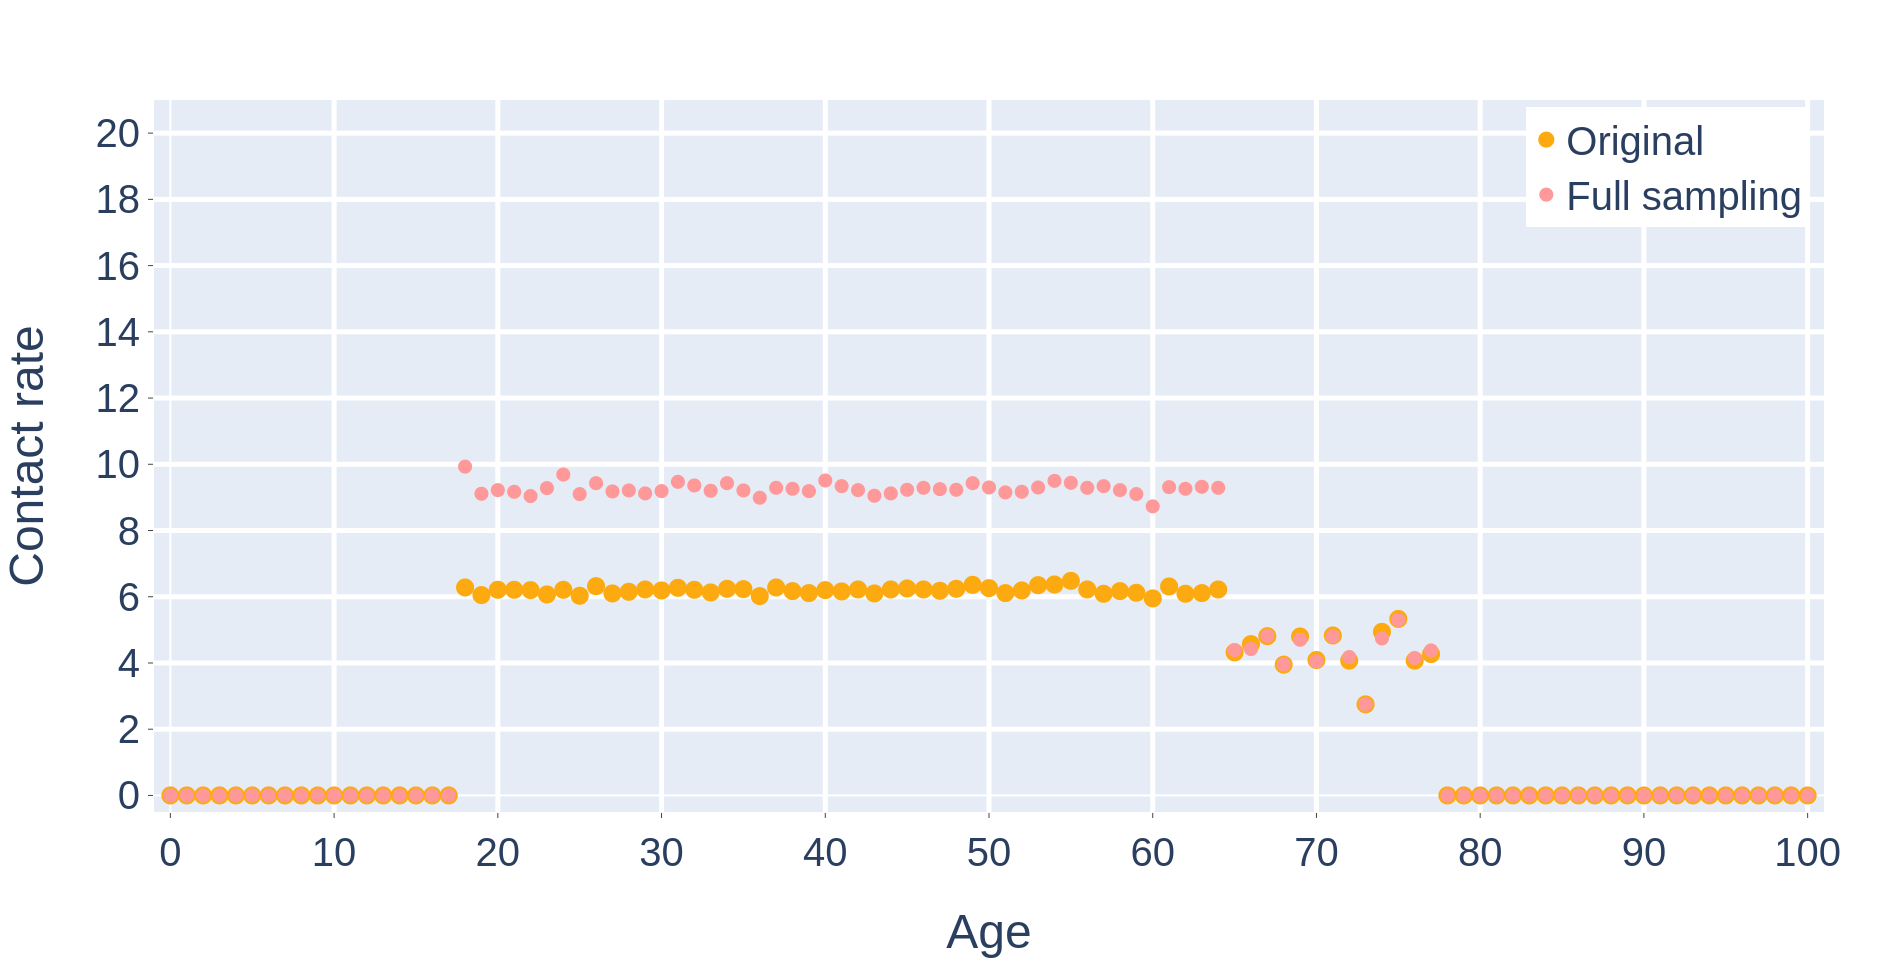
\includegraphics[width=\textwidth]{4 - Sampling/fig/full_sampling/fs_pType_vs_standard_reverse_cr_workplace.png}
        \caption{Workplace}
        \label{fig:fs_pType_vs_standard_reversed_cr_workplace}
    \end{subfigure}
    \caption{The reversed contact rates of \textsc{Full-sampling} compared to the original \textsc{All-to-All} reversed contact rates from Section \ref{subsec:reversed_contact_vector}.}
\end{figure}
\begin{figure}\ContinuedFloat
    \centering
    \begin{subfigure}{.8\linewidth}
        \centering
        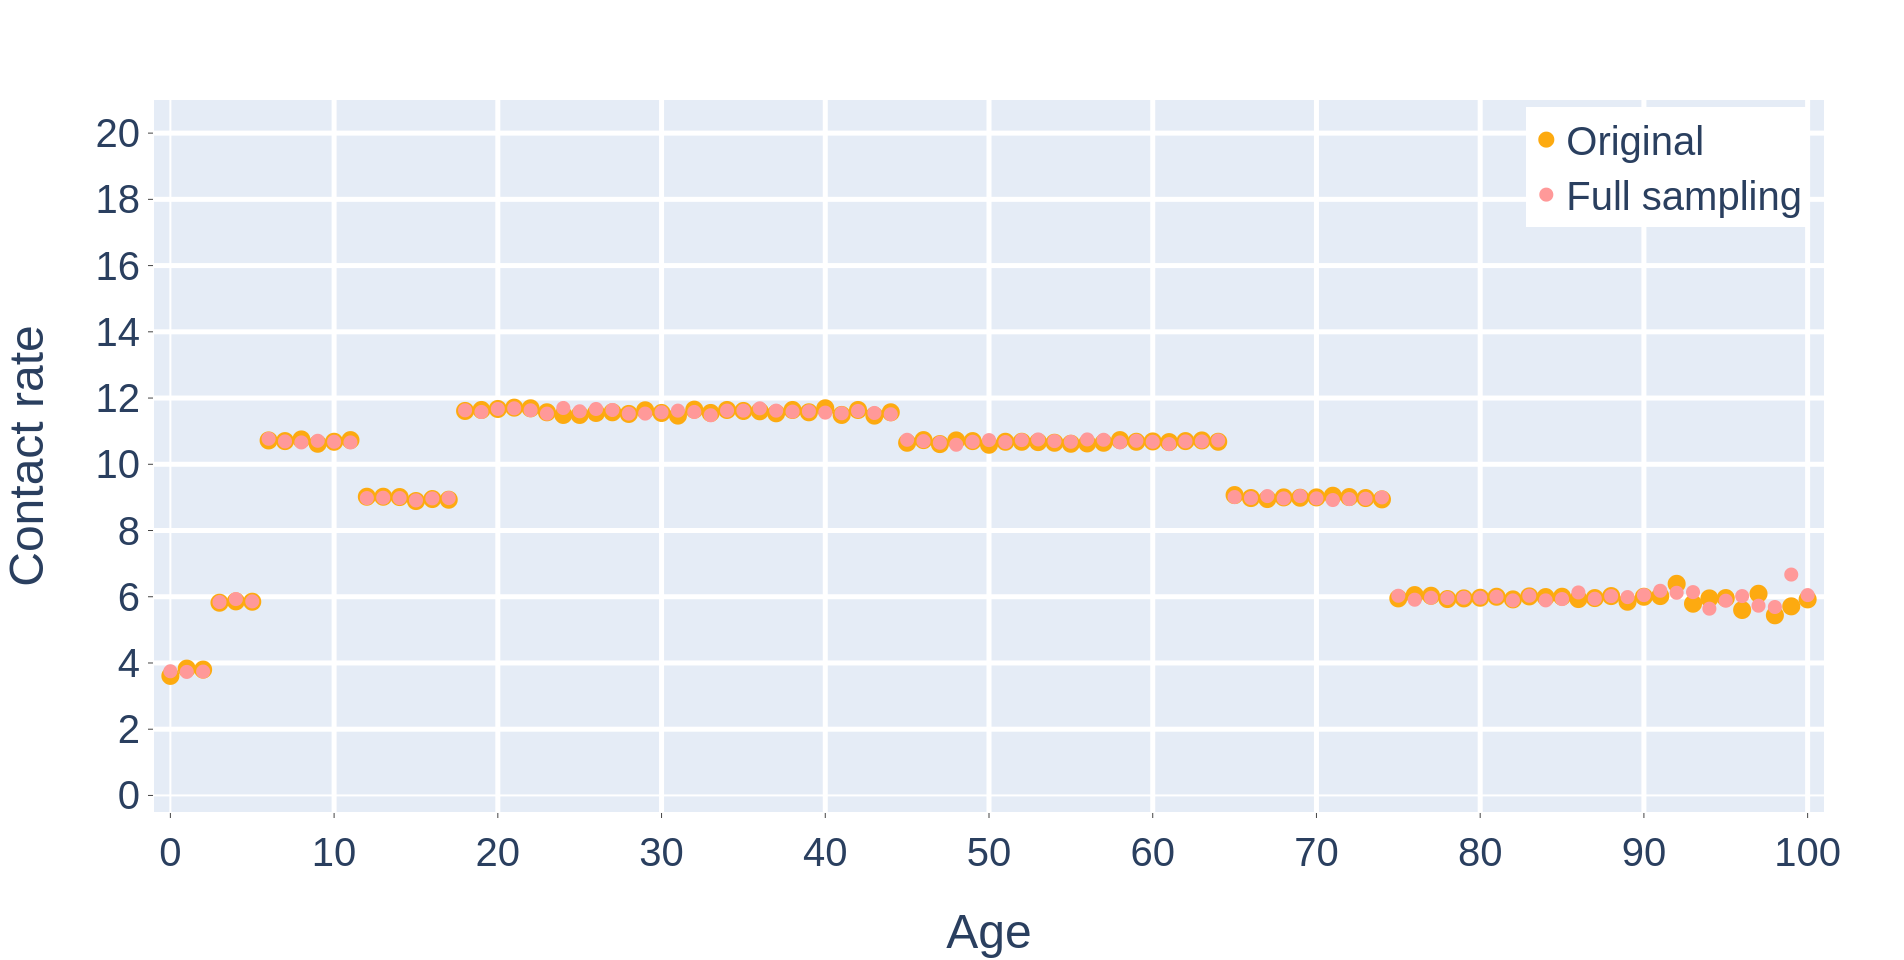
\includegraphics[width=\textwidth]{4 - Sampling/fig/full_sampling/fs_pType_vs_standard_reverse_cr_primary.png}
        \caption{Primary community}
        \label{fig:fs_pType_vs_standard_reversed_cr_primary}
    \end{subfigure}
    \begin{subfigure}{.8\linewidth}
        \centering
        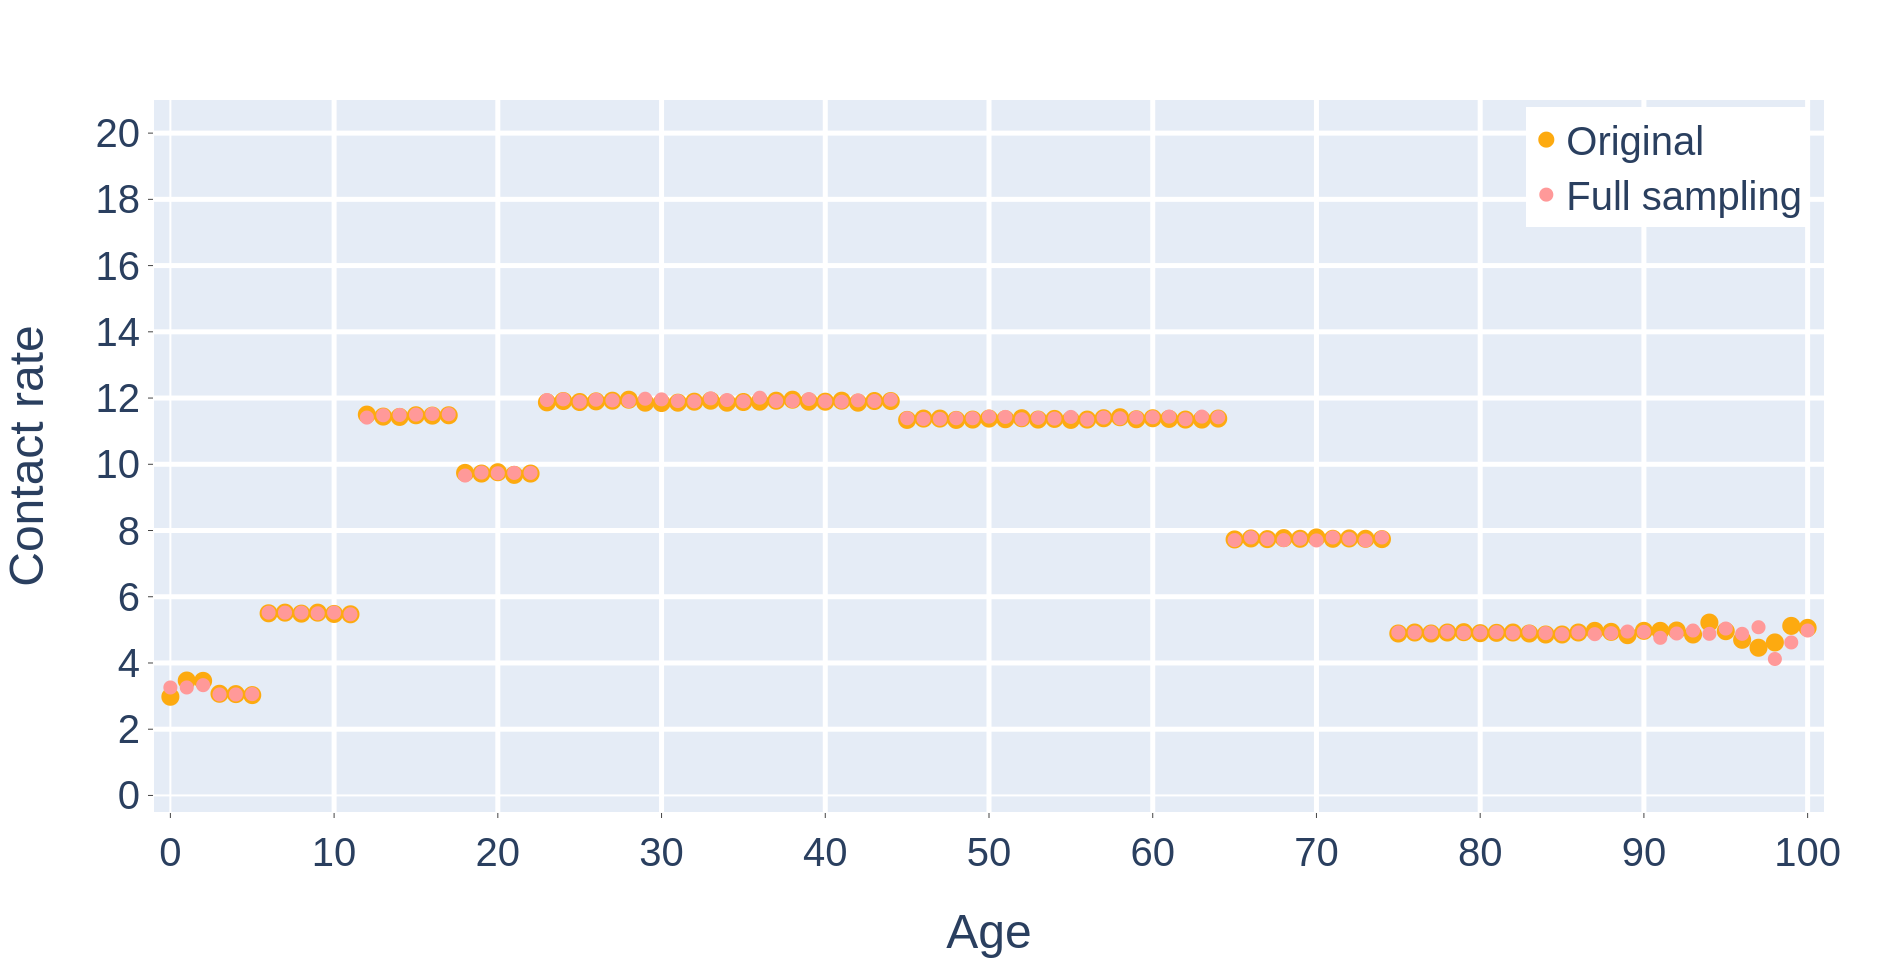
\includegraphics[width=\textwidth]{4 - Sampling/fig/full_sampling/fs_pType_vs_standard_reverse_cr_secondary.png}
        \caption{Secondary community}
        \label{fig:fs_pType_vs_standard_reversed_cr_secondary}
    \end{subfigure}
    \caption{The reversed contact rates of \textsc{Full-sampling} compared to the original \textsc{All-to-All} reversed contact rates from Section \ref{subsec:reversed_contact_vector}.}
    \label{fig:fs_pType_vs_standard_reversed_cr}
\end{figure}

\subsection{Performance}
\label{subsec:performance_full_sampling}
Although the \textsc{Full-sampling} algorithm is not generating valid results, we are still interested in its performance. Figure \ref{fig:fs_pType_vs_rest_infector} shows that it is faster than the original and \textsc{Iterative-intervals} approach. Compared to \textsc{Sampling-with-iteration}, it is remarkably slower on weekdays but faster on weekends. The speedup for the infector and total runtime compared to the original \textsc{All-to-All}, presented in Table \ref{tab:fs_pType_vs_standard_runtimes}, is respectively 2.30 and 2.21 which is less than \textsc{Sampling-with-iteration} that has speedups of 2.47 and 2.33.
\\\\
Since \textsc{Full-sampling} performs worse than expected, we further examine its results even though it is incorrect, because we can still gain valuable insights. In Figure \ref{fig:fs_pType_vs_rest_type_totals} we clearly see why \textsc{Full-sampling} is both better and worse than \textsc{Sampling-with-iteration} on different occasions. It needs significantly more time to compute the contacts in workplaces and even more time for K-12 schools. Nonetheless, the primary and secondary community pools slightly benefit from this faulty algorithm. If we look at Figure \ref{fig:times_avg_fs_pType_full}, we see that \textsc{Full-sampling} has the best runtimes for all larger pools, and that it has a linear time complexity for both communities as well as the workplace. So what we tried to achieve, namely speeding up same interval computations with sampling, has proven to be effective.
\\\\
Because the total runtime for the workplace is the worst of all while having such good results for larger pools, we also examine the results for smaller pool sizes in Figure \ref{fig:times_avg_fs_pType} for all types except the household. It can be seen that \textsc{Full-sampling} performs substantially worse on the K-12 school and college pools. For both community pools the algorithm performs slightly worse than \textsc{Sampling-with-iteration} for smaller pools. This, together with the effects on both school pools is due to the overhead that sampling has. \textsc{Full-sampling} becomes the fastest approach for workplace pools with approximately 150 people or more. For the community pools it has the best runtimes for pools with at least 250 people and performs better than the original for pools that contain 150 members or more. The algorithm thus works as expected for larger pools, but fails to perform in terms of speed on smaller pools.

\begin{figure}
    \centering
    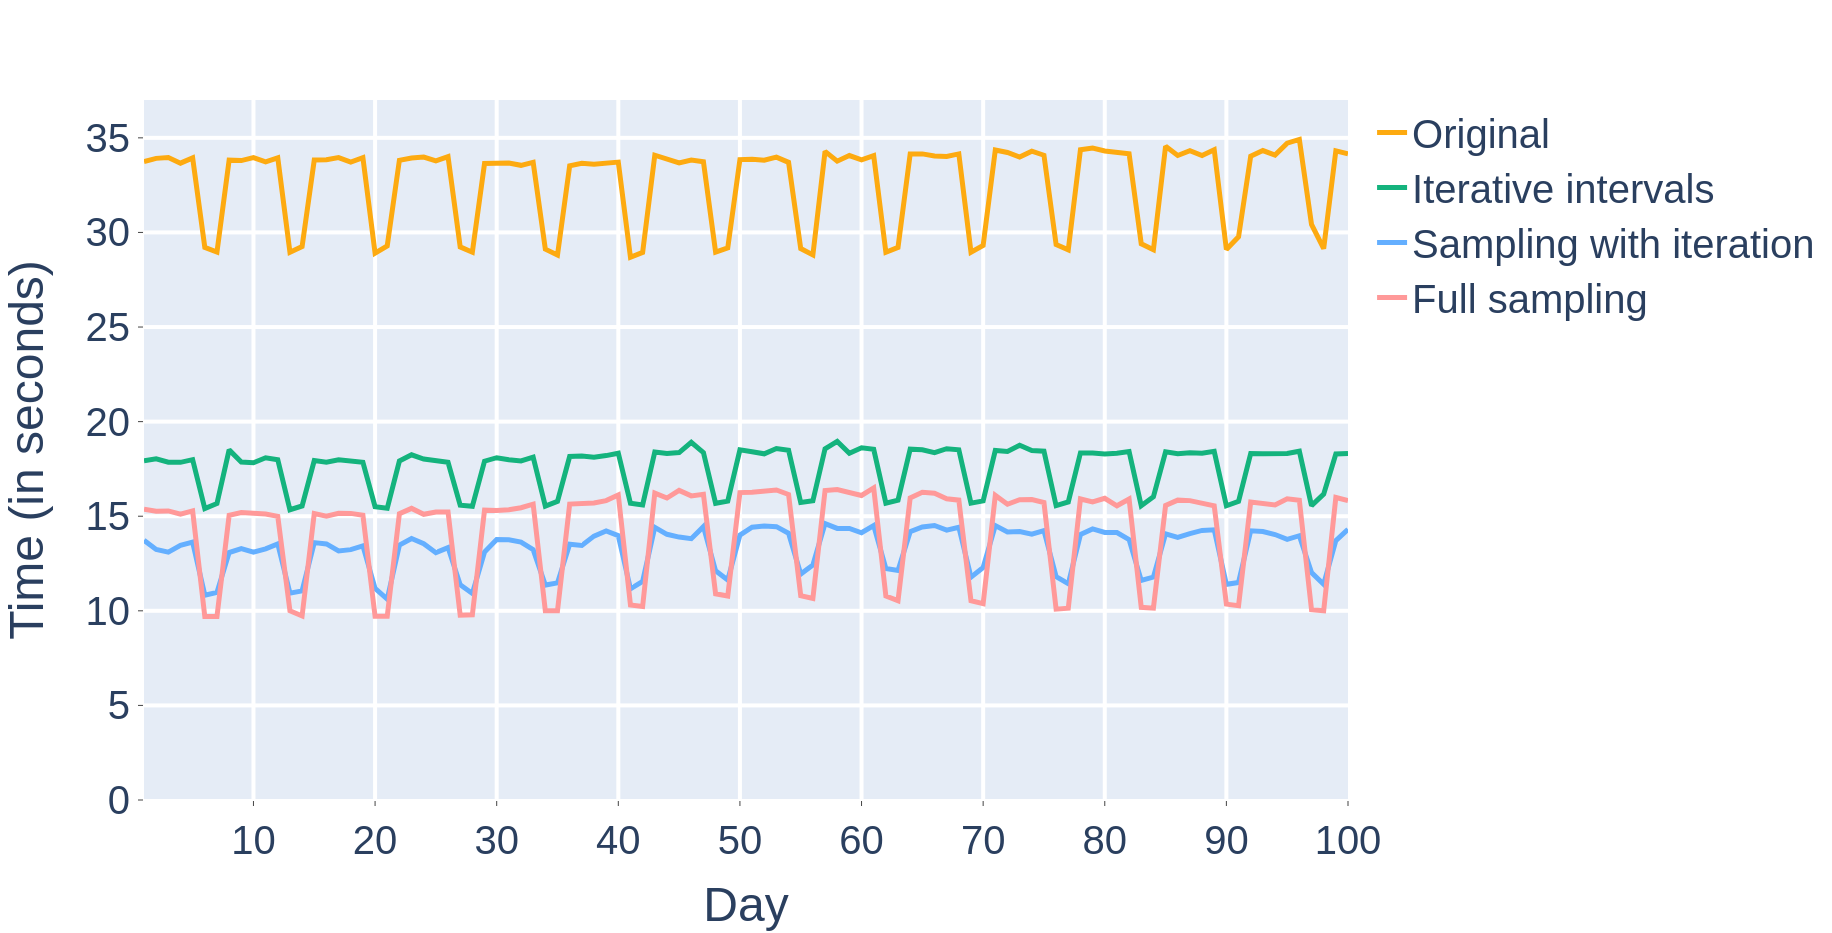
\includegraphics[width=\textwidth]{4 - Sampling/fig/full_sampling/fs_pType_vs_rest_infector.png}
    \caption{Comparison of the infector runtimes between \textsc{Full-sampling} and the other approaches. Simulations run on 11M population for 100 days without holidays using 1 thread (configurations in Appendix \ref{appendix:configurations}).}
    \label{fig:fs_pType_vs_rest_infector}
\end{figure}

\begin{table}
    \centering
    \begin{tabular}{@{}lrr@{}}
        \toprule
        \textsc{All-to-All} & Infector & Total \\ \midrule
        original & 32.63 & 33.77 \\
        full sampling & 14.16 & 15.30 \\ \hdashline[1pt/1pt]
        speedup & 2.30 & 2.21 \\ \bottomrule
    \end{tabular}
    \caption{Comparison of the average daily runtimes between the original and \textsc{Full-sampling} approach. Simulations run on 11M population for 100 days without holidays using 1 thread (configurations in Appendix \ref{appendix:configurations}).}
    \label{tab:fs_pType_vs_standard_runtimes}
\end{table}

\begin{figure}
    \centering
    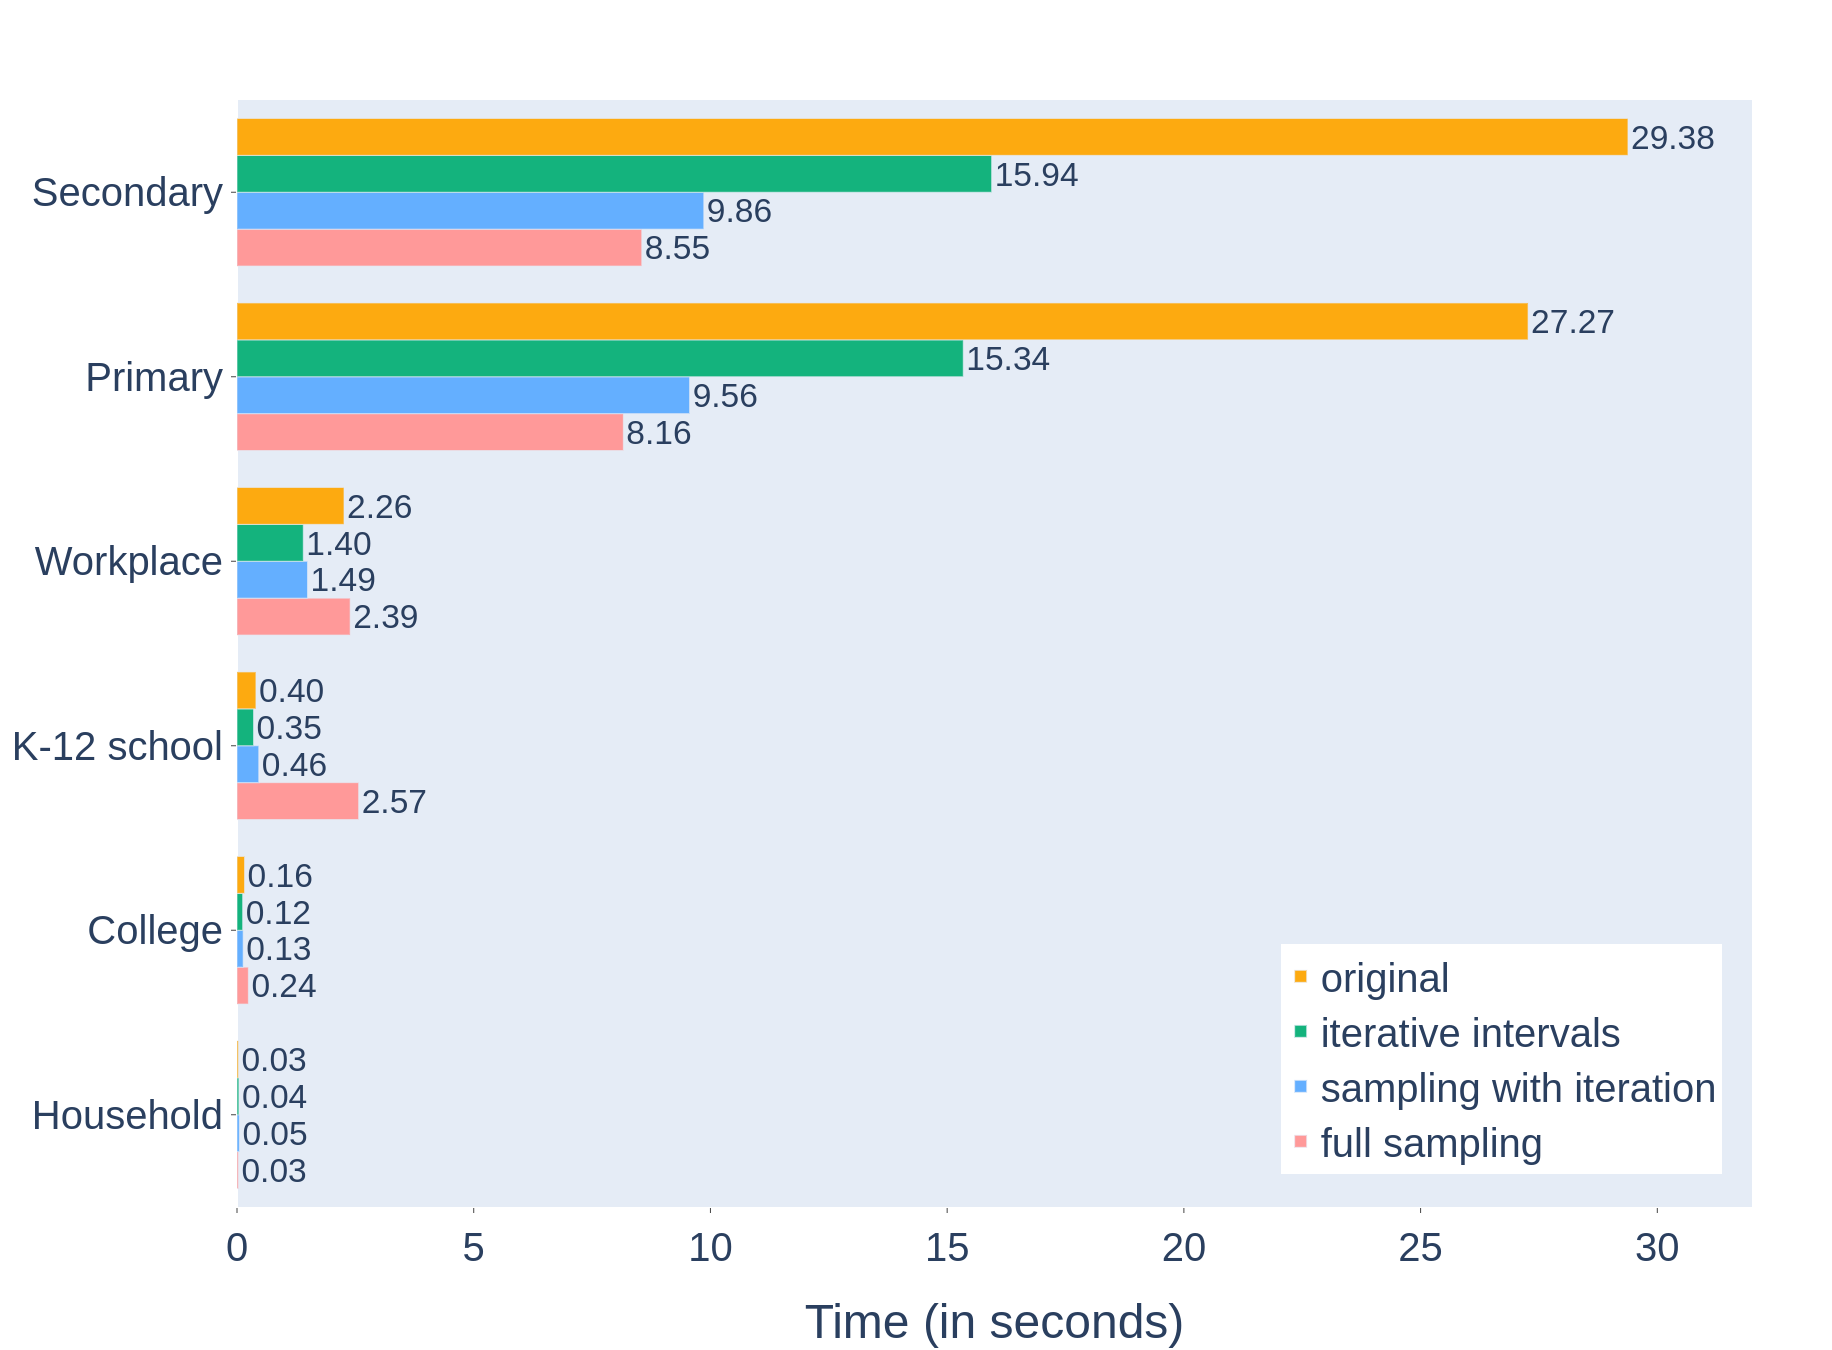
\includegraphics[width=\linewidth]{4 - Sampling/fig/full_sampling/fs_pType_vs_rest_type_totals.png}
    \caption{Comparison of the total infector runtimes (in seconds) per pool type on a day in which its pools are active. Simulations run on 11M population for 100 days without holidays using 1 thread (configurations in Appendix \ref{appendix:configurations}).}
    \label{fig:fs_pType_vs_rest_type_totals}
\end{figure}

\begin{figure}
    \centering
    \begin{subfigure}{.8\linewidth}
        \centering
        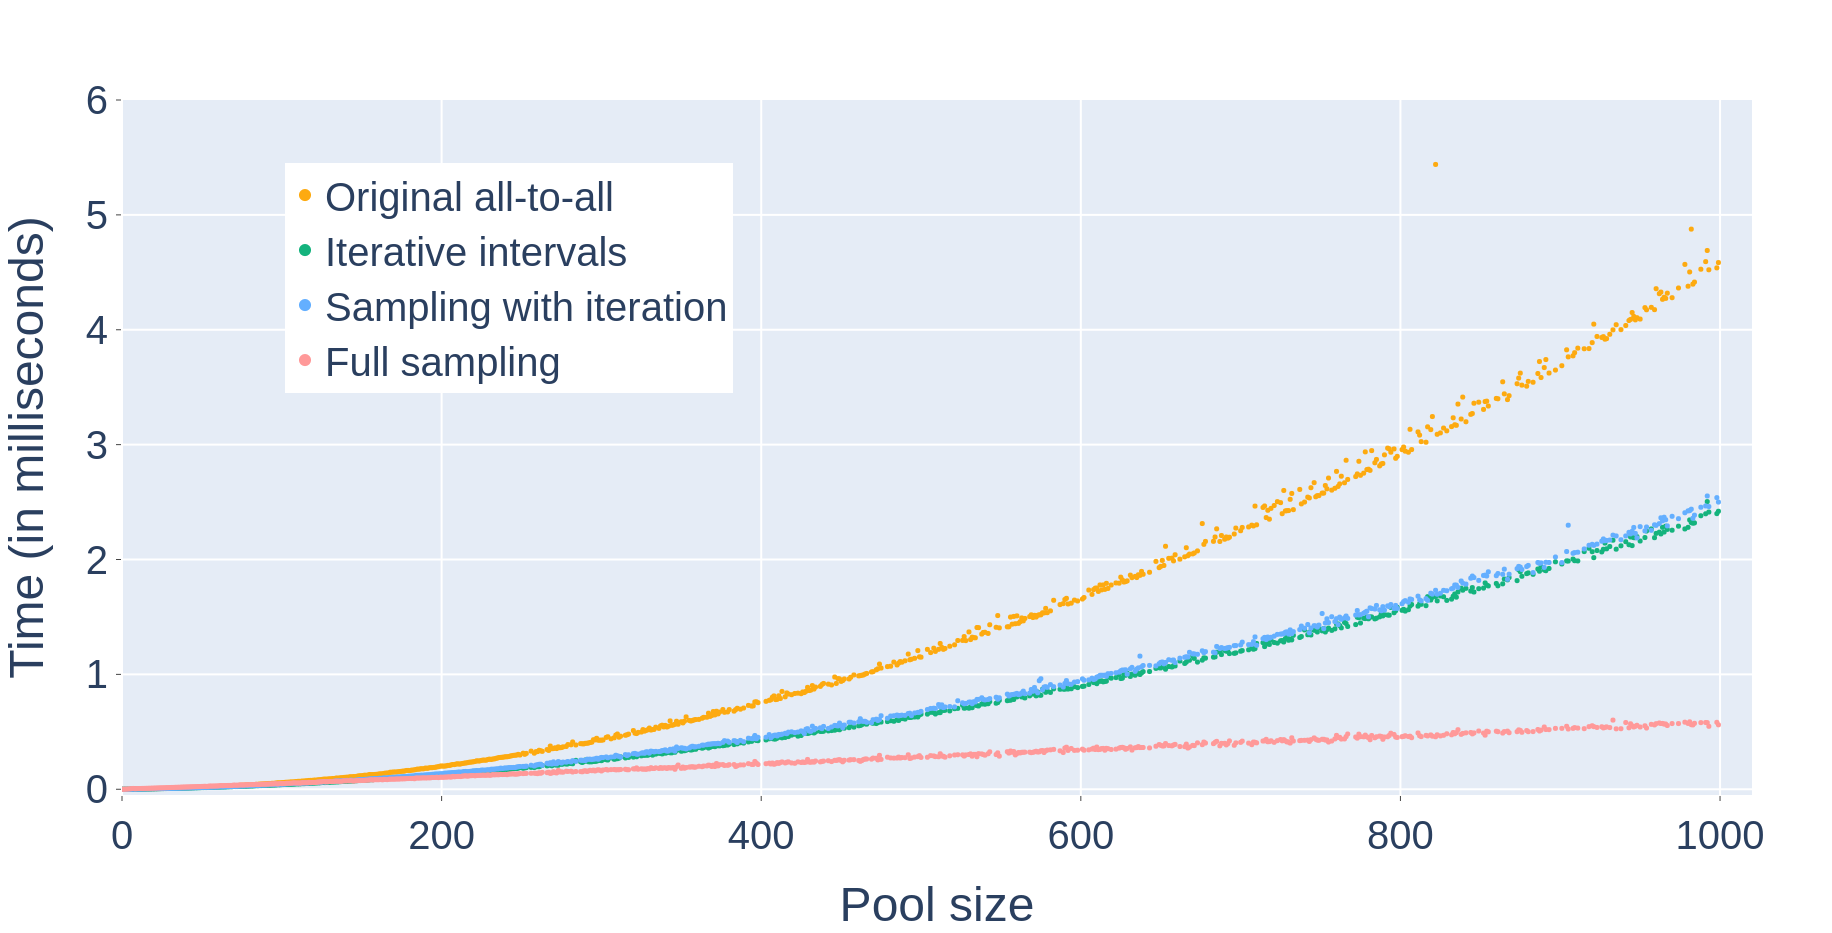
\includegraphics[width=\textwidth]{4 - Sampling/fig/full_sampling/times_avg_fs_pType_workplace_full.png}
        \caption{Workplace}
        \label{fig:times_avg_fs_pType_workplace_full}
    \end{subfigure}
    \begin{subfigure}{.8\linewidth}
        \centering
        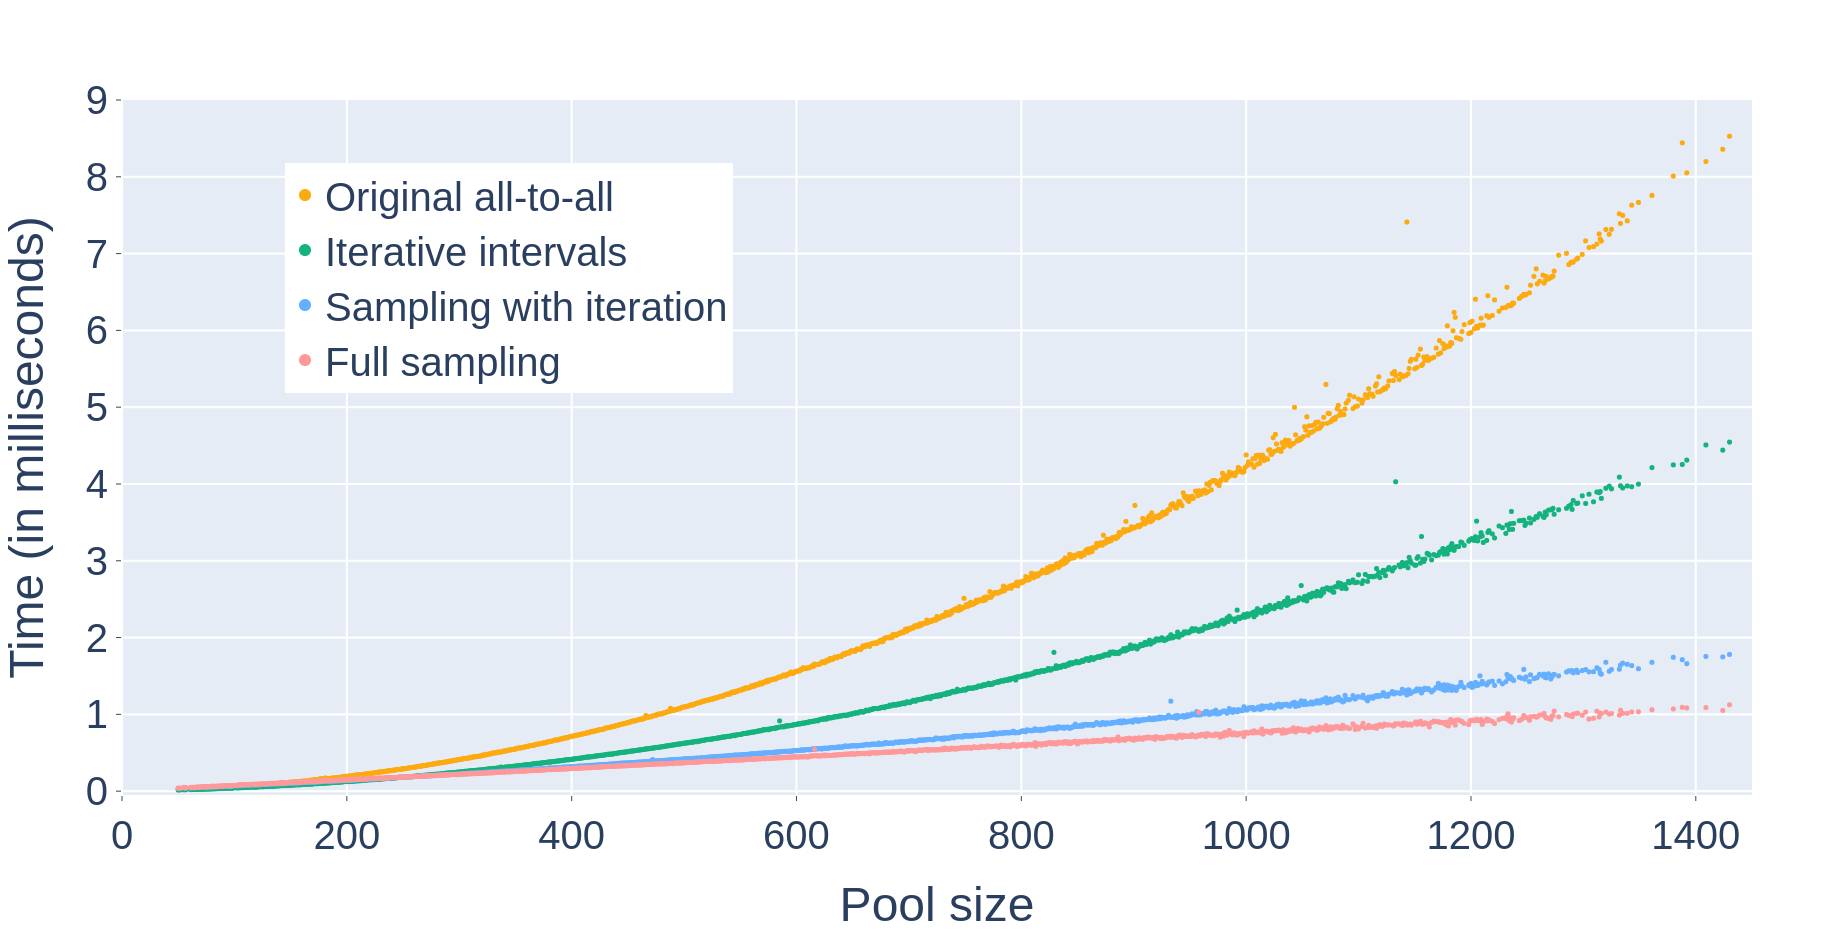
\includegraphics[width=\textwidth]{4 - Sampling/fig/full_sampling/times_avg_fs_pType_primary_full.png}
        \caption{Primary community}
        \label{fig:times_avg_fs_pType_primary_full}
    \end{subfigure}
    \begin{subfigure}{.8\linewidth}
        \centering
        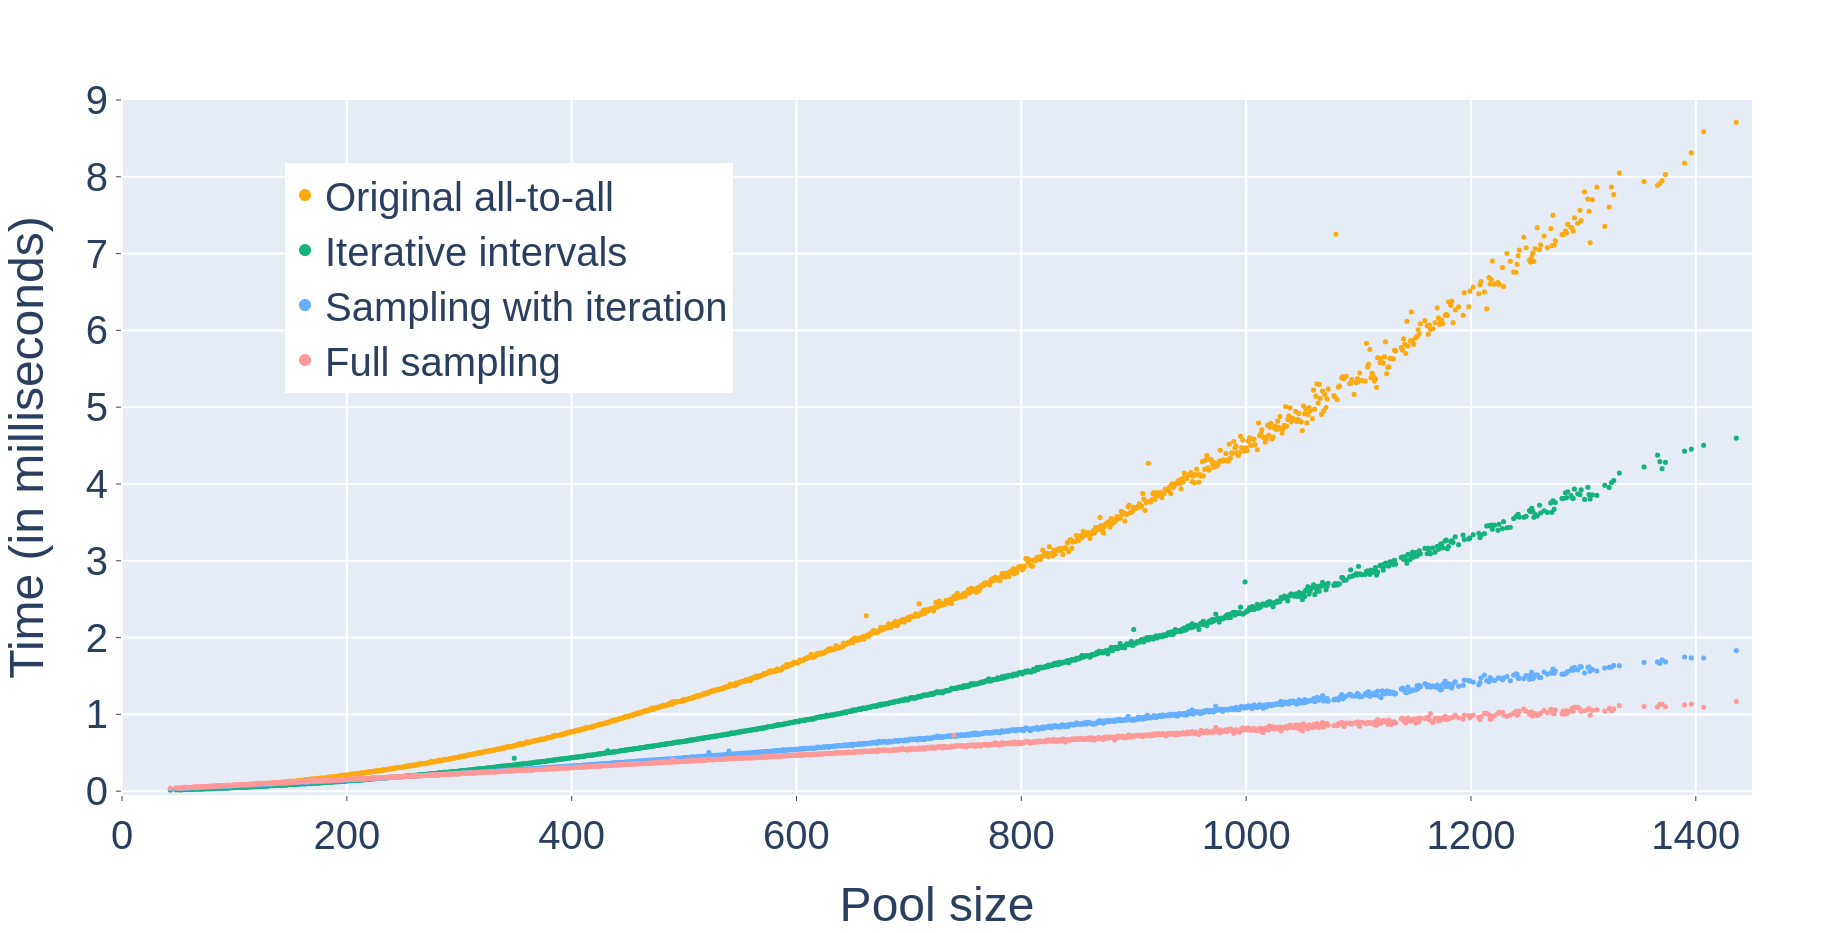
\includegraphics[width=\textwidth]{4 - Sampling/fig/full_sampling/times_avg_fs_pType_secondary_full.png}
        \caption{Secondary community}
        \label{fig:times_avg_fs_pType_secondary_full}
    \end{subfigure}
    \caption{Average infector runtimes (in milliseconds) per pool size using different approaches. Simulations run on 11M population for 100 days without holidays using 1 thread (configurations in Appendix \ref{appendix:configurations}).}
    \label{fig:times_avg_fs_pType_full}
\end{figure}

\begin{figure}
    \centering
    \begin{subfigure}{.8\linewidth}
        \centering
        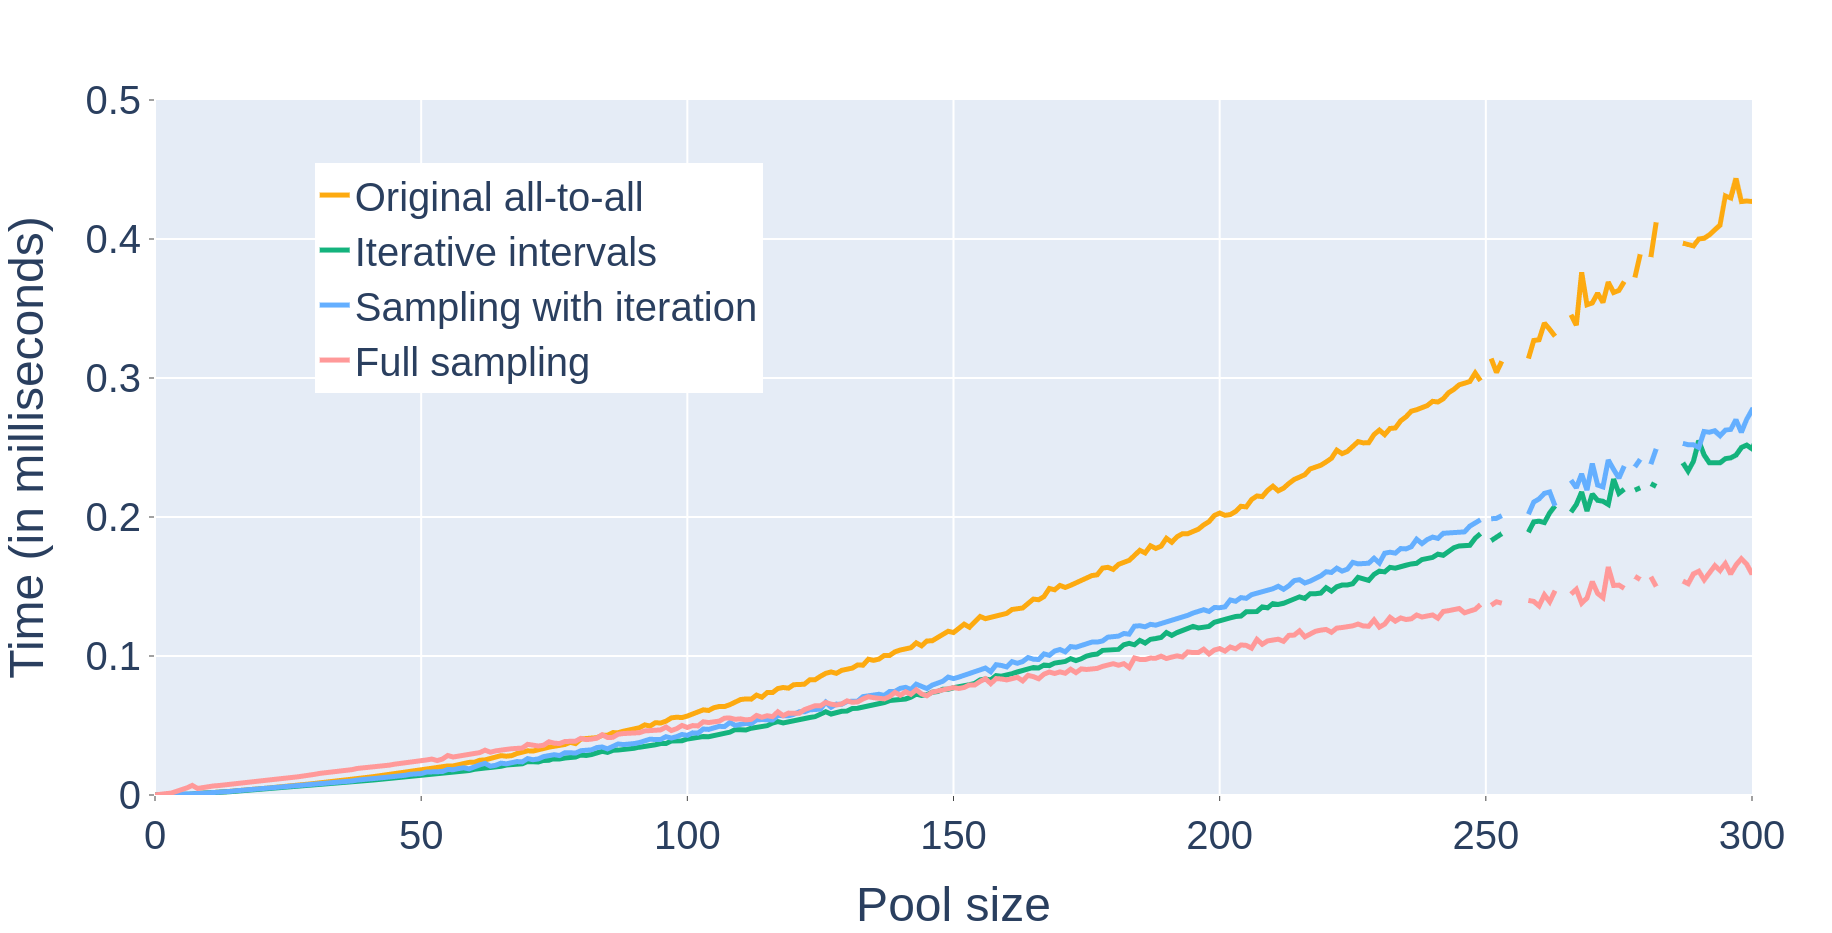
\includegraphics[width=\textwidth]{4 - Sampling/fig/full_sampling/times_avg_fs_pType_workplace.png}
        \caption{Workplace pool sizes [0, 300]}
        \label{fig:times_avg_fs_pType_workplace}
    \end{subfigure}
    \begin{subfigure}{.8\linewidth}
        \centering
        \includegraphics[width=\textwidth]{4 - Sampling/fig/full_sampling/times_avg_fs_pType_primary.png}
        \caption{Primary community pool sizes [0, 300]}
        \label{fig:times_avg_fs_pType_primary}
    \end{subfigure}
    \begin{subfigure}{.8\linewidth}
        \centering
        \includegraphics[width=\textwidth]{4 - Sampling/fig/full_sampling/times_avg_fs_pType_secondary.png}
        \caption{Secondary community pool sizes [0, 300]}
        \label{fig:times_avg_fs_pType_secondary}
    \end{subfigure}
    \caption{Average infector runtimes per pool size using different approaches. Simulations run on 11M population for 100 days without holidays using 1 thread (configurations in Appendix \ref{appendix:configurations}).}
\end{figure}
\begin{figure}\ContinuedFloat
    \centering
    \begin{subfigure}{.8\linewidth}
        \centering
        \includegraphics[width=\textwidth]{4 - Sampling/fig/full_sampling/times_avg_fs_pType_k12school.png}
        \caption{K-12 school}
        \label{fig:times_avg_fs_pType_k12school}
    \end{subfigure}
    \begin{subfigure}{.8\linewidth}
        \centering
        \includegraphics[width=\textwidth]{4 - Sampling/fig/full_sampling/times_avg_fs_pType_college.png}
        \caption{College}
        \label{fig:times_avg_fs_pType_college}
    \end{subfigure}
    \caption{Average infector runtimes per pool size using different approaches. Simulations run on 11M population for 100 days without holidays using 1 thread (configurations in Appendix \ref{appendix:configurations}).}
    \label{fig:times_avg_fs_pType}
\end{figure}

\section{Full sampling (>150)}
\label{sec:adjusted_full_sampling}
Examining the correctness of \textsc{Full-sampling} in Section \ref{subsec:correctness_fs} taught us that it produces too much contacts for workplace and K-12 school pools and a little bit too much for college pools. The primary and secondary communities, on the other hand, generate a valid amount of contacts. The reason for these incorrect contact rates are the duplicate contacts, which we handle like they are valid contacts like the rest. The proof in Appendix \ref{appendix:sampling_same_interval} considers a contact to be symmetric, which means that duplicate contacts should be considered as only one unique contact. Pool types that have these large, incorrect contact rates do not contain pools with more than 50 people and 94\% of workplace pools contain only 1 to 9 persons. These are also the pools in which there are only a few intervals and most of them are in the same interval. This is the reason that there are so many duplicate contacts for these types, especially K-12 schools where the original contact rates are very high. Because these pools are small and because most of the people are in the same interval, the probability of getting duplicate contacts is very high.
\\\\
Although registering too many contacts does no harm, what happens after every duplicate contact is the reason that our approach fails the tests. When there is contact between two individuals, we check if transmission can occur. The duplicate contact does the exact same thing and also checks if transmission can occur. Thus, when we performed the Bernoulli trial for transmission the first time and it failed, the duplicate contact creates a second chance for the susceptible person to become exposed. This is the reason that the number of infected people in Figure \ref{fig:infections_full_sampling} is higher than it should be, because the probability of getting infected by someone in the same interval is sometimes doubled.
\\\\
Eliminating the duplicate contacts should thus correct the \textsc{Full-sampling} algorithm, but this would require us to keep track of the contacts that have already been sampled. This will be discussed in Section \ref{sec:full_sampling_unique_contacts}. For now we, want to see if we can reduce the number of duplicate contacts without explicitly checking for them. We just pointed out that those duplicates occur more the smaller the interval. Therefore, using \textsc{Full-sampling} only on larger pools, which have a smaller chance of generating duplicate contacts, could solve the problem. Since Section \ref{subsec:performance_full_sampling} revealed that our approach becomes faster than the original for community pools with at least 150 people, we set this as a threshold to decide of a pool uses the original \textsc{All-to-All} algorithm or \textsc{Full-sampling}. We will call this new approach \textsc{Full-sampling (>150)}, because it uses the same implementation as described in Algorithm \ref{alg:full_sampling}, but with the alteration to the if-test to check for pools with less than 150 people instead of checking for households.

\subsection{Correctness}
\label{subsec:correctness_adjusted_full_sampling}
To check if our \textsc{Full-sampling (>150)} approach works, we execute the built-in tests that it previously failed. This time, the algorithm passes every test which indicates that its results can be considered valid. The reversed contact rates in Figure \ref{fig:fs_pSize_vs_standard_reversed_cr} also show that our adjustment results in our algorithm to produce the right amount of contacts. Even though the algorithm now passes the tests, we know that its results are not 100\% correct because it still allows duplicate contacts to happen that lead to double probability of transmission. Because we only apply our algorithm to pools with at least 150 members, duplicate contacts have a smaller probability to occur. Setting the threshold even higher would naturally increase the correctness of the results. With our current threshold of 150, we can say that the \textsc{Full-sampling (>150)} approach is a valid \textsc{All-to-All} infector algorithm as long as we accept the fact that its results are nearly 100\% correct. There is thus a trade off that has to be made regarding performance versus precision.

\begin{figure}
    \centering
    \begin{subfigure}{.8\linewidth}
        \centering
        \includegraphics[width=\textwidth]{4 - Sampling/fig/adjusted_full_sampling/fs_pSize_vs_standard_reverse_cr_k12school.png}
        \caption{K-12 school}
        \label{fig:fs_pSize_vs_standard_reversed_cr_k12school}
    \end{subfigure}
    \begin{subfigure}{.8\linewidth}
        \centering
        \includegraphics[width=\textwidth]{4 - Sampling/fig/adjusted_full_sampling/fs_pSize_vs_standard_reverse_cr_college.png}
        \caption{College}
        \label{fig:fs_pSize_vs_standard_reversed_cr_college}
    \end{subfigure}
    \begin{subfigure}{.8\linewidth}
        \centering
        \includegraphics[width=\textwidth]{4 - Sampling/fig/adjusted_full_sampling/fs_pSize_vs_standard_reverse_cr_workplace.png}
        \caption{Workplace}
        \label{fig:fs_pSize_vs_standard_reversed_cr_workplace}
    \end{subfigure}
    \caption{The reversed contact rates of \textsc{Full-sampling (>150)} compared to the original \textsc{All-to-All} reversed contact rates from Section \ref{subsec:reversed_contact_vector}.}
\end{figure}
\begin{figure}\ContinuedFloat
    \centering
    \begin{subfigure}{.8\linewidth}
        \centering
        \includegraphics[width=\textwidth]{4 - Sampling/fig/adjusted_full_sampling/fs_pSize_vs_standard_reverse_cr_primary.png}
        \caption{Primary community}
        \label{fig:fs_pSize_vs_standard_reversed_cr_primary}
    \end{subfigure}
    \begin{subfigure}{.8\linewidth}
        \centering
        \includegraphics[width=\textwidth]{4 - Sampling/fig/adjusted_full_sampling/fs_pSize_vs_standard_reverse_cr_secondary.png}
        \caption{Secondary community}
        \label{fig:fs_pSize_vs_standard_reversed_cr_secondary}
    \end{subfigure}
    \caption{The reversed contact rates of \textsc{Full-sampling (>150)} compared to the original \textsc{All-to-All} reversed contact rates from Section \ref{subsec:reversed_contact_vector}.}
    \label{fig:fs_pSize_vs_standard_reversed_cr}
\end{figure}

\subsection{Performance}
\label{subsec:performance_adjusted_full_sampling}
Now that we created a legitimate algorithm, we are interested in how it performs. Figure \ref{fig:fs_pSize_vs_rest_infector} presents promising results where this new approach achieves the best results out of all of the valid infector algorithms. Table \ref{tab:fs_pSize_vs_standard_runtimes} confirms that \textsc{Full-sampling (>150)} reaches the fastest average infector and total runtimes and has thus the best speedup for these with respectively 2.75 and 2.60.
\\\\
Because we set out pool size threshold at 150, the K-12 school and college pools only use the original \textsc{All-to-All}. Figure \ref{fig:fs_pSize_vs_rest_type_totals} shows that this is indeed the case and that their infector runtimes are slightly higher than the original, which is due to the extra if-test of course. The most noticeable difference can be seen for the workplace, which has now by far the best runtimes using the \textsc{Full-sampling (>150)} method. The community pools both have lost a small amount of time compared to the erroneous \textsc{Full-sampling}, but they now still execute faster than \textsc{Sampling-with-iteration} by more than a second per day. In Section \ref{subsec:performance_full_sampling} we already discussed how \textsc{Full-sampling} performs per pool type in function of the pool sizes. If we were to visualize these results again, we would see that every pool type follows the curve of the original \textsc{All-to-All} and that pools with at least 150 members follow the \textsc{Full-sampling} line.

\begin{figure}
    \centering
    \includegraphics[width=\textwidth]{4 - Sampling/fig/adjusted_full_sampling/fs_pSize_vs_rest_infector.png}
    \caption{Comparison of the infector runtimes between \textsc{Full-sampling (>150)} and the other valid approaches. Simulations run on 11M population for 100 days without holidays using 1 thread (configurations in Appendix \ref{appendix:configurations}).}
    \label{fig:fs_pSize_vs_rest_infector}
\end{figure}

\begin{table}
    \centering
    \begin{tabular}{@{}lrr@{}}
        \toprule
        \textsc{All-to-All} & Infector & Total \\ \midrule
        original & 32.63 & 33.77 \\
        full sampling (\textgreater{}150) & 11.85 & 12.98 \\ \hdashline[1pt/1pt]
        speedup & 2.75 & 2.60 \\ \bottomrule
    \end{tabular}
    \caption{Comparison of the average daily runtimes between the original and \textsc{Full-sampling (>150)} approach. Simulations run on 11M population for 100 days without holidays using 1 thread (configurations in Appendix \ref{appendix:configurations}).}
    \label{tab:fs_pSize_vs_standard_runtimes}
\end{table}

\begin{figure}
    \centering
    \includegraphics[width=\linewidth]{4 - Sampling/fig/adjusted_full_sampling/fs_pSize_vs_rest_type_totals.png}
    \caption{Comparison of the total infector runtimes (in seconds) per pool type on a day in which its pools are active. Simulations run on 11M population for 100 days without holidays using 1 thread (configurations in Appendix \ref{appendix:configurations}).}
    \label{fig:fs_pSize_vs_rest_type_totals}
\end{figure}

\section{Full sampling unique contacts}
\label{sec:full_sampling_unique_contacts}
Previously we explained how duplicate contacts are the reason for our \textsc{Full-sampling} approach to be incorrect and \textsc{Full-sampling (>150)} to be not 100\% correct. Now we want to correct these approaches by verifying for every contact that it is unique. If a sampled contact turns out to be a duplicate, we count it as a valid contact but do not register it nor continue to determine transmission. Because we check the contacts to eliminate duplicates, this new approach will be called \textsc{Full-sampling-unique-contacts}.

\subsection{Implementation}
\label{subsec:implementation_fsuc}
The pseudo code of our corrected algorithm is presented in Algorithm \ref{alg:full_sampling_unique_contacts}, which still has similarities to the one of \textsc{Full-sampling}. When sampling in the same interval, we create an \textit{std::unordered\_set} before iterating over our members to store all of our contacts. 
Then we continue to operate as used to by randomly sampling individuals with whom $P_{1}$ will have contact. Once we have sampled a valid individual $P_{2}$, we store the \textit{std::Pair}$(P_{1},P_{2})$ in our unordered set $Contacts$ instead of registering the contact and handling the transmission. We use \textit{std::unordered\_set} because it is a set, which means that it cannot contain any duplicates. The pair of individuals is always created in ascending order based on the index of the individuals, so that duplicate contacts are represented in the same manner. We chose to implement it this way, so we do not need to explicitly check if it is a duplicate and can thus insert every contact. After iterating over the interval, we iterate over all the contacts in our unordered set to register the contacts and handle transmissions. Different ways to implement this have been considered, but this approach turned out to be the fasted one because we do not need extra if-tests nor redundant memory.

\begin{algorithm}
\caption{Pseudo code of the \textsc{All-to-All} \textsc{Full-sampling-unique-contacts} infector.}
\label{alg:full_sampling_unique_contacts}
\begin{algorithmic}[1]
    \Require{$P_{1} \dots P_{N}$, $type$} \Comment{All members of the pool and type of pool}\;
    \If{$type = household$}
        \State original \textsc{All-to-All} \Comment{Algorithm \ref{alg:all-to-all}}
    \Else
        \State $S[\;] \gets$ \Call{sort\_intervals}{$P[\;], type$}\Comment{Algorithm \ref{alg:age_sorting}, returns interval sizes}
        \State $N_{intervals} \gets$ \Call{sizeof}{$S[\;]$} \Comment{Number of intervals}
        \For{$interval_{1} \gets 1$ to $N_{intervals}$} \Comment{Iterate intervals}
            \For{$interval_{2} \gets interval_{1}$ to $N_{intervals}$} \Comment{Iterate remaining intervals}
                \If{$interval_{1} = interval_{2}$}
                    \State $C_{prob} \gets$ \Call{special\_cprob}{$interval_{1}$} \Comment{Appendix \ref{appendix:sampling_same_interval}}
                    \State $Contacts[\;] \gets$ \textit{std::unordered\_set(std::Pair)} \Comment{Unique contacts}
                    \Foreach{member $P_{1}$ in $interval_{1}$}
                        \If{$P_{1}$ not in pool}
                            \State continue to next $P_{1}$
                        \EndIf
                        \State $sample \gets$ \Call{binomial}{$S[interval_{1}], C_{prob}$} \Comment{Binomial distribution}
                        \If{$sample$ = 0}
                            \State continue to next $P_{1}$
                        \ElsIf{$sample$ = $S[interval_{1}]$}
                            \State iterate over $interval_{1}$ and add every pair with $P_{1}$ to $Contacts[\;]$
                        \Else
                            \State $drawn\_members \gets [\;]$
                            \State add $P_{1}$ to $drawn\_members$
                            \State $draws_{all} \gets 1$ \Comment{Number of draws, already `drawn' $P_{1}$}
                            \State $draws_{good} \gets 0$ \Comment{Number of good draws}
                            \While{$draws_{good} < sample$ AND $draws_{all} < S[interval_{1}]$}
                                \State $P_{2} \gets$ random member of $interval_{1}$
                                \If{$P_{2}$ in $drawn\_members$}
                                    \State draw next $P_{2}$
                                \EndIf
                                \State add $P_{2}$ to $drawn\_members[\;]$
                                \State $++draws_{all}$
                                \If{$P_{2}$ not in pool}
                                    \State draw next $P_{2}$
                                \EndIf
                                \State $++draws_{good}$
                                \State Add pair ($P_{1}, P_{2}$) to $Contacts[\;]$
                            \EndWhile
                        \EndIf
                    \EndForeach
                    \Foreach{pair ($P_{1}, P_{2}$) in $Contacts[\;]$}
                        \State register contact
                        \If{$P_{1}$ or $P_{2}$ susceptible and other infectious}
                            \State $T_{prob} \gets$ transmission probability
                            \If{\Call{BernoulliTrial}{$T_{prob}$}}
                                \State infect the susceptible one
                            \EndIf
                        \EndIf
                    \EndForeach
                \Else
                    \State regular sampling between two different intervals \Comment{Algorithm \ref{alg:sampling_with_iteration}}
                \EndIf
            \EndFor
        \EndFor
    \EndIf
\end{algorithmic}
\end{algorithm}

\subsection{Correctness}
\label{subsec:correctness_fsuc}
The built-in tests of Stride show that \textsc{Full-sampling-unique-contacts} passes all the tests and thus produces correct results. Figure \ref{fig:fsuc_vs_standard_reversed_cr} presents the reversed contact rates of our approach, where we can see that they are very similar to the original \textsc{All-to-All} algorithm. We can thus conclude that the algorithm produces correct results even for the smaller pools in contrast to \textsc{Full-sampling}. Therefore, our theory behind the special contact probability for sampling in the same interval, which is presented in Appendix \ref{appendix:sampling_same_interval}, is now also verified to be correct.

\begin{figure}
    \centering
    \begin{subfigure}{.8\linewidth}
        \centering
        \includegraphics[width=\textwidth]{4 - Sampling/fig/full_sampling_unique_contacts/fsuc_vs_standard_reverse_cr_k12school.png}
        \caption{K-12 school}
        \label{fig:fsuc_vs_standard_reversed_cr_k12school}
    \end{subfigure}
    \begin{subfigure}{.8\linewidth}
        \centering
        \includegraphics[width=\textwidth]{4 - Sampling/fig/full_sampling_unique_contacts/fsuc_vs_standard_reverse_cr_college.png}
        \caption{College}
        \label{fig:fsuc_vs_standard_reversed_cr_college}
    \end{subfigure}
    \begin{subfigure}{.8\linewidth}
        \centering
        \includegraphics[width=\textwidth]{4 - Sampling/fig/full_sampling_unique_contacts/fsuc_vs_standard_reverse_cr_workplace.png}
        \caption{Workplace}
        \label{fig:fsuc_vs_standard_reversed_cr_workplace}
    \end{subfigure}
    \caption{The reversed contact rates of \textsc{Full-sampling-unique-contacts} compared to the original \textsc{All-to-All} reversed contact rates from Section \ref{subsec:reversed_contact_vector}.}
\end{figure}
\begin{figure}\ContinuedFloat
    \centering
    \begin{subfigure}{.8\linewidth}
        \centering
        \includegraphics[width=\textwidth]{4 - Sampling/fig/full_sampling_unique_contacts/fsuc_vs_standard_reverse_cr_primary.png}
        \caption{Primary community}
        \label{fig:fsuc_vs_standard_reversed_cr_primary}
    \end{subfigure}
    \begin{subfigure}{.8\linewidth}
        \centering
        \includegraphics[width=\textwidth]{4 - Sampling/fig/full_sampling_unique_contacts/fsuc_vs_standard_reverse_cr_secondary.png}
        \label{fig:fsuc_vs_standard_reversed_cr_secondary}
    \end{subfigure}
    \caption{The reversed contact rates of \textsc{Full-sampling-unique-contacts} compared to the original \textsc{All-to-All} reversed contact rates from Section \ref{subsec:reversed_contact_vector}.}
    \label{fig:fsuc_vs_standard_reversed_cr}
\end{figure}

\subsection{Performance}
\label{subsec:performance_full_sampling_unique_contacts}
Figure \ref{fig:fsuc_pType_vs_rest_infector} shows how \textsc{Full-sampling-unique-contacts} performs for the infector compared to the other approaches. It is clear that it performs worse than \textsc{Full-sampling (>150)} and \textsc{Sampling-with-iteration}, which is confirmed in Table \ref{tab:fsuc_pType_vs_standard_runtimes}. There is a big difference in speed between the weekend and weekdays, which reminds us of the \textsc{Full-sampling} approach. Figure \ref{fig:fsuc_pType_vs_rest_type_totals} demonstrates that this is due to the enormous decrease in runtime for the college, K-12 school, and workplace pools. \textsc{Full-sampling-unique-contacts} performs the worst for these pools and is even slower than \textsc{Sampling-with-iteration} for the communities.
\\\\
In Figure \ref{fig:fsuc_pType_vs_rest_type_totals} we see that our algorithm performs only slightly worse than \textsc{Full-sampling} for larger community pools, which is logical due to the extra overhead for handling duplicate contacts. Since workplace pools compute almost only contacts in the same interval, the difference between those two approaches is even more because \textsc{Full-sampling-unique-contacts} produces even more overhead for these pools. Also, this algorithm is only faster than \textsc{Sampling-with-iteration} for community pools that have at least 700 people, which explain why it is slower in total. Figure \ref{fig:times_avg_fsuc_full} presents the results for the smaller pools, where it is obvious that our new algorithm generates way too much overhead to compete with the other approaches for the college and K-12 school pools. The workplace and community pools only start to become faster than the original \textsc{All-to-All} for pools with approximately 175 people.
\\\\
Although we have created an algorithm that generates correct results by only using sampling, it performs worse than \textit{Sampling-with-iteration}. It can thus be seen as an optimisation, but not the most preferable one.

\begin{figure}
    \centering
    \includegraphics[width=\textwidth]{4 - Sampling/fig/full_sampling_unique_contacts/fsuc_pType_vs_rest_infector.png}
    \caption{Comparison of the infector runtimes between \textsc{Full-sampling-unique-contacts} and the other valid approaches. Simulations run on 11M population for 100 days without holidays using 1 thread (configurations in Appendix \ref{appendix:configurations}).}
    \label{fig:fsuc_pType_vs_rest_infector}
\end{figure}

\begin{table}
    \centering
    \begin{tabular}{@{}lrr@{}}
        \toprule
        \textsc{All-to-All} & Infector & Total \\ \midrule
        original & 32.63 & 33.77 \\
        full sampling unique contacts & 18.93 & 20.07 \\ \hdashline[1pt/1pt]
        speedup & 1.72 & 1.68 \\ \bottomrule
    \end{tabular}
    \caption{Comparison of the average daily runtimes between the original and \textsc{Full-sampling-unique-contacts} approach. Simulations run on 11M population for 100 days without holidays using 1 thread (configurations in Appendix \ref{appendix:configurations}).}
    \label{tab:fsuc_pType_vs_standard_runtimes}
\end{table}

\begin{figure}
    \centering
    \includegraphics[width=\linewidth]{4 - Sampling/fig/full_sampling_unique_contacts/fsuc_pType_vs_rest_type_totals.png}
    \caption{Comparison of the total infector runtimes (in seconds) per pool type on a day in which its pools are active. Simulations run on 11M population for 100 days without holidays using 1 thread (configurations in Appendix \ref{appendix:configurations}).}
    \label{fig:fsuc_pType_vs_rest_type_totals}
\end{figure}

\begin{figure}
    \centering
    \begin{subfigure}{.8\linewidth}
        \centering
        \includegraphics[width=\textwidth]{4 - Sampling/fig/full_sampling_unique_contacts/times_avg_fsuc_workplace_full.png}
        \caption{Workplace}
        \label{fig:times_avg_fsuc_workplace_full}
    \end{subfigure}
    \begin{subfigure}{.8\linewidth}
        \centering
        \includegraphics[width=\textwidth]{4 - Sampling/fig/full_sampling_unique_contacts/times_avg_fsuc_primary_full.png}
        \caption{Primary community}
        \label{fig:times_avg_fsuc_primary_full}
    \end{subfigure}
    \begin{subfigure}{.8\linewidth}
        \centering
        \includegraphics[width=\textwidth]{4 - Sampling/fig/full_sampling_unique_contacts/times_avg_fsuc_secondary_full.png}
        \caption{Secondary community}
        \label{fig:times_avg_fsuc_secondary_full}
    \end{subfigure}
    \caption{Average infector runtimes (in milliseconds) per pool size using different approaches. Simulations run on 11M population for 100 days without holidays using 1 thread (configurations in Appendix \ref{appendix:configurations}).}
    \label{fig:times_avg_fsuc_full}
\end{figure}

\begin{figure}
    \centering
    \begin{subfigure}{.8\linewidth}
        \centering
        \includegraphics[width=\textwidth]{4 - Sampling/fig/full_sampling_unique_contacts/times_avg_fsuc_workplace.png}
        \caption{Workplace pool sizes [0, 400]}
        \label{fig:times_avg_fsuc_workplace}
    \end{subfigure}
    \begin{subfigure}{.8\linewidth}
        \centering
        \includegraphics[width=\textwidth]{4 - Sampling/fig/full_sampling_unique_contacts/times_avg_fsuc_primary.png}
        \caption{Primary community pool sizes [0, 400]}
        \label{fig:times_avg_fsuc_primary}
    \end{subfigure}
    \begin{subfigure}{.8\linewidth}
        \centering
        \includegraphics[width=\textwidth]{4 - Sampling/fig/full_sampling_unique_contacts/times_avg_fsuc_secondary.png}
        \caption{Secondary community pool sizes [0, 400]}
        \label{fig:times_avg_fsuc_secondary}
    \end{subfigure}
    \caption{Average infector runtimes per pool size using different approaches. Simulations run on 11M population for 100 days without holidays using 1 thread (configurations in Appendix \ref{appendix:configurations}).}
\end{figure}
\begin{figure}\ContinuedFloat
    \centering
    \begin{subfigure}{.8\linewidth}
        \centering
        \includegraphics[width=\textwidth]{4 - Sampling/fig/full_sampling_unique_contacts/times_avg_fsuc_k12school.png}
        \caption{K-12 school}
        \label{fig:times_avg_fsuc_k12school}
    \end{subfigure}
    \begin{subfigure}{.8\linewidth}
        \centering
        \includegraphics[width=\textwidth]{4 - Sampling/fig/full_sampling_unique_contacts/times_avg_fsuc_college.png}
        \caption{College}
        \label{fig:times_avg_fsuc_college}
    \end{subfigure}
    \caption{Average infector runtimes per pool size using different approaches. Simulations run on 11M population for 100 days without holidays using 1 thread (configurations in Appendix \ref{appendix:configurations}).}
    \label{fig:times_avg_fsuc}
\end{figure}

\subsection{Threshold adjustment}
\label{subsec:threshold_adjustment}
Just like we did with \textsc{Full-sampling (>150)}, we now use a pool size threshold to try to improve \textsc{Full-sampling-unique-contacts}. We discussed that this algorithm performs better than the original \textsc{All-to-All} for pools with at least 175 people. Since we have already used 150 once as a threshold and because it is close to 175, we again use this as a threshold for consistency. Thus, we modify \textsc{Full-sampling-unique-contacts} in the same way as \textsc{Full-sampling (>150)}, by only using the algorithm on pools with at least 150 people. This algorithm will logically get the name \textsc{Full-sampling-unique-contacts (>150)}.
\\\\
We do not need to check its correctness, because the algorithm combines the original \textsc{All-to-All} and \textsc{Full-sampling-unique-contacts} which are both verified to generate correct results. Figure \ref{fig:fsuc_pSize_vs_rest_infector} shows that setting the pool size threshold results in a much faster algorithm, but that it is still slower than \textsc{Sampling-with-iteration}, which Table \ref{tab:fsuc_pSize_vs_standard_runtimes} confirms. In Figure \ref{fig:fsuc_pSize_vs_rest_type_totals} we can also see that \textsc{Full-sampling-unique-contacts (>150)} is noticeably slower than \textsc{Full-sampling (>150)} and that it does not perform better than \textsc{Sampling-with-iteration}.
\\\\
In the end, we can conclude that we have successfully created an algorithm that only uses sampling and is an optimisation compared to \textsc{All-to-All}, just like we discussed in Section \ref{sec:general_idea}. With \textsc{Full-sampling-unique-contacts (>150)} we have also created an approach that only uses sampling and performs 100\% correct results that still has adequate runtimes.

\begin{figure}
    \centering
    \includegraphics[width=\textwidth]{4 - Sampling/fig/full_sampling_unique_contacts/fsuc_pSize_vs_rest_infector.png}
    \caption{Comparison of the infector runtimes between \textsc{Full-sampling-unique-contacts (>150)} and the other valid approaches. Simulations run on 11M population for 100 days without holidays using 1 thread (configurations in Appendix \ref{appendix:configurations}).}
    \label{fig:fsuc_pSize_vs_rest_infector}
\end{figure}

\begin{table}
    \centering
    \begin{tabular}{@{}lrr@{}}
        \toprule
        \textsc{All-to-All} & Infector & Total \\ \midrule
        original & 32.63 & 33.77 \\
        full sampling unique contacts (\textgreater{}150) & 14.84 & 15.98 \\  \hdashline[1pt/1pt]
        speedup & 2.20 & 2.11 \\ \bottomrule
    \end{tabular}
    \caption{Comparison of the average daily runtimes between the original and \textsc{Full-sampling-unique-contacts} (\textgreater{}150) approach. Simulations run on 11M population for 100 days without holidays using 1 thread (configurations in Appendix \ref{appendix:configurations}).}
    \label{tab:fsuc_pSize_vs_standard_runtimes}
\end{table}

\begin{figure}
    \centering
    \includegraphics[width=\linewidth]{4 - Sampling/fig/full_sampling_unique_contacts/fsuc_pSize_vs_rest_type_totals.png}
    \caption{Comparison of the total infector runtimes (in seconds) per pool type on a day in which its pools are active. Simulations run on 11M population for 100 days without holidays using 1 thread (configurations in Appendix \ref{appendix:configurations}).}
    \label{fig:fsuc_pSize_vs_rest_type_totals}
\end{figure}

\section{Inf-to-sus}
\label{sec:inf-to-sus}
Since our new approaches are decent optimisations for the \textsc{All-to-All} infector, we are curious on how the \textsc{Inf-to-Sus} infector would be affected by these. As we know, this algorithm sorts the individuals based on their health status before comparing the infectious to the susceptibles in order to determine the transmissions. A pool that contains no infectious members on a certain day cannot produce any transmissions and is therefore skipped for that day. These runtimes are strongly correlated with the number of infectious people on a day. This gives the infector and total runtimes of the \textsc{Inf-to-Sus} its typical curve as displayed in Figure \ref{fig:basis_opt_runtime_sections}. If we want to implement our algorithms, there are some options that need to be considered. Because only infectious get paired with susceptibles, we would need to sort our pool in age intervals twice: once for the susceptibles and once for the infectious individuals. This can turn out to be a rather costly implementation because of how the algorithm then would work. First, it needs to sort the pool members based on health status, after which it is known if there are infectious people among them or not. Recall from Section \ref{subsec:contacts_and_transmissions} that after this sorting, the susceptibles are put together as well as the immune members, but that the rest of the members are all put together. Sorting the susceptibles in age intervals thus would work the same as usual, but sorting the infectious individuals require a slightly different approach. Here we could choose to only sort the infectious members in intervals or sort the susceptible, recovered, and exposed members together. For our tests, we choose to only sort the infectious in intervals and place them together.

\subsection{Iterative intervals}
\label{subsec:iterative_intervals_inf-to-sus}
The optimised algorithms now need to be implemented so that they produce the same results as the original \textsc{Inf-to-Sus} infector. \textsc{Iterative-intervals} is the most straightforward method, because we can simply compare every infectious interval with every susceptible interval. Then, for every infectious interval, the probability of contact can be calculated as we always did. Section \ref{subsec:contacts_and_transmissions} also taught us how the transmission probability is based on the health characteristics of the infected and the age of the receiving person. We determine the transmission probability separately for every infectious person based on the ages of every susceptible interval, so that we only need to calculate it once per infectious person for an entire susceptible interval, which reduces the number of computations. This produces correct results, because the age intervals never contain members that are both older and younger than 18 years old. The transmission and contact probability can then easily be combined to give the actual probability that \textsc{Inf-to-Sus} needs.

\subsubsection{Sorting infectious members}
We discussed why the \textsc{Inf-to-Sus} algorithm runtimes rely heavily on the number of infectious people. Thus, pools with only a few infectious members, have substantially faster runtimes than pools that contain numerous infectious people. Following this logic, if we would use our \textsc{Iterative-intervals} approach on a pool with only a couple of infectious members, the overhead of sorting the infectious people and handling these intervals could result in worse runtimes instead of better. Figure \ref{fig:basis_infected} showed us the number of infections per day in our simulations, which can differ a lot. Since the most amount of individuals are infected around day 50, we present the average number of infectious people per pool size on this simulation day in Figure \ref{fig:infectious_distribution}. Here we can see that indeed only approximately 10\% of the members are infectious that day. Therefore, next to the \textsc{Iterative-intervals} algorithm that sorts both infectious and susceptibles, we will also test this approach by only sorting the susceptibles and iterate over the infectious people as presented in Algorithm \ref{alg:inf-to-sus}.

\begin{figure}
    \centering
    \includegraphics[width=\linewidth]{4 - Sampling/fig/inf_to_sus/infectious_distribution.png}
    \caption{Average number of infectious people per pool size on day 50. Simulation run on 11M population for 100 days without holidays using 1 thread (configurations in Appendix \ref{appendix:configurations}).}
    \label{fig:infectious_distribution}
\end{figure}

\subsubsection{Results}
Both algorithms pass the tests of the built-in tool, so we can conclude that they produce correct results. Figure \ref{fig:its_infector_ii} shows the infector runtimes of the original \textsc{Inf-to-Sus} compared to our two approaches. We notice that using \textsc{Iterative-intervals} when sorting both groups is slower than the original, but that sorting only the susceptibles is a little bit faster. Table \ref{tab:runtimes_its_ii} presents the average infector and total runtimes for these three approaches, which verifies that \textsc{Iterative-intervals} when sorting only the susceptibles achieves a speedup of 1.11 for the infector on an average day and 1.09 for the total simulation on an average day. This confirms our theory that the overhead plays a big role in the optimisations when there are only a few infectious people in a pool. Our optimised algorithm can possibly be improved if the health sorting and age interval sorting are combined in one general sorting function. We do not further examine this, because it would most likely have very little impact. The time to simulate 100 days using the original algorithms is 4 minutes and 33 seconds and the total simulation time including initialisation is 5 minutes and 37 seconds. Our \textsc{Iterative-intervals} optimisation that only sorts the susceptibles needs respectively 4 minutes and 8 seconds, and 5 minutes and 7 seconds. Thus we can conclude that it is an optimisation for the \textsc{Inf-to-Sus} algorithm.

\begin{figure}
    \centering
    \includegraphics[width=\linewidth]{4 - Sampling/fig/inf_to_sus/its_infectors_ii.png}
    \caption{Comparison of the infector runtimes between the original \textsc{Inf-to-Sus} algorithm and both \textsc{Iterative-intervals} approaches. Simulations run on 11M population for 100 days without holidays using 1 thread (configurations in Appendix \ref{appendix:configurations}).}
    \label{fig:its_infector_ii}
\end{figure}

\begin{table}
    \centering
    \begin{tabular}{@{}lrr@{}}
        \toprule
        \textsc{Inf-to-Sus}                     & Infector & Total \\ \midrule
        original                                & 0.82     & 2.04  \\
        iterative-intervals (sort both)         & 1.05     & 2.40  \\
        iterative-intervals (sort susceptibles) & 0.74     & 1.88  \\ \bottomrule
    \end{tabular}
    \caption{Average infector and total runtimes per simulation day of the original \textsc{Inf-to-Sus} algorithm, compared to both \textsc{Iterative-intervals} approaches. Simulations run on 11M population for 100 days without holidays using 1 thread (configurations in Appendix \ref{appendix:configurations}).}
    \label{tab:runtimes_its_ii}
\end{table}

\subsection{General sampling}
Since \textsc{Iterative-intervals} produced slightly better results than the original, we are also interested to see how the sampling approaches perform. Looking at how sampling could be used for the \textsc{Inf-to-Sus} infector, we notice that neither the \textsc{Sampling-with-iteration} nor the (adjusted) full sampling approach is applicable. They both have their own way of dealing with the calculations between members of the same interval. However, the members of infectious and susceptible intervals are mutually exclusive, so there can never occur calculations between members of the same interval. Because of this, we can simply use a general sampling algorithm that iterates over the infectious people and takes samples out of every susceptible interval. The binomial distribution can then be used with the combined probability as we described earlier, so that the sample size represents the number of people that will become infected. Again, we implement this algorithm twice: one approach that sorts both infectious and susceptible members and one that only sorts the susceptible ones.

\subsubsection{Results}
Strangely enough, the approach that only sorts the susceptibles fails the built-in tests, while the approach that sorts both members passed them. Figure \ref{fig:its_infections_sampling} shows the number of infected people per day using the failed approach compared to the original, which is far less than what it should be. We do not have a sound explanation for these results and examining the code did not indicate that there are programming errors. The infector and total average runtimes of the original and \textsc{Sampling (sort sus)} algorithms are displayed in Figure \ref{fig:its_infector_sampling}. The sampling approach has the same curve as the original, but is significantly higher which means it performs worse. This is confirmed by the average runtimes presented in Table \ref{tab:runtimes_its_sampling}. As we know, the sampling method produces a lot of overhead and has therefore the worst times for small intervals. This explains its bad results, because the infectious intervals are relatively small most of the time. Using sampling on the \textsc{Inf-to-Sus} infector did thus not result in an optimisation.

\begin{figure}
    \centering
    \includegraphics[width=\linewidth]{4 - Sampling/fig/inf_to_sus/its_infections_sampling.png}
    \caption{The number of infected people per day using different approaches. Simulations run on 11M population for 100 days without holidays using 1 thread (configurations in Appendix \ref{appendix:configurations}).}
    \label{fig:its_infections_sampling}
\end{figure}

\begin{figure}
    \centering
    \includegraphics[width=\linewidth]{4 - Sampling/fig/inf_to_sus/its_infectors_sampling.png}
    \caption{Comparison of the infector runtimes between the original \textsc{Inf-to-Sus} algorithm and the correct sampling approach. Simulations run on 11M population for 100 days without holidays using 1 thread (configurations in Appendix \ref{appendix:configurations}).}
    \label{fig:its_infector_sampling}
\end{figure}

\begin{table}
    \centering
    \begin{tabular}{@{}lrr@{}}
    \toprule
        \textsc{Inf-to-Sus}          & Infector & Total \\ \midrule
        original                     & 0.82     & 2.04  \\
        sampling (sort both)         & 1.06     & 2.39  \\ \bottomrule
    \end{tabular}
    \caption{Average infector and total runtimes per simulation day of the original \textsc{Inf-to-Sus} algorithm, compared to both sampling approaches. Simulations run on 11M population for 100 days without holidays using 1 thread (configurations in Appendix \ref{appendix:configurations}).}
    \label{tab:runtimes_its_sampling}
\end{table}

\subsection{General sampling contacts}
The general sampling approach left us with some unanswered questions, therefore, we further investigate this by implementing another approach. We create a new algorithm that follows the same sampling methods as before, but this one samples contacts like the \textsc{All-to-All} infector instead of transmissions. This could provide insights why the previous sampling algorithm failed or even point out code errors that were missed during examination. This new approach thus compares the infectious with the susceptibles and determines the contacts by a sample size that is based on the susceptible intervals and the contact probabilities between them and the infectious. We again implement this algorithm twice, once by only sorting the susceptibles and once by sorting both susceptible and infectious members.

\subsubsection{Results}
Just like the previous transmission sampling approaches, the one that only sorts the susceptibles fails the built-in tests while the other one passes them. However, Figure \ref{fig:its_infections_sampling_contacts} presents the number of infected people per day of both faulty algorithms, which shows that sampling contacts leans more to the correct curve. There is also no apparent explanation for these phenomenons, which still leaves us wondering about what causes these results. Section \ref{subsec:observations_swi} discussed how one sample size for an entire interval produced erroneous data due to the less randomness. This might also be the case for these algorithms, although the approaches that sort both the infectious and susceptible members in intervals produce valid results despite that they should have the same level of randomness.
\\\\
Figure \ref{fig:its_infector_sampling_contacts} shows that sampling contacts when sorting both member types performs almost as good as the the original \textsc{Inf-to-Sus}, but becomes slower the more infectious people in a pool. Table \ref{tab:runtimes_its_sampling_contacts} confirms that the infector of sampling contacts is indeed slower than the original, but that the average time needed to simulate an entire day is faster. This is most likely due to the internal system which makes the other parts of the simulation, such as updating individuals, a little bit faster. These differences are very little, thus we conclude that this approach has approximately the same speed as the original and is therefore not an optimisation for the \textsc{Inf-to-Sus} infector.

\begin{figure}
    \centering
    \includegraphics[width=\linewidth]{4 - Sampling/fig/inf_to_sus/its_infections_sampling_contacts.png}
    \caption{The number of infected people per day using different approaches. Simulations run on 11M population for 100 days without holidays using 1 thread (configurations in Appendix \ref{appendix:configurations}).}
    \label{fig:its_infections_sampling_contacts}
\end{figure}

\begin{figure}
    \centering
    \includegraphics[width=\linewidth]{4 - Sampling/fig/inf_to_sus/its_infectors_sampling_contacts.png}
    \caption{Comparison of the infector runtimes between the original \textsc{Inf-to-Sus} algorithm and the correct contact sampling approach. Simulations run on 11M population for 100 days without holidays using 1 thread (configurations in Appendix \ref{appendix:configurations}).}
    \label{fig:its_infector_sampling_contacts}
\end{figure}

\begin{table}
    \centering
    \begin{tabular}{@{}lrr@{}}
        \toprule
        \textsc{Inf-to-Sus}                   & Infector & Total \\ \midrule
        original                              & 0.82     & 2.04  \\
        sampling contacts (sort both)         & 0.83     & 2.00  \\ \bottomrule
    \end{tabular}
    \caption{Average infector and total runtimes per simulation day of the original \textsc{Inf-to-Sus} algorithm, compared to the correct contact sampling approach. Simulations run on 11M population for 100 days without holidays using 1 thread (configurations in Appendix \ref{appendix:configurations}).}
    \label{tab:runtimes_its_sampling_contacts}
\end{table}

\section{Summary}
\label{sec:summary}
This chapter discussed and examined various approaches to optimise the infector algorithms, with the emphasis on the \textsc{All-to-All} one. Figure \ref{fig:infector_runtimes_summary} presents the infector runtimes of all of the valid \textsc{All-to-All} algorithms since the beginning of the thesis, including the original that passed the shared pointer of the population by value. The total runtime to simulate a day is almost identical, therefore, we do not also need to show these results. Figure \ref{fig:fsuc_pSize_vs_rest_type_totals} presented the impact of these approaches on the different pool types. Here it could be seen that the \textsc{Full-sampling} approach is by far the fastest to calculate the contacts for the workplace, and the primary and secondary community pools. K12-school and college pools benefit  most from the \textsc{Iterative-intervals} algorithm. These results can all be explained based on the impact of the algorithms depending on the pool sizes, which was visualised in Figures \ref{fig:times_avg_fs_pType_full} and \ref{fig:times_avg_fs_pType}. They prove that the sampling approaches have an approximately linear time complexity, which makes them faster the larger the pool compared with the original and \textsc{Iterative-intervals} algorithms that have a quadratic time complexity. They also showed that the opposite is true when pool sizes are smaller, because the sampling approaches produce extra overhead.
\\\\
Table \ref{tab:all_infector_and_totals} presents the average infector and total runtimes for a simulation day of all the valid \textsc{All-to-All} algorithms. From this we can conclude that we reduced the average time needed to calculate the contacts and transmissions by 5.20 times since the beginning of this thesis, and by 2.84 times compared to the improved original algorithm. The total time to simulate a day can be computed by our optimised algorithms with a speedup of 4.83 compared to the initial Stride model, and 2.67 compared to the improved original algorithm.
\\\\
Since Stride is used primarily on the 11M population that represents Belgium, we are also interested in how our optimisations affect the entire simulation. The simulation times using all the valid \textsc{All-to-All} approaches are displayed in Table \ref{tab:all_simulation_times}. Here, day 1-100 represents the total time it takes to execute all the calculations for all simulation days combined. The total simulation time shows how long a simulation actually ran from start to finish including the initialisation and other small operations. It can be concluded from these results that our optimisations can achieve a speedup of 4.47 compared to the Stride simulations at the start of this thesis, and 2.52 compared to the original pass-by-reference model.
\\\\
Regarding the \textsc{Inf-to-Sus} simulations, the only improvement, except the pass-by-reference algorithm, is the \textsc{Iterative-intervals} approach as shown in Figure \ref{fig:infector_runtimes_summary_its} and Table \ref{tab:all_infector_and_totals_inf-to-sus}. Although we said that there is not much room for improvement, we still achieved a speedup of 1.20 for the infector per day and 1.13 for a total simulation day since the start of this thesis. Compared to the original \textsc{Inf-to-Sus}, these speedups are respectively 1.11 and 1.09. Table \ref{tab:all_simulation_times_inf-to-sus} shows that using the \textsc{Iterative-intervals} algorithm, we can both calculate all the days and run the total simulation 1.14 times faster than the original \textsc{Inf-to-Sus} from the start. Compared to the original algorithm that uses pass-by-reference, the \textsc{Iterative-intervals} approach is 1.10 times faster.

\begin{figure}
    \centering
    \includegraphics[width=\linewidth]{4 - Sampling/fig/summary/infector_runtimes_summary.png}
    \caption{The infector runtimes of all the valid \textsc{All-to-All} approaches. Simulations run on 11M population for 100 days without holidays using 1 thread (configurations in Appendix \ref{appendix:configurations}).}
    \label{fig:infector_runtimes_summary}
\end{figure}

\begin{figure}
    \centering
    \includegraphics[width=\linewidth]{4 - Sampling/fig/summary/infector_runtimes_summary_its.png}
    \caption{The infector runtimes of the \textsc{Inf-to-Sus} approaches. Simulations run on 11M population for 100 days without holidays using 1 thread (configurations in Appendix \ref{appendix:configurations}).}
    \label{fig:infector_runtimes_summary_its}
\end{figure}

\begin{table}
    \centering
    \begin{tabular}{lccclccc}
        \hline
        \textsc{All-to-All} & \multicolumn{3}{c}{Infector} &  & \multicolumn{3}{c}{Total} \\ \cline{2-4} \cline{6-8} 
         &  & \multicolumn{2}{c}{Speedup vs.} &  &  & \multicolumn{2}{c}{Speedup vs.} \\ \cline{3-4} \cline{7-8} 
        Approaches & Time & value & reference &  & Time & value & reference \\ \hline
        original (by value) & 64.33 &  &  &  & 65.56 &  &  \\
        original (by reference) & 35.08 & 1.83 &  &  & 36.31 & 1.81 &  \\
        iterative intervals & 18.92 & 3.40 & 1.85 &  & 20.16 & 3.25 & 1.80 \\
        sampling with iteration & 13.35 & 4.82 & 2.63 &  & 14.55 & 4.51 & 2.50 \\
        full sampling (\textgreater{}150) & 12.37 & 5.20 & 2.84 &  & 13.58 & 4.83 & 2.67 \\
        \begin{tabular}[c]{@{}l@{}}full sampling\\ unique contacts (\textgreater{}150)\end{tabular} & \multicolumn{1}{r}{14.84} & 4.33 & 2.36 & \multicolumn{1}{r}{} & \multicolumn{1}{r}{15.98} & 4.10 & 2.27 \\ \hline
    \end{tabular}
    \caption{The average runtime (in seconds) of the infector per simulation day and total simulation day average of the \textsc{All-to-All} approaches. Simulations run on 11M population for 100 days without holidays using 1 thread (configurations in Appendix \ref{appendix:configurations}). Speedups are calculated in comparison with the initial Stride model, used at the beginning of the thesis (original by value), and its optimisation from Section \ref{sec:first_optimisation} (original by reference).}
    \label{tab:all_infector_and_totals}
\end{table}

\begin{table}
    \centering
    \begin{tabular}{lccccccc}
        \hline
        \textsc{All-to-All} & \multicolumn{3}{c}{Day 1-100} &  & \multicolumn{3}{c}{Total simulation} \\ \cline{2-4} \cline{6-8} 
         &  & \multicolumn{2}{c}{Speedup vs.} &  &  & \multicolumn{2}{c}{Speedup vs.} \\ \cline{3-4} \cline{7-8} 
        Approaches & Time & value & reference &  & Time & value & reference \\ \hline
        original (by value) & 1:50:51 &  &  &  & 1:51:55 &  & 6715 \\
        original (by reference) & 1:01:57 & 1.79 &  &  & 1:03:01 & 1.78 & 3781 \\
        iterative intervals & 0:34:57 & 3.17 & 1.77 &  & 0:36:03 & 3.10 & 1.75 \\
        sampling with iteration & 0:25:35 & 4.33 & 2.42 &  & 0:26:39 & 4.20 & 2.36 \\
        full sampling (\textgreater{}150) & 0:23:58 & 4.63 & 2.58 &  & 0:25:03 & 4.47 & 2.52 \\
        \begin{tabular}[c]{@{}l@{}}full sampling\\ unique contacts (\textgreater{}150)\end{tabular} & 0:27:45 & 3.99 & 2.23 &  & 0:28:45 & 3.89 & 2.19 \\ \hline
    \end{tabular}
    \caption{Runtimes (in h:mm:ss) of all days combined and the total simulation that includes all overhead, such as the initialisation, of the \textsc{All-to-All} approaches. Simulations run on 11M population for 100 days without holidays using 1 thread (configurations in Appendix \ref{appendix:configurations}). Speedups are calculated in comparison with the initial Stride model, used at the beginning of the thesis (original by value), and its optimisation from Section \ref{sec:first_optimisation} (original by reference).}
    \label{tab:all_simulation_times}
\end{table}

\begin{table}
    \centering
    \begin{tabular}{lccclccc}
        \hline
        \textsc{Inf-to-Sus} & \multicolumn{3}{c}{Infector} &  & \multicolumn{3}{c}{Total} \\ \cline{2-4} \cline{6-8} 
         &  & \multicolumn{2}{c}{Speedup vs.} &  &  & \multicolumn{2}{c}{Speedup vs.} \\ \cline{3-4} \cline{7-8} 
        Approaches & Time & value & reference &  & Time & value & reference \\ \hline
        original (by value) & 0.89 &  &  &  & 2.12 &  &  \\
        original (by reference) & 0.82 & 1.09 &  &  & 2.04 & 1.04 &  \\
        iterative intervals & 0.74 & 1.20 & 1.11 &  & 1.88 & 1.13 & 1.09 \\ \hline
    \end{tabular}
    \caption{The average runtime (in seconds) of the infector per simulation day and total simulation day average of the \textsc{Inf-to-Sus} approaches. Simulations run on 11M population for 100 days without holidays using 1 thread (configurations in Appendix \ref{appendix:configurations}). Speedups are calculated in comparison with the initial Stride model, used at the beginning of the thesis (original by value), and its optimisation from Section \ref{sec:first_optimisation} (original by reference).}
    \label{tab:all_infector_and_totals_inf-to-sus}
\end{table}

\begin{table}
    \centering
    \begin{tabular}{lccccccc}
        \hline
        \textsc{Inf-to-Sus} & \multicolumn{3}{c}{Day 1-100} &  & \multicolumn{3}{c}{Total simulation} \\ \cline{2-4} \cline{6-8} 
         &  & \multicolumn{2}{c}{Speedup vs.} &  &  & \multicolumn{2}{c}{Speedup vs.} \\ \cline{3-4} \cline{7-8} 
        Approaches & Time & value & reference &  & Time & value & reference \\ \hline
        original (by value) & 4:43 &  &  &  & 5:49 &  &  \\
        original (by reference) & 4:33 & 1.04 &  &  & 5:37 & 1.04 &  \\
        iterative intervals (sort sus) & 4:08 & 1.14 & 1.10 &  & 5:07 & 1.14 & 1.10 \\ \hline
    \end{tabular}
    \caption{Runtimes (in mm:ss) of all days combined and the total simulation that includes all overhead, such as the initialisation, of the \textsc{Inf-to-Sus} approaches. Simulations run on 11M population for 100 days without holidays using 1 thread (configurations in Appendix \ref{appendix:configurations}). Speedups are calculated in comparison with the initial Stride model, used at the beginning of the thesis (original by value), and its optimisation from Section \ref{sec:first_optimisation} (original by reference).}
    \label{tab:all_simulation_times_inf-to-sus}
\end{table}